\documentclass[12pt,fleqn,openany,letterpaper,pagesize]{scrbook}

\usepackage[utf8]{inputenc}
\usepackage[english]{babel}%escribir con acentos sin necesidad de comandos \'{} .
\usepackage{booktabs}
\usepackage{fancyhdr}
\usepackage{epsfig}
\usepackage{epic}
\usepackage{eepic}
\usepackage{csquotes}
\usepackage{amsmath}
\usepackage{threeparttable}
\usepackage{amscd}
\usepackage{here}
\usepackage{graphics, graphicx}
\usepackage{lscape}
\usepackage{tabularx}
\usepackage[hyphens]{url}
\usepackage{hyperref}
\usepackage{cleveref}
\usepackage{siunitx}
\usepackage{subcaption}
\usepackage{longtable}
\usepackage[backend=biber,style=ieee]{biblatex}

\usepackage{rotating}
%Para rotar texto, objetos y tablas seite. No se ve en DVI solo en PS. Seite
%328 Hundebuch se usa junto con \rotate, \sidewidestable ....

\addbibresource{Biblio.bib}

\renewcommand{\theequation}{\thechapter-\arabic{equation}}
\renewcommand{\thefigure}{\textbf{\thechapter-\arabic{figure}}}
\renewcommand{\thetable}{\textbf{\thechapter-\arabic{table}}}


\pagestyle{fancyplain}%\addtolength{\headwidth}{\marginparwidth}
\textheight22.5cm \topmargin0cm \textwidth16.5cm
\oddsidemargin0.5cm \evensidemargin-0.5cm%
\renewcommand{\chaptermark}[1]{\markboth{\thechapter\; #1}{}}
\renewcommand{\sectionmark}[1]{\markright{\thesection\; #1}}
\lhead[\fancyplain{}{\thepage}]{\fancyplain{}{\rightmark}}
\rhead[\fancyplain{}{\leftmark}]{\fancyplain{}{\thepage}}
\fancyfoot{}
\thispagestyle{fancy}%


\addtolength{\headwidth}{0cm}
\unitlength1mm %Define la unidad LE para Figuras
\mathindent0cm %Define la distancia de las formulas al texto,  fleqn las descentra
\marginparwidth0cm
\parindent0.5cm %Define la distancia de la primera linea de un parrafo a la margen

%Para tablas,  redefine el backschlash en tablas donde se define la posici\'{o}n del texto en las
%casillas (con \centering \raggedright o \raggedleft)
\newcommand{\PreserveBackslash}[1]{\let\temp=\\#1\let\\=\temp}
\let\PBS=\PreserveBackslash

%Espacio entre lineas
\renewcommand{\baselinestretch}{1.1}

%Neuer Befehl f\"{u}r die Tabelle Eigenschaften der Aktivkohlen
\newcommand{\arr}[1]{\raisebox{1.5ex}[0cm][0cm]{#1}}

%Neue Kommandos
\usepackage{Befehle}
%Inicio del documento. Tener en cuenta que hay archivos auxiliares

\begin{document}
\pagenumbering{roman}
%\newpage
%\setcounter{page}{1}
\begin{center}
\begin{figure}
\centering%

\epsfig{file=HojaTitulo/EscudoUN,scale=1}%
\end{figure}
\thispagestyle{empty} \vspace*{2.0cm} \textbf{\huge
Separation of primary particles in a LHCb-like EM calorimeter}\\[6.0cm]
\Large\textbf{Cindy Catalina Moreno Sarria}\\[6.0cm]
\small Universidad Nacional de Colombia\\
Facultad de Ciencias, Departamento de Física\\
Bogotá, Colombia\\
A\~{n}o 2022\\
\end{center}

\newpage{\pagestyle{empty}\cleardoublepage}

\newpage
\begin{center}
\thispagestyle{empty} \vspace*{0cm} \textbf{\huge
Separation of primary particles in a LHCb-like EM calorimeter}\\[2.5cm]
\Large\textbf{Cindy Catalina Moreno Sarria}\\[2.5cm]
\small Trabajo de grado presentado como requisito parcial para optar al
t\'{\i}tulo de:\\
\textbf{Pregrado en Física}\\[2.0cm]
Directores:\\
Ph.D. Carlos Eduardo Sandoval Usme\\
Ph.D. Diego Alejandro Milanés Carreño\\[2.0cm]
L\'{\i}nea de Investigaci\'{o}n:\\
Física de Altas Energías\\
Grupo de Investigaci\'{o}n:\\
FENYX\\[2.0cm]
Universidad Nacional de Colombia\\
Facultad de Ciencias, Departamento de Física\\
Bogotá, Colombia\\
A\~{n}o 2022\\
\end{center}

\newpage{\pagestyle{empty}\cleardoublepage}

\newpage
\thispagestyle{empty} \textbf{}\normalsize


% \textbf{(Dedicatoria o un lema)}\\[4.0cm]

\begin{flushright}
\begin{minipage}{8cm}
    \noindent
        \small
        \textit{To every queer kid and girls wanting to work in STEM.}
\end{minipage}
\end{flushright}

\newpage{\pagestyle{empty}}

\newpage
\thispagestyle{empty} \textbf{}\normalsize


\textbf{\LARGE Acknowledgment}
\addcontentsline{toc}{chapter}{Acknowledgment}

I want to especially thank my professors, Diego Milanés and Carlos Sandoval,
for all the opportunities and guidance they have given me on my path to
becoming a researcher.

I also would like to give thanks to my mom, my biggest supporter, for always
believing in me and being by my side no matter what.

\newpage{\pagestyle{empty}\cleardoublepage}

\newpage
\textbf{\LARGE Resumen}

Se utilizaron cinco clasificadores multidimensionales diferentes
(MultinomialNB, BernoulliNB, Perceptron, SGDClassifier y
PassiveAggressiveClassifier) para probar la capacidad de separación de
partículas primarias en un calorímetro electromagnético similar al implementado
en el LHCb, utilizando datos de muestreo de simulaciones en Geant4. Los
clasificadores debían diferenciar entre fotones, electrones y piones neutros,
dado el número de electrones y fotones creados en las placas de centelleador y
de plomo del calorímetro. Sin embargo, no mostraron un buen rendimiento en esta
tarea, teniendo una precisión de 0,45 para MultinomialNB 0,55 para BernoulliNB,
0,33 para Perceptron, 0,33 para SGDClassifier y 0,33 para
PassiveAggressiveClassifier.

\textbf{\LARGE Abstract}

\addcontentsline{toc}{chapter}{Abstract}

Five different multidimensional classifiers (MultinomialNB, BernoulliNB,
Perceptron, SGDClassifier and PassiveAggressiveClassifier) were used to test
the capability of primary particle discrimination in an LHCb-like
electromagnetic calorimeter using sampling data from Geant4 simulation. The
classifiers were supposed to differentiate between photons, electrons and
neutral pions, given the number of electrons and photons created in the
scintillator and lead plates in the calorimeter. They however did not show a
good performance in this task, having a accuracy of 0.45 for MultinomialNB,
0.55 for BernoulliNB, 0.33 for Perceptron, 0.33 for SGDClassifier and 0.33 for
PassiveAggressiveClassifier.

\textbf{\small Keywords: Electromagnetic Calorimeter, Simulation, Geant, Particle Physics}\\

\newpage{}

\textbf{\LARGE Code Preservation}
\addcontentsline{toc}{chapter}{Code Preservation}

All code is at \url{https://github.com/afmorenosa/G4_Tesis}.


% \renewcommand{\tablename}{\textbf{Tabla}}
% \renewcommand{\figurename}{\textbf{Figura}}
% \renewcommand{\listtablename}{Lista de Tablas}
% \renewcommand{\listfigurename}{Lista de Figuras}
% \renewcommand{\contentsname}{Contenido}

\cleardoublepage
\tableofcontents

%\newcommand{\clearemptydoublepage}{\newpage{\pagestyle{empty}\cleardoublepage}}
% \cleardoublepage
% \addcontentsline{toc}{chapter}{Lista de figuras} % para que aparezca en el indice de contenidos
% \listoffigures % indice de figuras
%
% \cleardoublepage
% \addcontentsline{toc}{chapter}{Lista de tablas} % para que aparezca en el indice de contenidos
% \listoftables % indice de tablas

%\chapter*{Lista de s\'{\i}mbolos}
\addcontentsline{toc}{chapter}{\numberline{}Lista de s\'{\i}mbolos}
Esta secci\'{o}n es opcional, dado que existen disciplinas que no manejan s\'{\i}mbolos y/o abreviaturas.\\

Se incluyen s\'{\i}mbolos generales (con letras latinas y griegas), sub\'{\i}ndices, super\'{\i}ndices y abreviaturas (incluir s\'{o}lo las clases de s\'{\i}mbolos que se utilicen). Cada una de estas listas debe estar ubicada en orden alfab\'{e}tico de acuerdo con la primera letra del s\'{\i}mbolo.
\section*{S\'{\i}mbolos con letras latinas}
 \label{simbolos}
 \renewcommand{\arraystretch}{1.3}
%\begin{longtable}[l]{*{4}{>{$}l<{$}}p{9cm}}
\begin{longtable}[l]{>{$}l<{$}l>{$}l<{$}>{$}l<{$}}
%\begin{tabular}
\textbf{S\'{\i}mbolo}&\textbf{T\'{e}rmino}&\textbf{Unidad SI}&\textbf{Definici\'{o}n}\\[0.5ex]\hline
\endfirsthead%
\textbf{S\'{\i}mbolo}&\textbf{T\'{e}rmino}&\textbf{Unidad SI}&\textbf{Definici\'{o}n}\\[0.5ex]\hline
\endhead%
      A              &\'{A}rea                                   &\text{m}^{2}                         &\int\int dxdy\\%
      A_{\text{BET}} &\'{A}rea interna del s\'{o}lido                &\frac{\text{m}^{2}}{\text{g}}        &\text{ver DIN ISO 9277}\\%
      A_{\text{g}}   &\'{A}rea transversal de la fase gaseosa    &\text{m}^{2}                         &\text{Ec...}\\%
      A_{\text{s}}   &\'{A}rea transversal de la carga a granel  &\text{m}^{2}                         &\text{Ec...}\\%
      a              &Coeficiente                            &1                                    &\text{Ec...}\\%
      a              &Contenido de ceniza                    &1                                    &\frac{m_{\text{ceniza}}}{m_{\text{bm,0}}}\\%
      c              &Contenido de carbono                   &1                                    &\frac{m_{\text{C}}}{m}\\%
      c              &Longitud de la cuerda                  &\text{m}                             &\text{Figura...}\\
      c              &Concentraci\'{o}n de la cantidad de materia&\frac{\text{mol}}{\text{m}^{3}}      &\frac{n}{V}\\%
      D              &Di\'{a}metro                               &\text{m}                             &\\%
      E_{\text{A}}   &Energ\'{\i}a de activaci\'{o}n                  &\frac{\text{kJ}}{\text{mol}}         &\text{Ec....}\\%
      F              &Fracci\'{o}n de materia vol\'{a}til            &1                                    &\text{ver DIN 51720}\\%
      Fr             &N\'{u}mero de Froude                       &1                                    &\frac{\omega^{2}R}{g_{\text{0}}}\\%
      \overrightarrow{g}&Aceleraci\'{o}n de la gravedad          &\frac{\text{m}}{\text{s}^{2}}        &\frac{d^{2}\overrightarrow{r}}{dt^{2}}\\%
      H              &Entalp\'{\i}a                               &\text{J}                             &U+PV\\%
      H_{\text{o}}   &Poder calor\'{\i}fico superior              &\frac{\text{MJ}}{\text{kg}}          &\text{ver DIN 51857}\\%
      h              &Contenido de hidr\'{o}geno                 &1                                    &\frac{m_{\text{H}}}{m}\\%
      K              &Coeficiente de equilibrio              &1                                    &\text{Ec...}\\%
      L              &Longitud                               &\text{m}                             &DF\\%
      L              &Longitud del reactor                   &\text{m}                             &\text{Figura...}\\%
      m              &Masa                                   &\text{kg}                            &DF\\%
      \dot{m}        &Flujo de masa                          &\frac{\text{kg}}{\text{s}}           &\frac{m}{t}\\%
      n              &Velocidad de rotaci\'{o}n                  &\frac{\text{1}}{\text{s}}            &\frac{\omega}{2\pi}\\%
      n              &Cantidad de materia                    &\text{mol}                           &DF\\%
      P              &Presi\'{o}n                                &\text{Pa}                            &\frac{\vec{F}\cdot\vec{n}}{A}\\%
      Q              &Calor                                  &\text{kJ}                            &\text{1. $LT$}\\%
      T              &Temperatura                            &\text{K}                             &DF\\%
      t              &Tiempo                                 &\text{s}                             &DF\\%
      x_{\text{i}}   &Fracci\'{o}n de la cantidad de materia     &1                                    &\frac{n_{\text{i}}}{n}\\%
      V              &Volumen                                &\text{m}^{3}                         &\int{dr^{3}}\\%
      \vec{u}        &Velocidad                              &\frac{\text{m}}{\text{s}}            &(\frac{dr}{dt},r\frac{d\upsilon}{dt},\frac{dz}{dt})\\%
      w_{\text{i}}   &Fracci\'{o}n en masa del componente i      &1                                    &\frac{m_{\text{i}}}{m_{\text{0}}}\\%
      w_{\text{w,i}} &Contenido de humedad de la sustancia i &1                                    &\frac{m_{\text{\wasser}}}{m_{\text{i,0}}}\\%
      Z              &Factor de gases reales                 &1                                    &\frac{pv}{RT}\\%
\end{longtable}
\vspace{5ex}
\section*{S\'{\i}mbolos con letras griegas}

\begin{longtable}[l]{>{$}l<{$}l>{$}l<{$}>{$}l<{$}}
\textbf{S\'{\i}mbolo}&\textbf{T\'{e}rmino}&\textbf{Unidad SI}&\textbf{Definici\'{o}n}\\[0.5ex] \hline%
\endfirsthead%
\textbf{S\'{\i}mbolo}&\textbf{T\'{e}rmino}&\textbf{Unidad SI}&\textbf{Definici\'{o}n}\\[0.5ex] \hline%
\endhead%
\renewcommand{\arraystretch}{1.3}
 \label{simbolosg}
     \alpha_{\text{BET}}  &Factor de superficie                  &\frac{\text{m}^{2}}{\text{g}}   &(w_{\text{F,waf}})(A_{\text{BET}})\\%
     \beta_{\text{i}}     &Grado de formaci\'{o}n del componente i   &1                               &\frac{m_{\text{i}}}{m_{\text{bm,0}}}\\%
     \gamma               &Wandhaftreibwinkel (Stahlblech)       &1                               &\text{Secci\'{o}n...}\\
     \epsilon             &Porosidad de la part\'{\i}cula             &1                               &1-\frac{\rho_{\text{s}}}{\rho_{\text{w}}}\\%
     \eta                 &mittlere Bettneigungswinkel (St\"{u}rzen) &1                               &\text{Figura...}\\%
     \theta               &\'{A}ngulo de inclinaci\'{o}n de la cama      &1                               &\text{Figura...}\\
     \theta_{\text{O}}    &\'{A}ngulo superior de avalancha          &1                               &\text{Figura...}\\
     \theta_{\text{U}}    &\'{A}ngulo inferior de avalancha          &1                               &\text{Figura...}\\
     \kappa               &Velocidad de calentamientoe           &\frac{\text{K}}{\text{s}}       &\frac{dT}{dt}\\%
     \nu                  &Coeficiente estequiom\'{e}trico           &1                               &\text{ver DIN 13345}\\%
     \rho_{\text{b}}      &Densidad a granel                     &\frac{\text{kg}}{\text{m}^{3}}  &\frac{m_{\text{S}}}{V_{\text{S}}}\;(\text{Secci\'{o}n...})\\
     \rho_{\text{s}}      &Densidad aparente                     &\frac{\text{kg}}{\text{m}^{3}}  &\frac{m_{\text{F}}}{V_{\text{P}}}\;(\text{Secci\'{o}n...})\\
     \rho_{\text{w}}      &Densidad verdadera                    &\frac{\text{kg}}{\text{m}^{3}}  &\frac{m_{\text{F}}}{V_{\text{F}}}\;(\text{Secci\'{o}n...})\\
     \tau                 &Tiempo adimensional                   &1                               &\text{Ec....}\\%
     \Phi_{\text{V}}      &Flujo volum\'{e}trico                     &\frac{\text{m}^{3}}{\text{s}}   &\frac{\Delta V}{\Delta t}\\
     \omega               &Velocidad angular                     &\frac{1}{\text{s}}              &\frac{d\upsilon}{dt}\\

\end{longtable}


\section*{Sub\'{\i}ndices}
\begin{longtable}[l]{>{}l<{}l}
  \textbf{Sub\'{\i}ndice} & \textbf{T\'{e}rmino} \\[0.5ex] \hline%
  \endfirsthead%
  \textbf{Sub\'{\i}ndice} & \textbf{T\'{e}rmino} \\[0.5ex] \hline%
  \endhead%
\renewcommand{\arraystretch}{1.4}\label{simbolosg}

 bm&materia org\'{a}nica\\%
 DR&Dubinin-Radushkevich\\%
 E&Experimental\\%
 g&Fase gaseosa\\%
 k&Condensado\\%
 Ma&Macroporos\\%
 P&Part\'{\i}cula\\%
 p&Poro\\%
 p&Pirolizado\\%
 R&Reacci\'{o}n\\%
 t&Total\\%
 wf&Libre de agua\\%
 waf&Libre de agua y de ceniza\\%
 0&Estado de referencia\\%

\end{longtable}


\setlength{\extrarowheight}{0pt}


\section*{Super\'{\i}ndices}
\begin{longtable}[l]{>{}l<{}l}
  \textbf{Super\'{\i}ndice} & \textbf{T\'{e}rmino} \\[0.5ex] \hline%
  \endfirsthead%
  \textbf{Super\'{\i}ndice} & \textbf{T\'{e}rmino} \\[0.5ex] \hline%
  \endhead%
\renewcommand{\arraystretch}{1.4}\label{simbolosg}

 n &Coeficiente x\\%



\end{longtable}


\setlength{\extrarowheight}{0pt}


\section*{Abreviaturas}
\begin{longtable}[l]{>{}l<{}l}
  \textbf{Abreviatura} & \textbf{T\'{e}rmino} \\[0.5ex] \hline%
  \endfirsthead%
  \textbf{Abreviatura} & \textbf{T\'{e}rmino} \\[0.5ex] \hline%
  \endhead%
\renewcommand{\arraystretch}{1.4}\label{simbolosg}
 1.$LT$&Primera ley de la termodin\'{a}mica\\%
 $DF$    &Dimensi\'{o}n fundamental\\%
 $RFF$   &Racimos de fruta fresca\\%

\end{longtable}


\setlength{\extrarowheight}{0pt}
%\include{Resumen}%\newcommand{\clearemptydoublepage}{\newpage{\pagestyle{empty}\cleardoublepage}}
\pagenumbering{arabic}

\chapter{Introduction}
In particles physics, calorimeters are very important instrument in the
measurement of every  charged and neutral particles\cite{zhu2003calorimetry}.
The basis of the calorimeters is to use the interaction of the particle with
the material. This interaction produces a shower of secondary particles, that
will be absorbed by the material and allows to measurement of the
energy\cite{fabjan2003calorimetry}.

Calorimeters can be divided into electromagnetic calorimeters, that detects
electrons and photos since they interact through the electromagnetic force, and
hadronic calorimeters, that use the strong and electromagnetic interactions to
detect hadrons\cite{fabjan2003calorimetry}. For this thesis, we will focus on
the electromagnetic calorimeters. Another classification of the calorimeters is
due to their construction. Then it can be a sampling calorimeter if it is built
with alternating layers of absorbent material and an active medium, i.e., a
scintillator. A calorimeter also can be homogeneous, in that case it is built
with just one material which produce the shower and detects the absorbed
energy\cite{fabjan2003calorimetry}.

The LHCb experiment use the high rate of B particles production to study the
CP-symmetry violation\cite{omelaenko2000lhcb,Collaboration_2008}. The
electromagnetic calorimeter provides transverse energy for electrons and
photons candidates that is used in the first level
trigger\cite{Antunes-Nobrega:630828}, that helps to reconstruct neutral pions
(\(\pi^0 \rightarrow \gamma \gamma\)) and prompt photons.

The electromagnetic calorimeter is divided in three sections (inner, middle and
outer section)\cite{omelaenko2000lhcb}, each one composed by a mesh of
individual modules with similar characteristics. Since this electromagnetic
calorimeter is a sampling calorimeter, the modules are a combination of
alternating square lead, that works as an absorbent
material\cite{omelaenko2000lhcb}, and scintillator tiles, which produce the
shower of secondary particles. The size of each plate is
\(\SI{121.2}{\milli\metre}\), covered by steel sheets. All the tiles have a
hole patter, so Wave-Length Shifting fibers (WLS), corresponding to the readout
of the module, pass through
it\cite{omelaenko2000lhcb,Machikhiliyan_2009,Collaboration_2008}.

The differences between the modules of each section is the number of readout
cells. The modules of outer section have only one readout cell. In the middle
section, the modules hold 4 readout cells, corresponding to a square of size
\(\SI{60.6}{\milli\metre}\). Finally, the modules in the inner section have
nine readout cells, having the greater granularity in the
calorimeter\cite{omelaenko2000lhcb}.

As part of the main purposes of the electromagnetic, it should be able to
detect photons that allow to reconstruct B-decays, with prompt photons or
\(\pi^0\) in the final state\cite{omelaenko2000lhcb,Boldyrev_2020}. Although
the granularity of the calorimeter have work well for a luminosity up to
\(\SI{2e33}{\per\centi\metre\per\second}\)\cite{guz2013lhcb}, the
identification of high energetic \(\pi^0\) events is not optimal. The neutral
pion decays into two quite parallel photons, that can be misinterpreted as a
single photon with high energy. An alternative to the primary particle
identification is the implementation of machine learning algorithms that use
the information of the electromagnetic shower produced inside the materials to
discriminate each particle\cite{Boldyrev_2020}. This work implements various
multidimensional classifiers to test the incident particle differentiation,
using sampling data from Geant4 simulations.

\chapter{Methods}

The study was divided in two parts, the first one corresponded to the
development of a simulation of an electromagnetic calorimeter in Geant4,
inspired in the design of ECAL in the LHCb experiment. With this simulation, a
data set was created. The events used high energetic electrons, photons and
neutral pions, as primary particles. This dataset was the input in the second
part of the study.

In the second part of the study, a machine learning implementation was used to
create a multivariable classifier that, using the measurements taken in the
simulation, categorize the events according to the primary particle.

\section{Simulation Description}

As explained previously, the electromagnetic calorimeter in the LHCb experiment
is divided in three sections, where the inner one detects signal from high
energetic particles. A detector inspired on the modules of the inner section
was simulated in Geant4. The calorimeter is composed by a mesh of \(6\times4\)
modules (see \cref{fig:cropped-geometry}). Each module is a combination of thin
layers of scintillator and lead. A total of 67 and 66 tiles for each material
correspondingly.

\begin{figure}[htb]
  \centering

  \subfloat[Detector simulation from the primary creation point.]{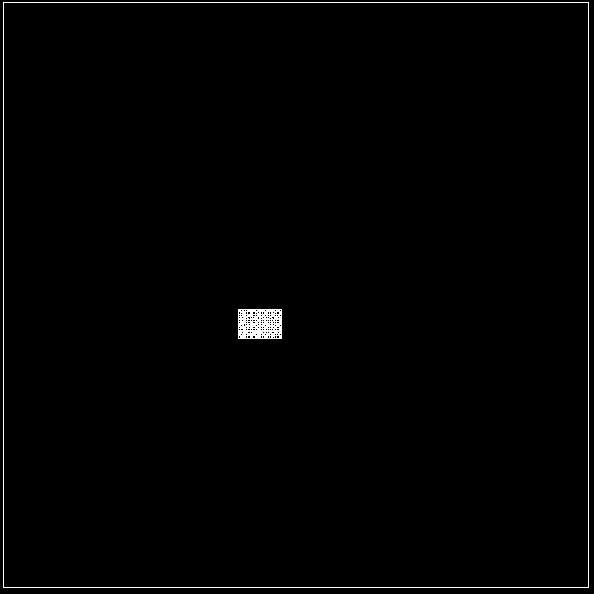
\includegraphics[scale=0.25]{Kap2/ecal-inner-section-cropped-geometry-1.png}\label{fig:cropped-geometry-1}}\hspace{2em}
  \subfloat[Detector simulation zoomed]{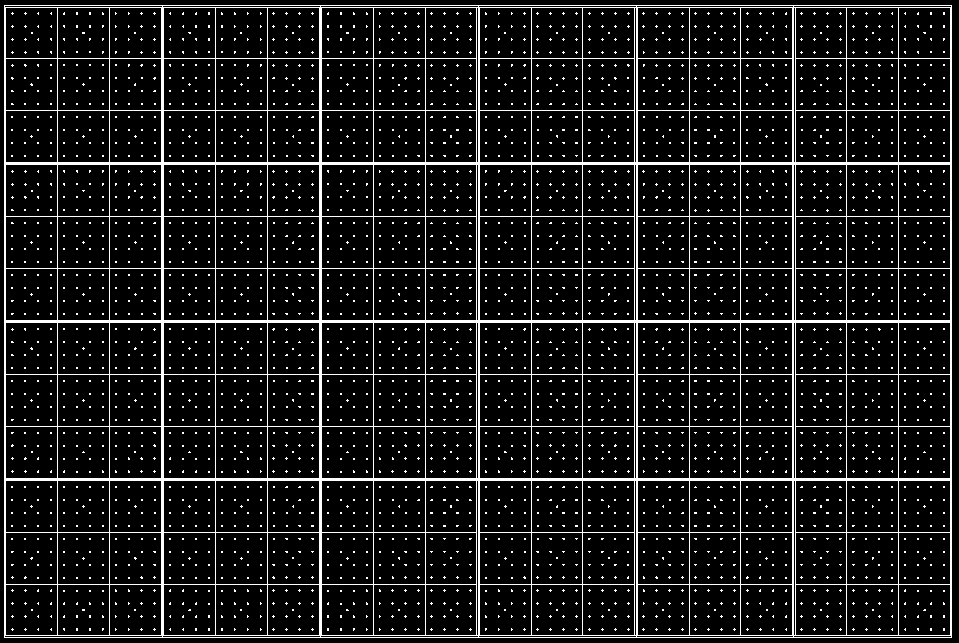
\includegraphics[scale=0.25]{Kap2/ecal-inner-section-cropped-geometry-2.png}\label{fig:cropped-geometry-2}}

  \caption{Front view of the detector. In \ref{fig:cropped-geometry-1}, the
  white square correspond to the caolrimeter and the black is the simulated
  void world box.}\label{fig:cropped-geometry}

\end{figure}

In each module, the scintillator tiles are divided in nine pieces of the same
size, making a mesh of \(3\times3\), while the lead tiles are whole pieces. All
of them have a set of holes as shown in the \cref{fig:module-geometry}, where
WSL wires are placed. All the modules have a recovery of stainless steel of
\(\SI{1}{\cm}\) thick.

\begin{figure}[htb]
  \centering

  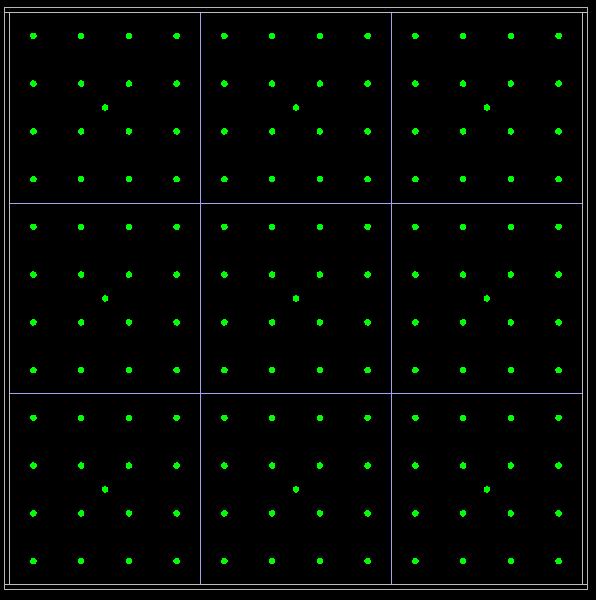
\includegraphics[scale=0.5]{Kap2/Mesh.png}
  \caption{Front view of a single detector module.}\label{fig:module-geometry}

\end{figure}

As explained above, electrons, photons and neutral pions of
\(\SI{20}{\giga\electronvolt}\) were used as primary particles. The primary
particle was placed \(\SI{13}{\metre}\) from the calorimeter.

For each event, the simulation collects information on the number of photons
and electrons created in each of the scintillator and lead layers. For this, it
stores the coordinates of the plate in the detector. It also saves the step
length and the energy deposited on each of the plates, for each interaction
between a particle and that layer. All this information is stored in a ROOT
file. A dataset with \(10000\) events per primary particle was created.

\section{Machine Learning Implementation}

\subsection{Kolmogorov Test}

It should be noted that not all calorimeter plates have photons or electrons
created in them, or in general no particles interact in these layers and
therefore do not contain any information, also the distribution of photons and
electrons created, the step length and the energy deposited in each of the
plates is the same for each of the primary particles, so it is not significant
when applying the classification algorithm. Because of this, a filter was
performed to obtain the significant cells, which will be taken into account in
the machine learning implementation.

A Kolmogorov test were applied for the distribution of all the measured
variables in each of the plates in the detector. This test is used to determine
whether the two histograms are compatible with the same
distribution\cite{root,kolmogorov}. Applying this test, the cells with similar
distributions will be excluded from the machine learning input, since they do
not add significant information to the classifier to separate the primary
particles. The cells that got less than \(0.5\) in the Kolmogorov test were
taken into account in the machine learning implementation.

\subsection{Machine Learning Algorithm}

The machine learning algorithm was built using the Scikit Learn library for
python. The following five multidimensional classifiers were used:
MultinomialNB, BernoulliNB, Perceptron, SGDClassifier,
PassiveAggressiveClassifier. MultinomialNB and BernoulliNB classifiers are both
Naive Bayes methods, that uses the Bayes’ theorem with the assumption that
every pair of features is independent of each other given the class
variable\cite{zhang2004optimality,NBsklearn,scikit-learn}. The difference
between the two algorithms is that the Bernoulli Naive Bayes method explicity
penalizes the non-occurrence of a feature that is an indicator of a given
class\cite{NBsklearn}.

The Perceptron and the PassiveAggressiveClassifier are Linear methods, it means
that they consider that the target class can be expressed as a lineal
combination of the features\cite{LMsklearn,scikit-learn}. Both methods do not
require a learning rate, but the the PassiveAggressiveClassifier includes a
regularizatión parameter while Perceptron does not. Finally, SGDClassifier use
the Stochastic Gradient Descent routing for fitting a linear classifier. It
allow the use of different loss functions and penalties for
classification\cite{SGDsklearn,scikit-learn}.

These classifiers were chosen due to the size of the input set, even after
getting information just from significant cells, the arrays were too large,
then it is computationally easier to partially fit the model with each new data
vector. The data from the simulation was divided in two groups, \(5000\) events
each one, that worked as train and test set respectively.

\chapter{Results}

At first, from the simulated dataset, the distribution of photons and electrons
creation in each of the plates of the calorimeters was plotted, as well as the
step length and energy deposit for each interaction. The number of electrons or
photons created in the plates for each material are divided in two plots.
First, a two-dimensional histogram illustrates the front view of the
calorimeter, giving the distribution of the particle generation in the X-Y
plane. The second plot correspond a one-dimensional histogram that shows the
distribution in the Z axis.

\begin{figure}[htb!]
  \centering

  \subfloat[\(e^-\) as primary particle, X-Y plane of the calorimeter.]{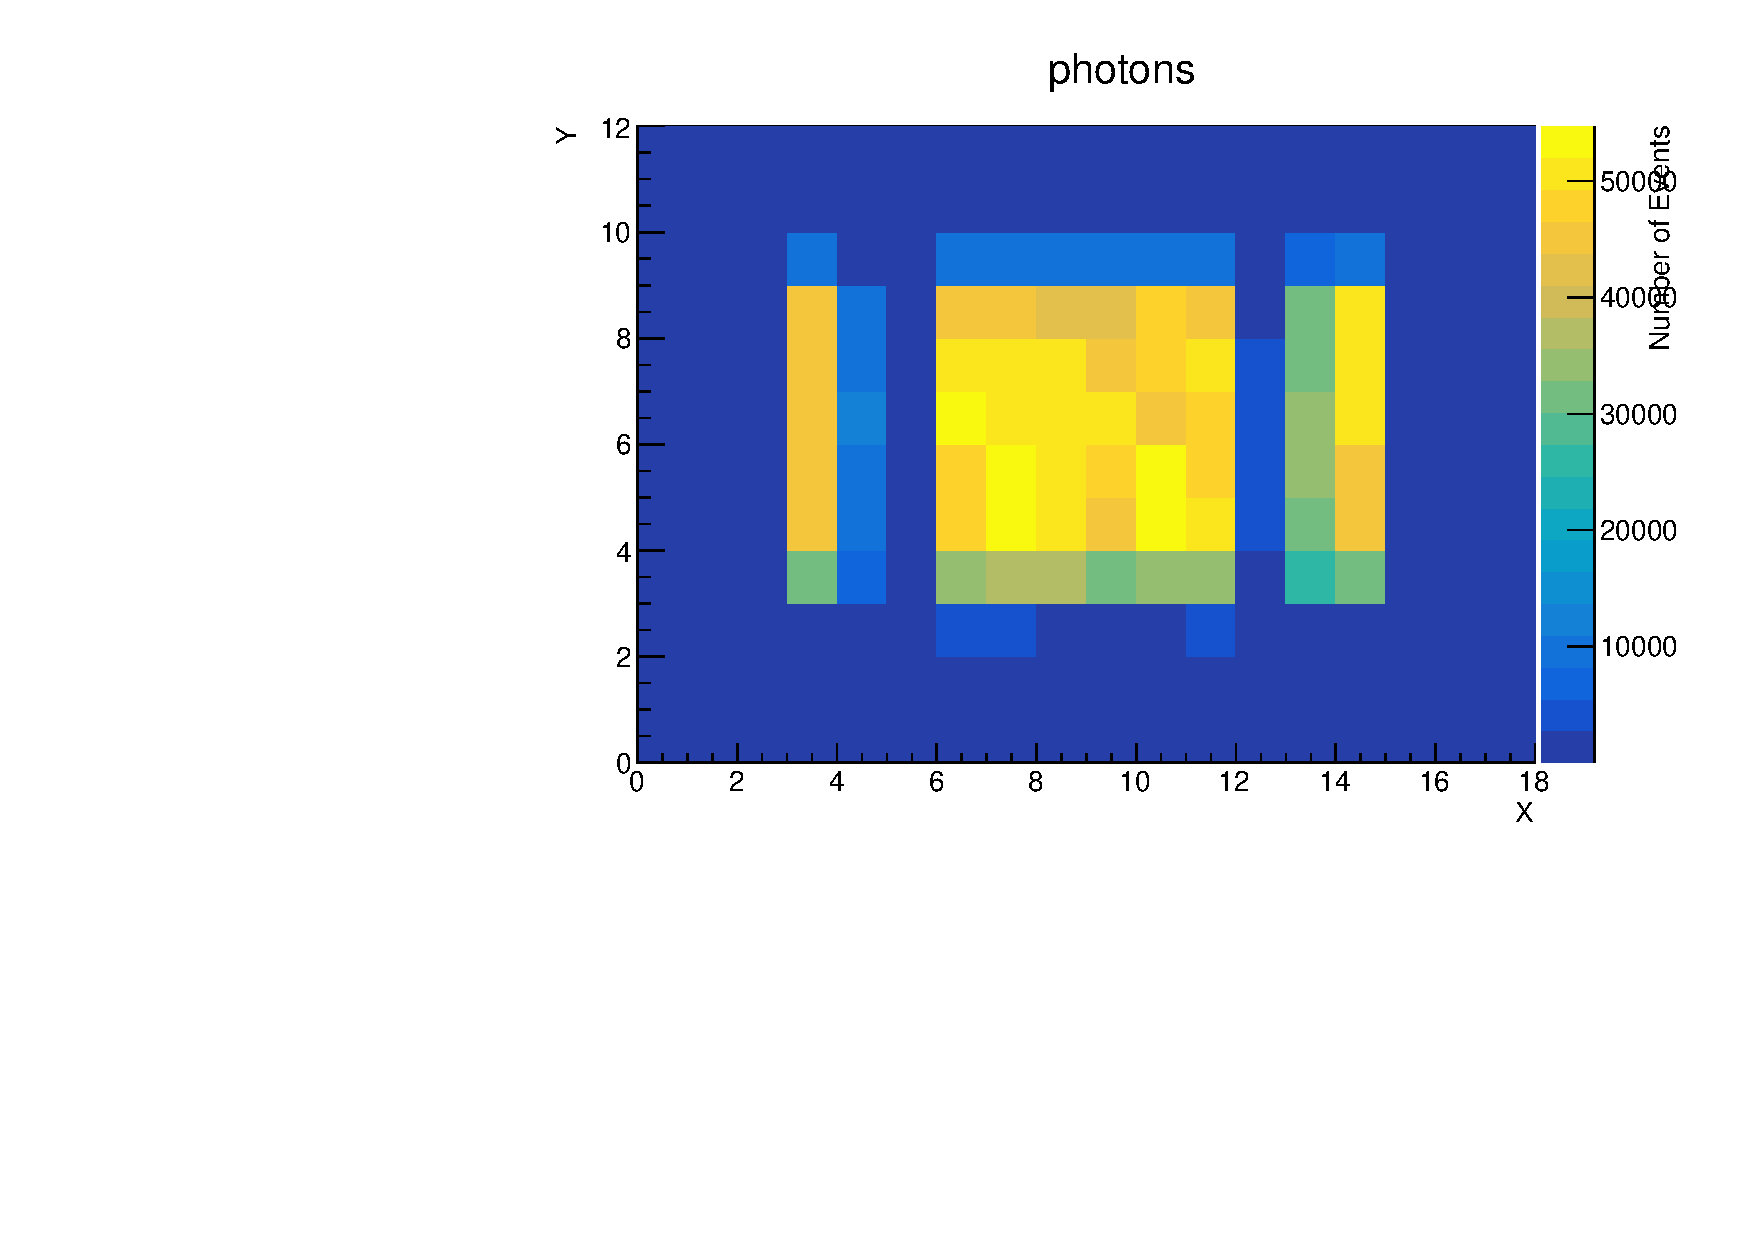
\includegraphics[scale=0.35]{Kap3/electron_scintillator_photons_plots_calo_counter.pdf}\label{fig:photons-creation-scintillator-1}}\hspace{1em}
  \subfloat[\(e^-\) as primary particle, Z axis of the calorimeter.]{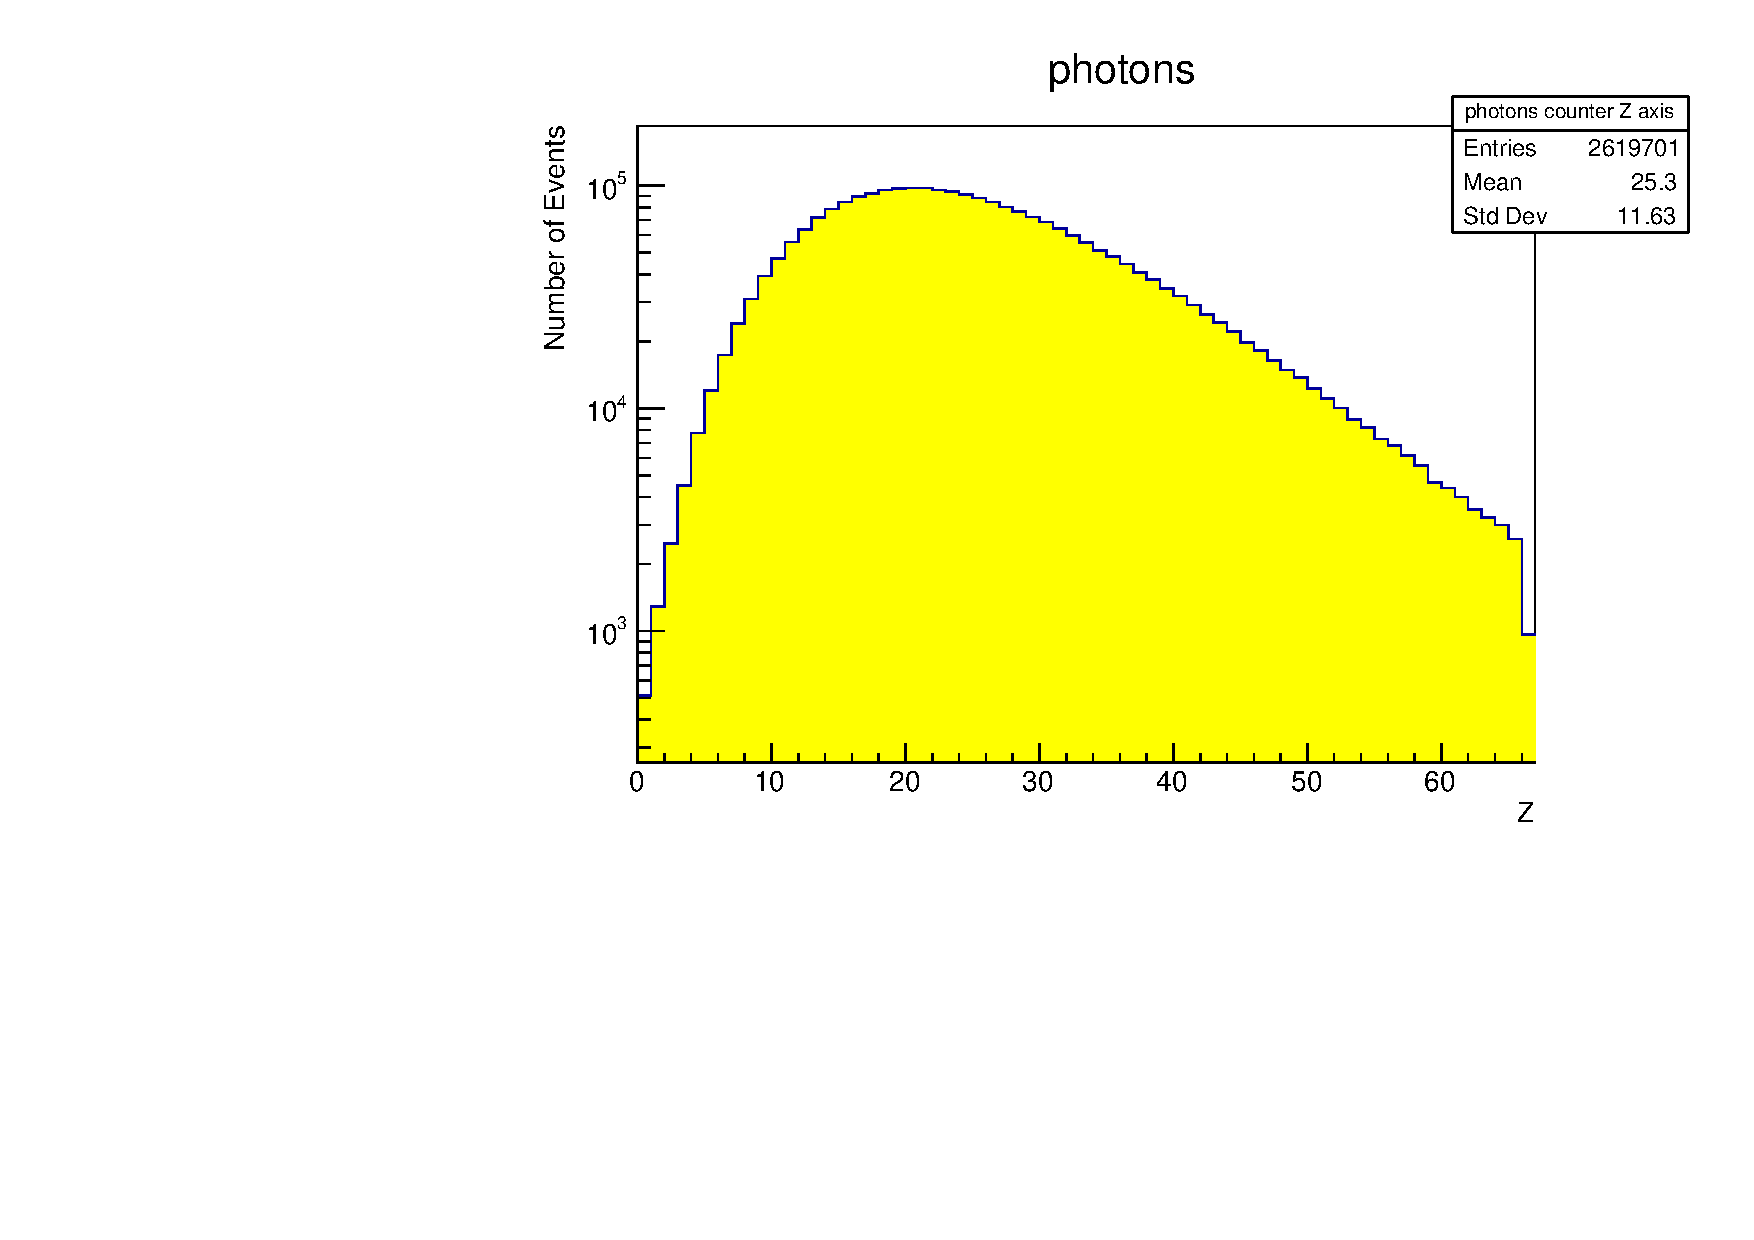
\includegraphics[scale=0.35]{Kap3/electron_scintillator_photons_plots_calo_counter_Z.pdf}\label{fig:photons-creation-scintillator-2}}

  \subfloat[\(\gamma\) as primary particle, X-Y plane of the calorimeter.]{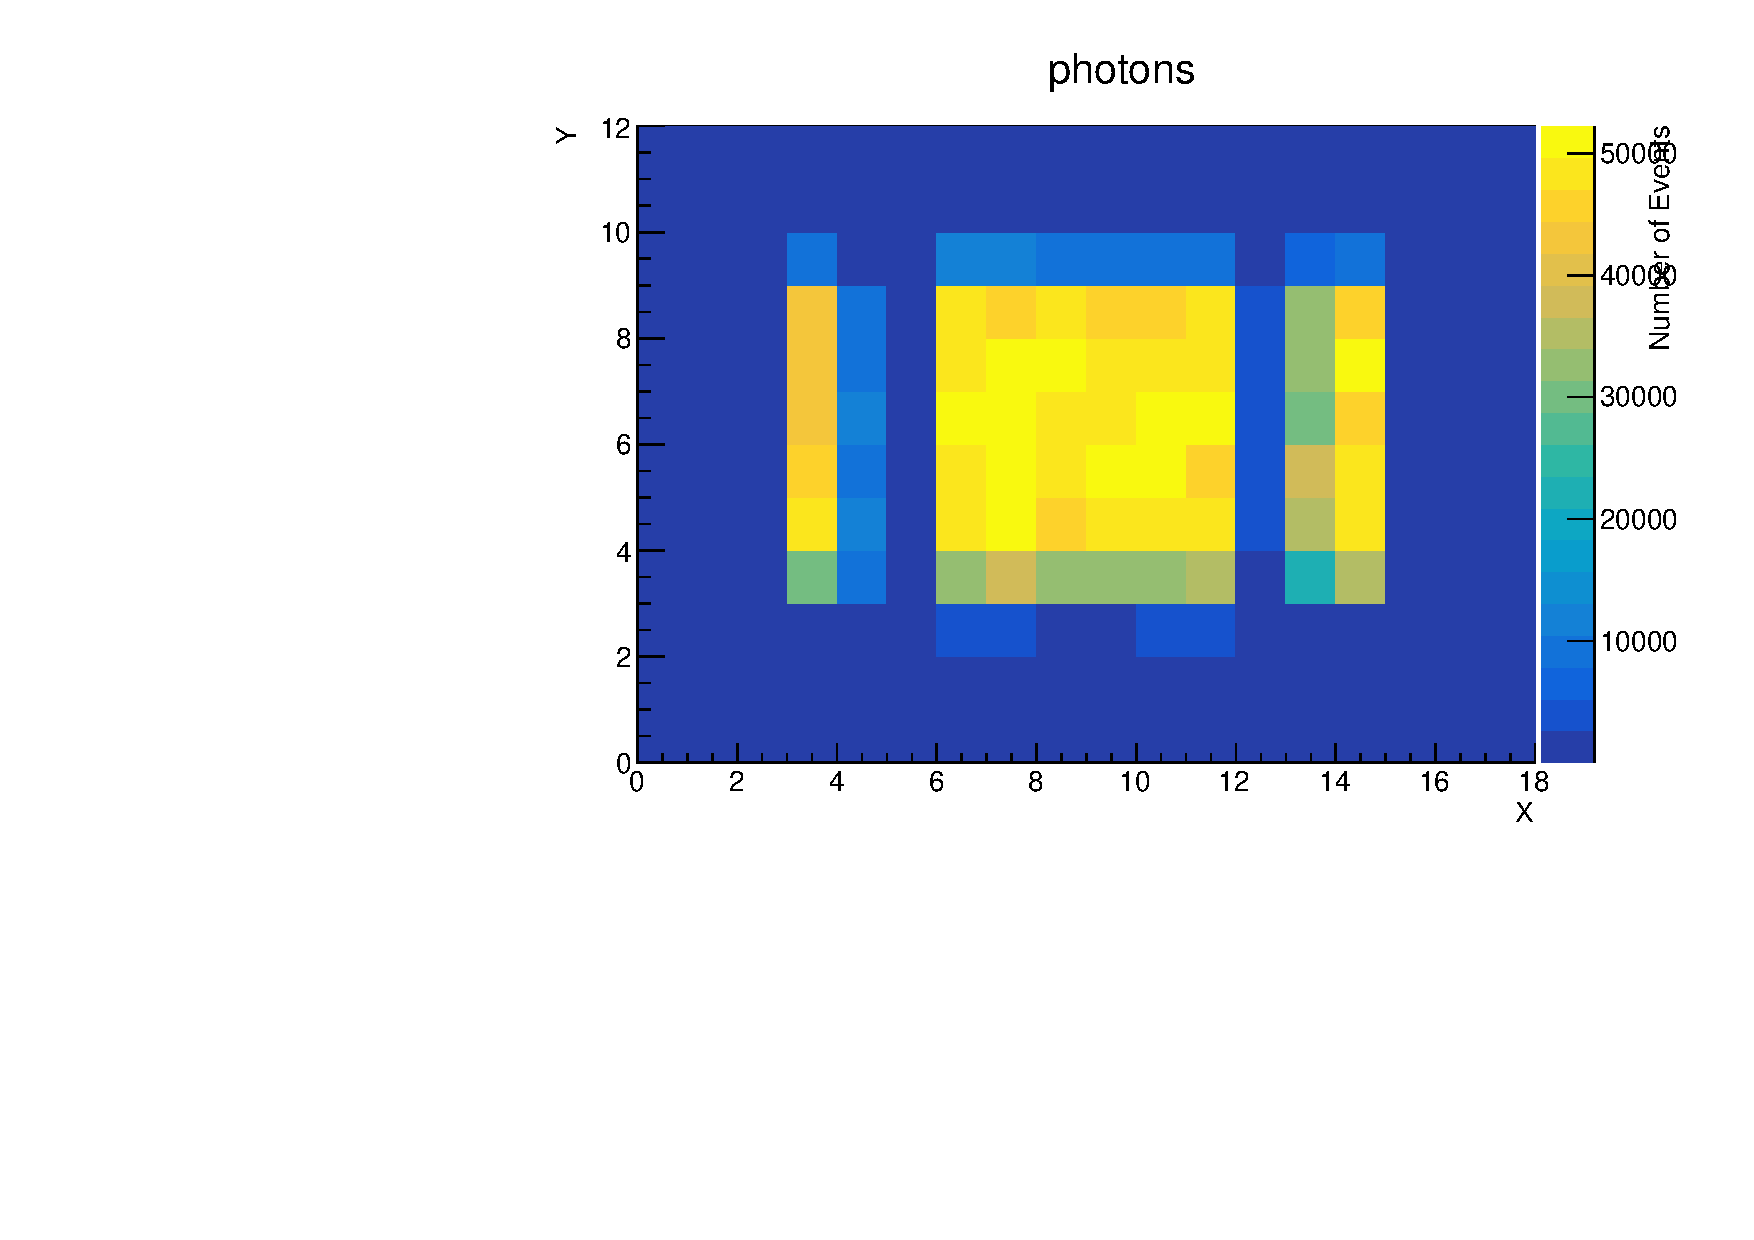
\includegraphics[scale=0.35]{Kap3/gamma_scintillator_photons_plots_calo_counter.pdf}\label{fig:photons-creation-scintillator-3}}\hspace{1em}
  \subfloat[\(\gamma\) as primary particle, Z axis of the calorimeter.]{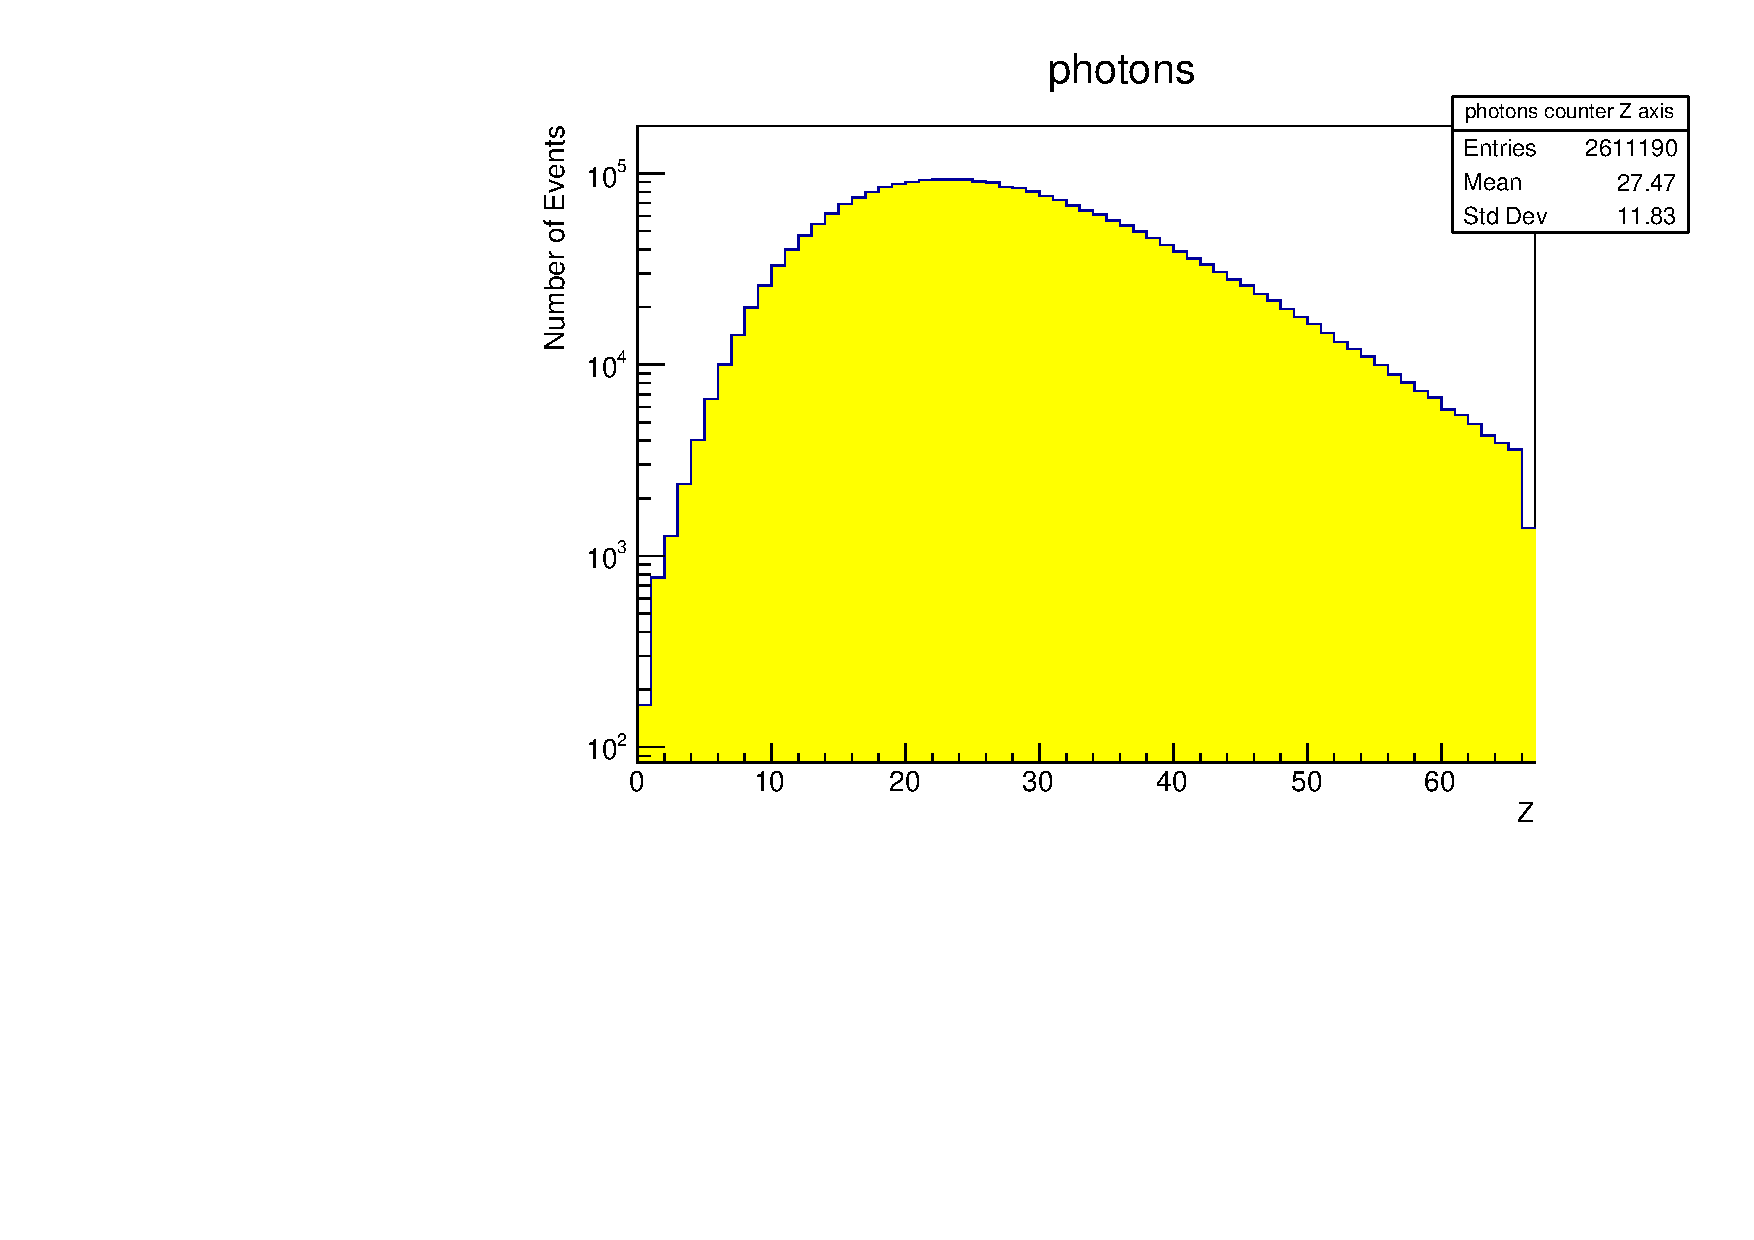
\includegraphics[scale=0.35]{Kap3/gamma_scintillator_photons_plots_calo_counter_Z.pdf}\label{fig:photons-creation-scintillator-4}}

  \subfloat[\(\pi^0\) as primary particle, X-Y plane of the calorimeter.]{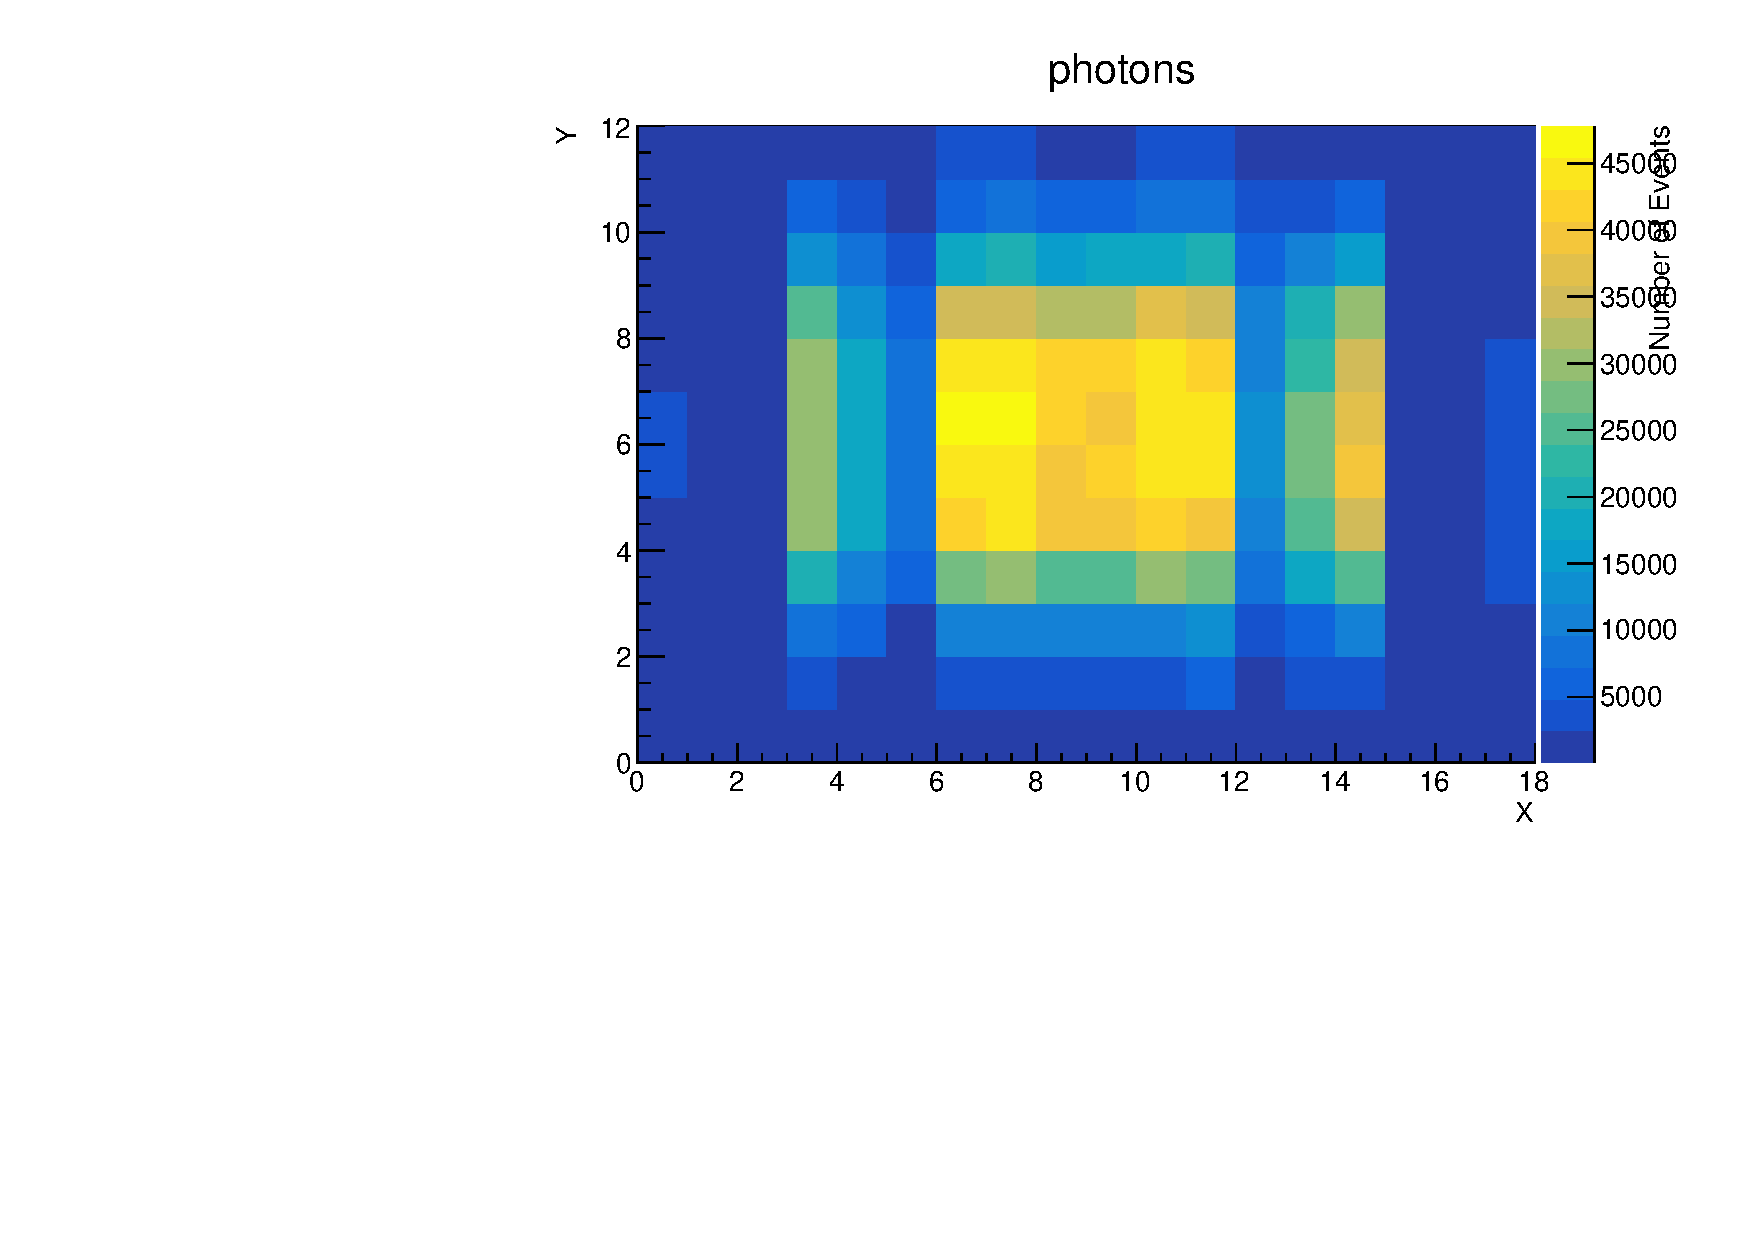
\includegraphics[scale=0.35]{Kap3/pi0_scintillator_photons_plots_calo_counter.pdf}\label{fig:photons-creation-scintillator-5}}\hspace{1em}
  \subfloat[\(\pi^0\) as primary particle, Z axis of the calorimeter.]{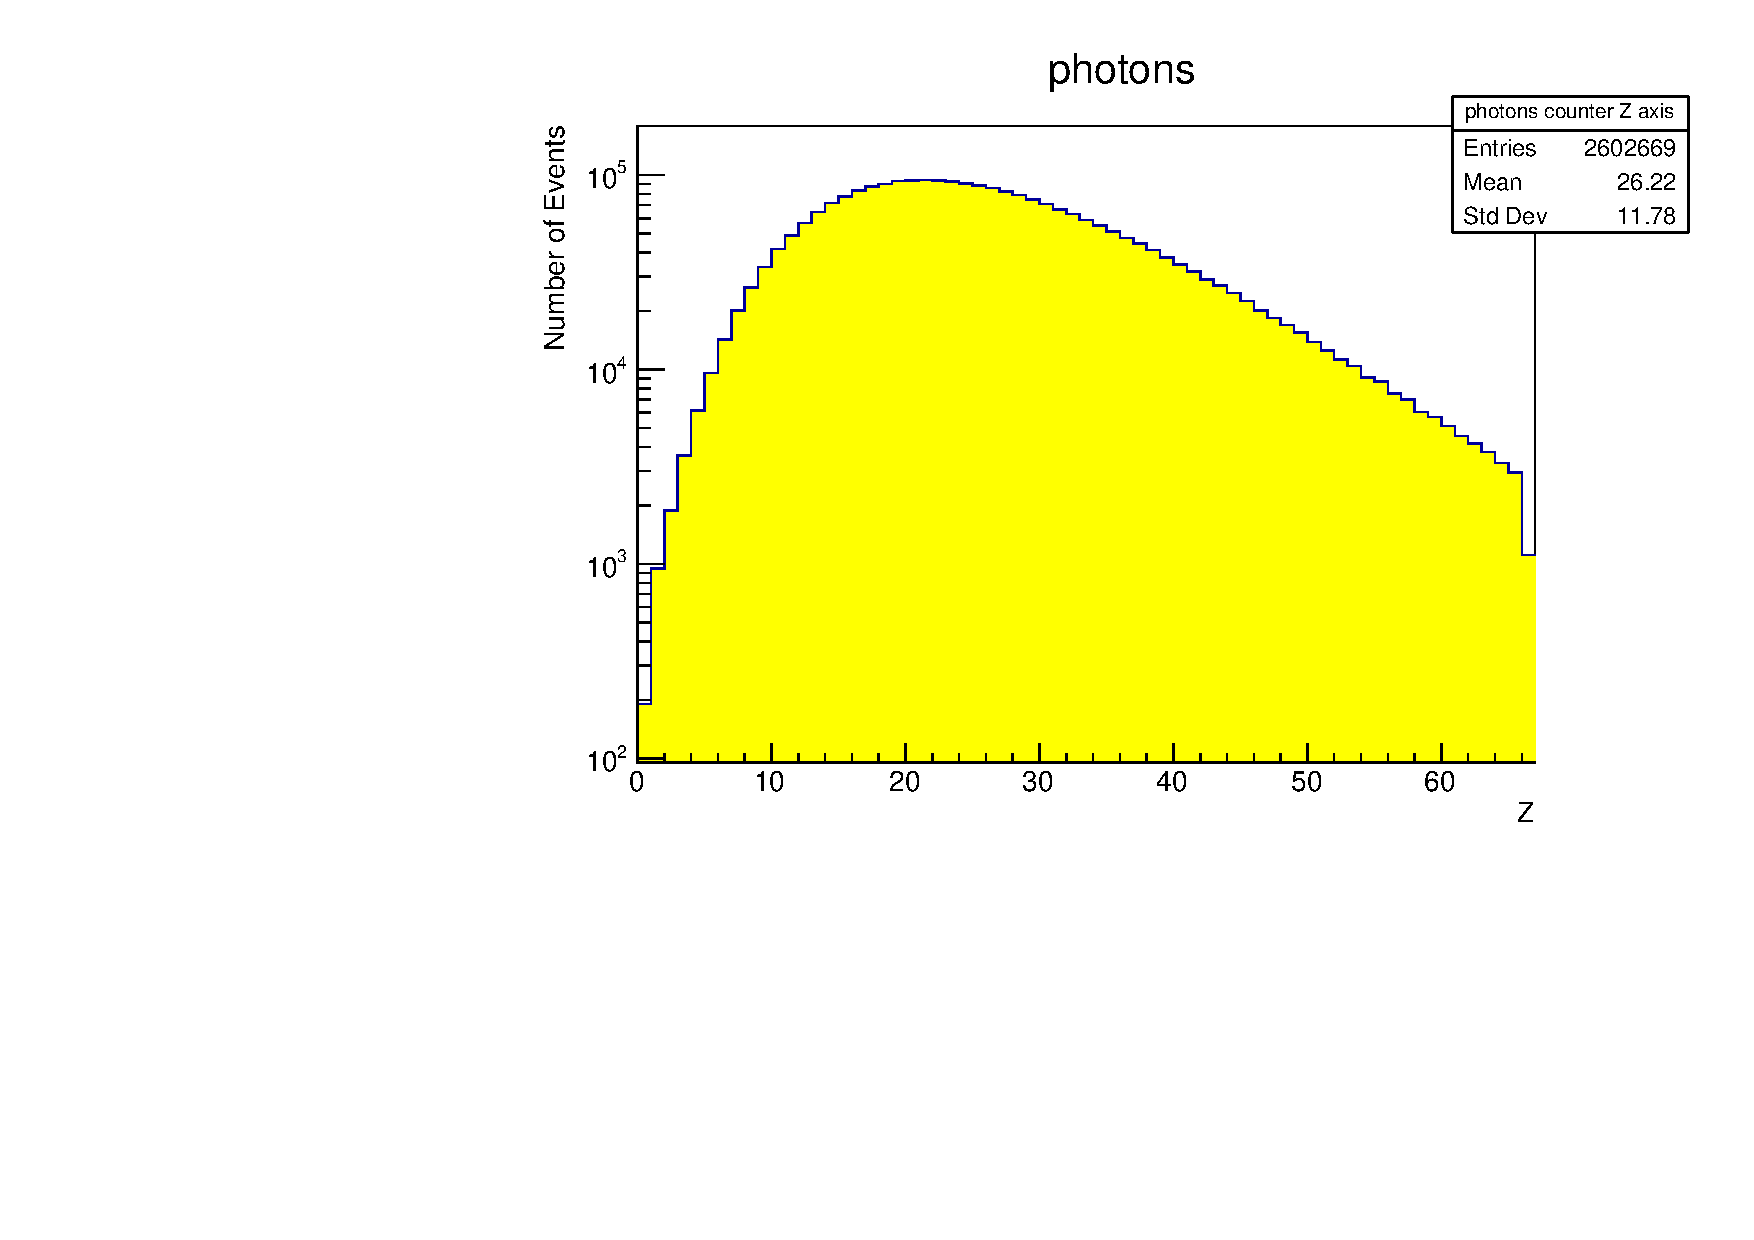
\includegraphics[scale=0.35]{Kap3/pi0_scintillator_photons_plots_calo_counter_Z.pdf}\label{fig:photons-creation-scintillator-6}}

  \caption{Photons creation in the scintillator plates of the calorimeter.}\label{fig:photons-creation-scintillator}

\end{figure}

Let's start with the photon creation in the scintillator plates, as show in the
\cref{fig:photons-creation-scintillator}. In the X-Y plane the mean is at
\((8.777, 5.695)\), \((8.797, 5.702)\) and \(8.755, 5.708\) for electrons,
photons and neutral pions events respectively. In general, the mean value lays
in the center of the mesh. The only noticeable difference is in the standard
deviation that can be seen in the number of events outside the central plates.
The pion signal have a standard deviation of \((3.398, 2.183)\) being larger
than that of electrons of \((3.266, 1.801)\) and photons of \((3.270, 1.805)\),
highlighting that the greatest difference is in the standard deviation of the
vertical axis.

\begin{figure}[htb!]
  \centering

  \subfloat[\(e^-\) as primary particle, X-Y plane of the calorimeter.]{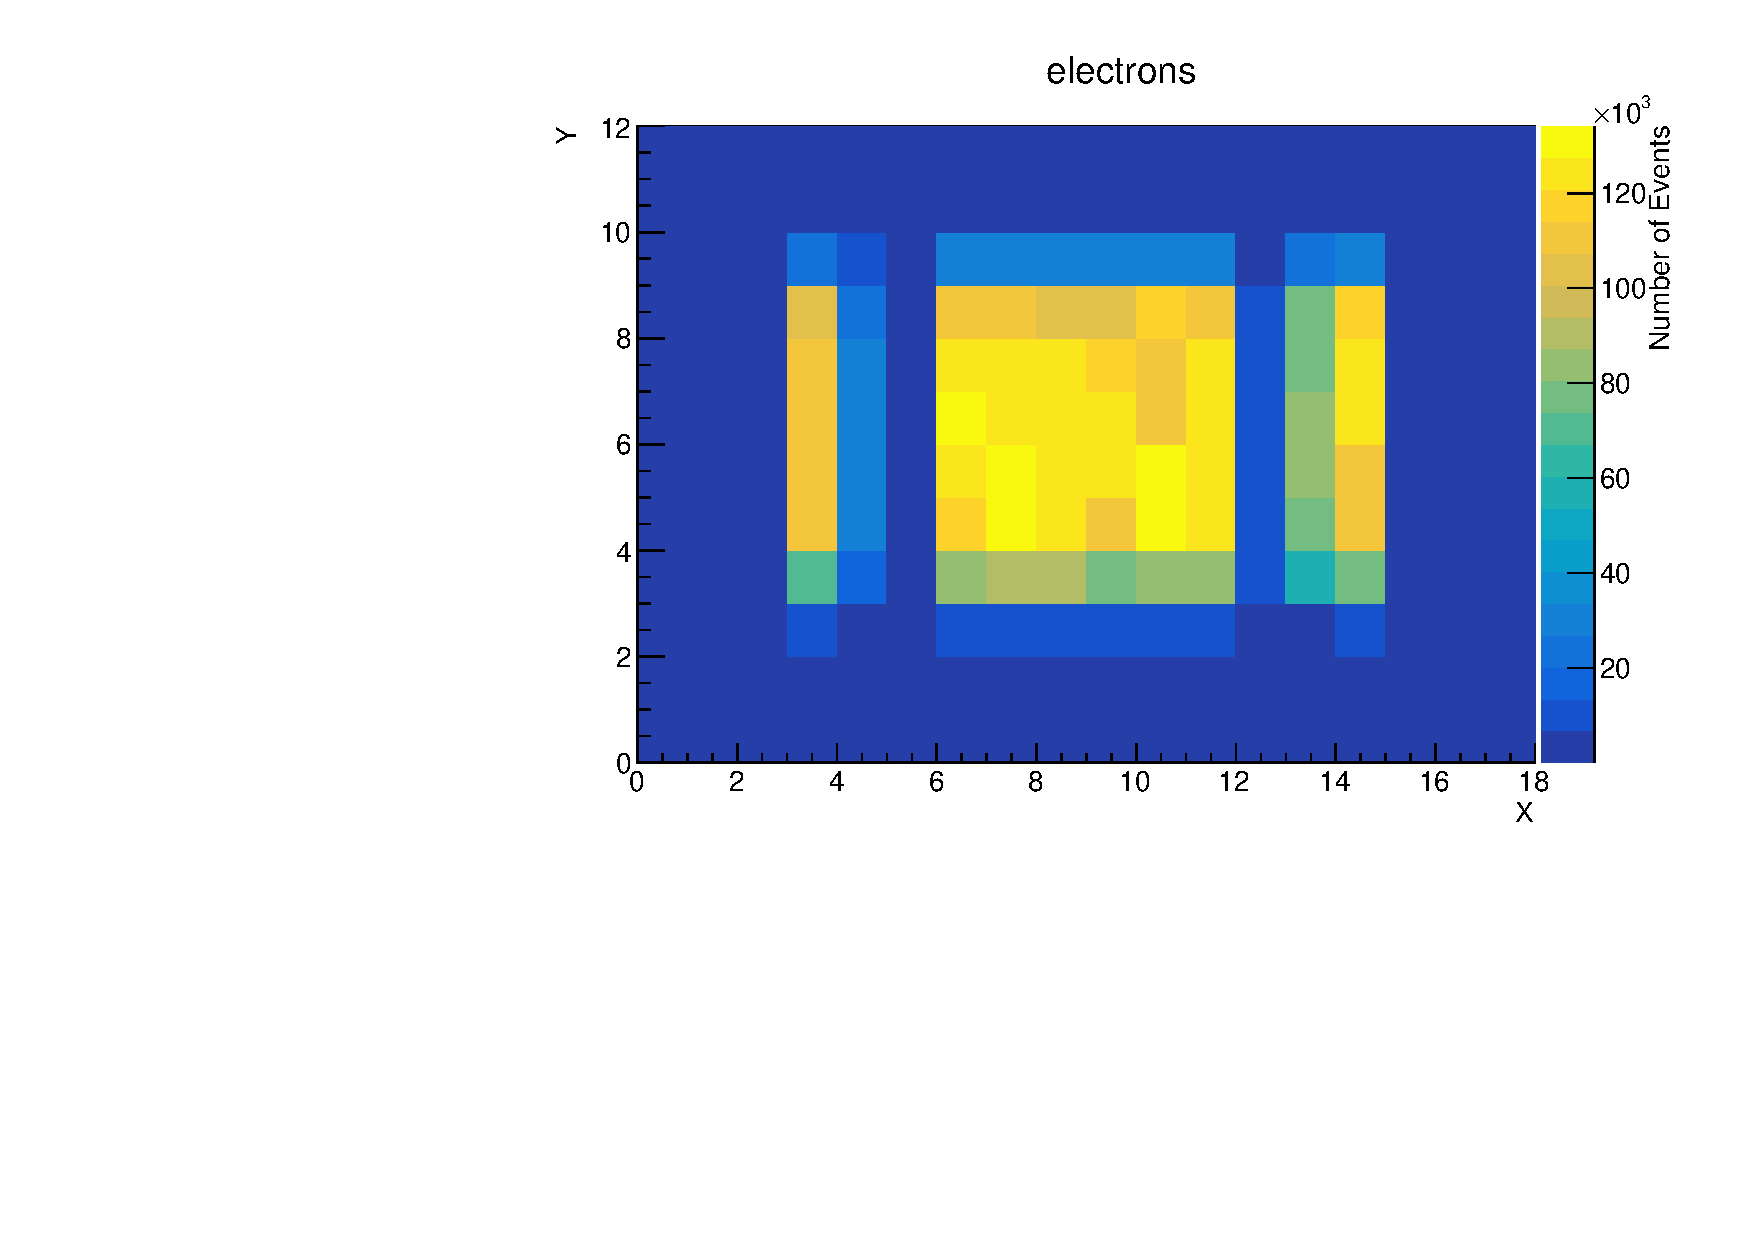
\includegraphics[scale=0.35]{Kap3/electron_scintillator_electrons_plots_calo_counter.pdf}\label{fig:electrons-creation-scintillator-1}}\hspace{1em}
  \subfloat[\(e^-\) as primary particle, Z axis
   of the calorimeter.]{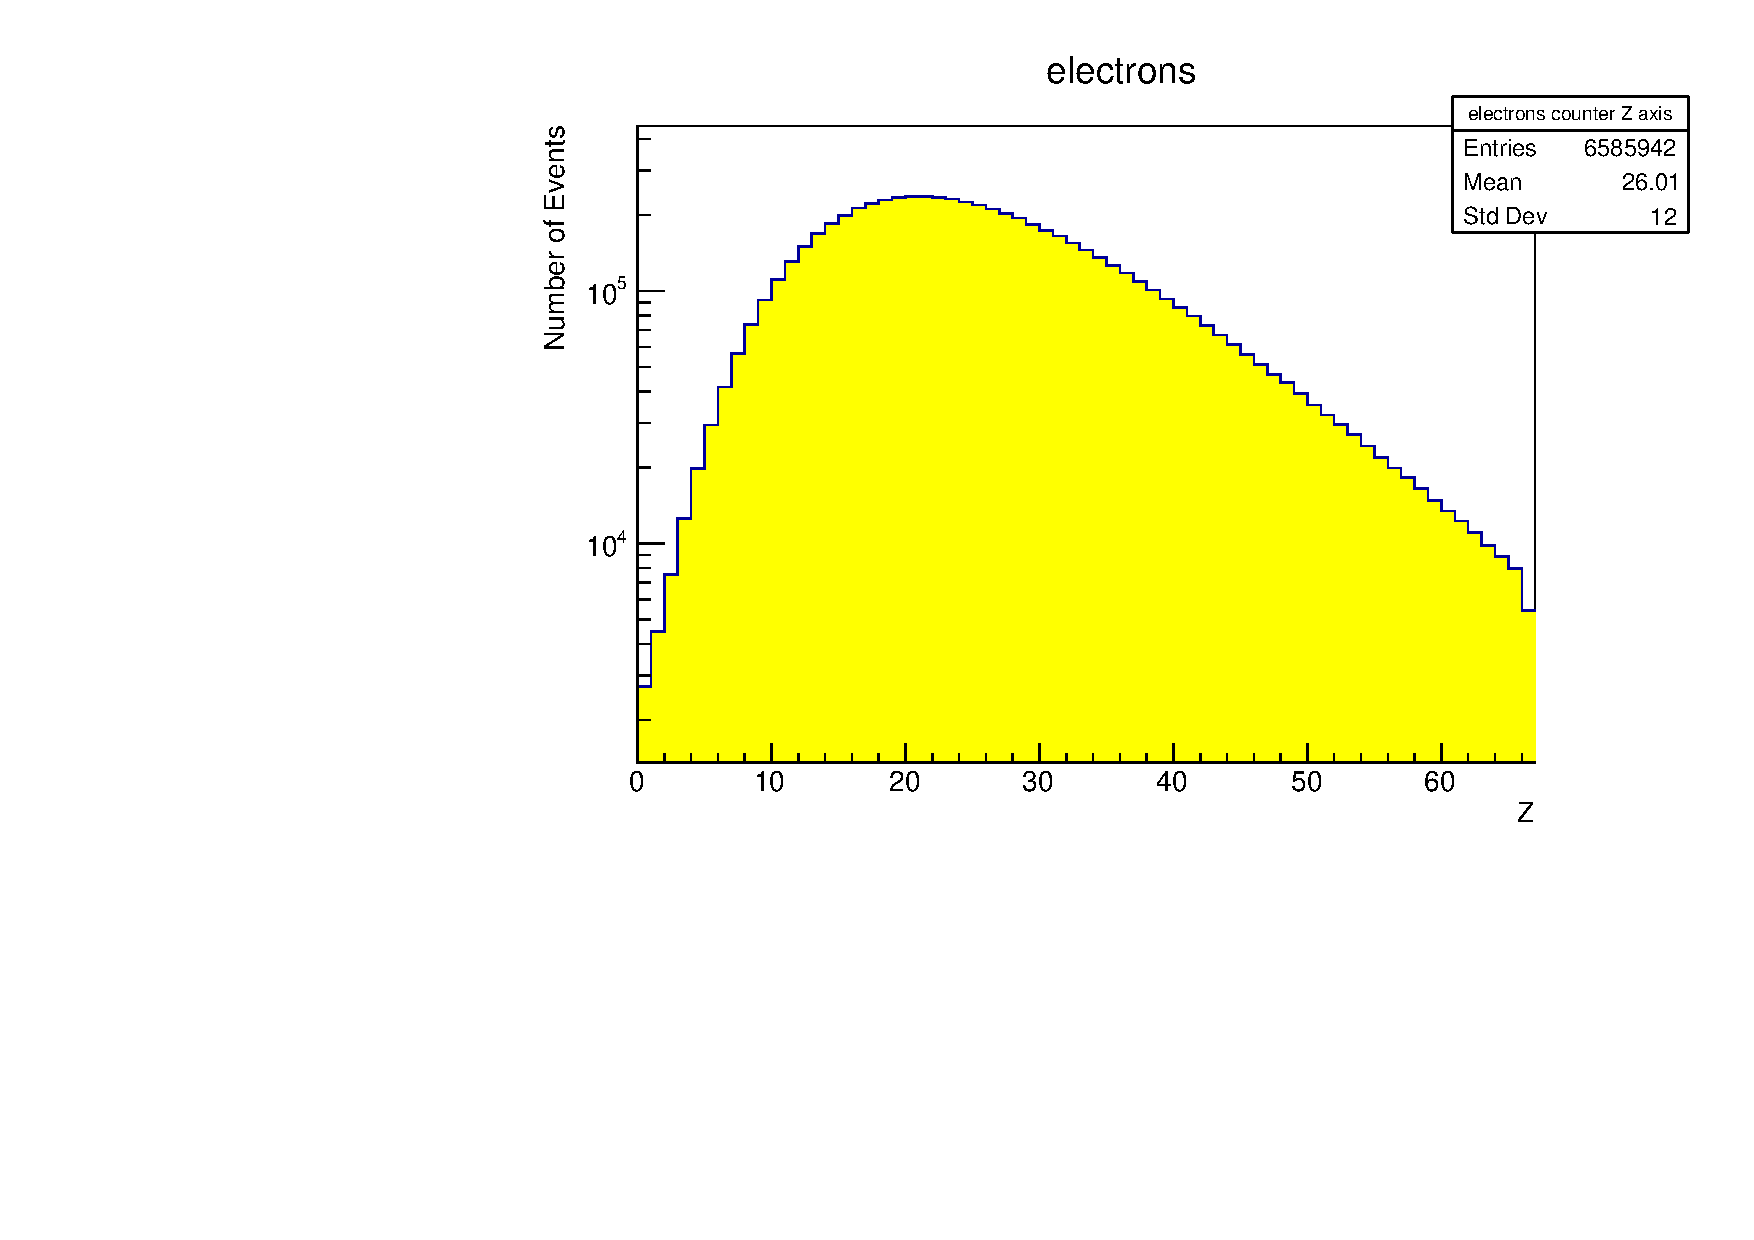
\includegraphics[scale=0.35]{Kap3/electron_scintillator_electrons_plots_calo_counter_Z.pdf}\label{fig:electrons-creation-scintillator-2}}

   \subfloat[\(\gamma\) as primary particle, X-Y plane of the calorimeter.]{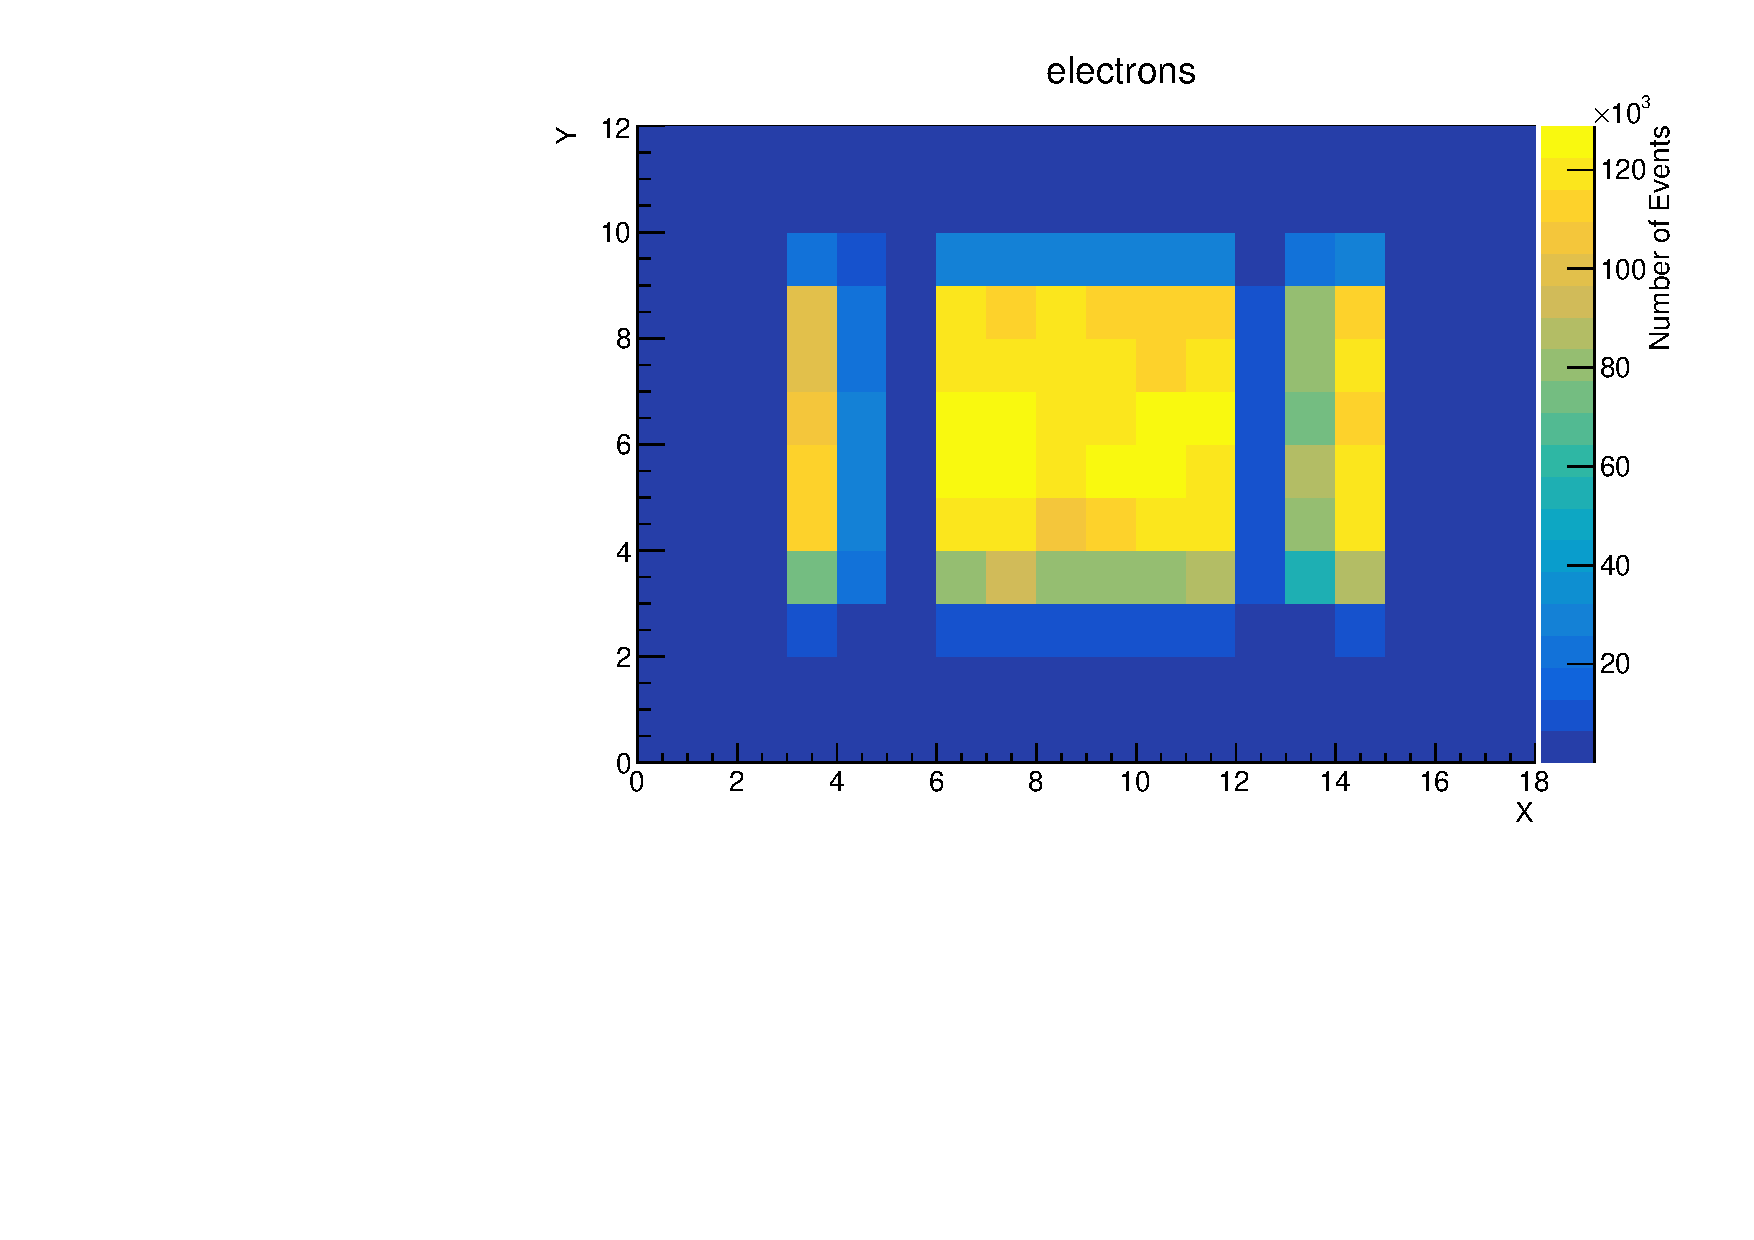
\includegraphics[scale=0.35]{Kap3/gamma_scintillator_electrons_plots_calo_counter.pdf}\label{fig:electrons-creation-scintillator-3}}\hspace{1em}
   \subfloat[\(\gamma\) as primary particle, Z axis of the calorimeter.]{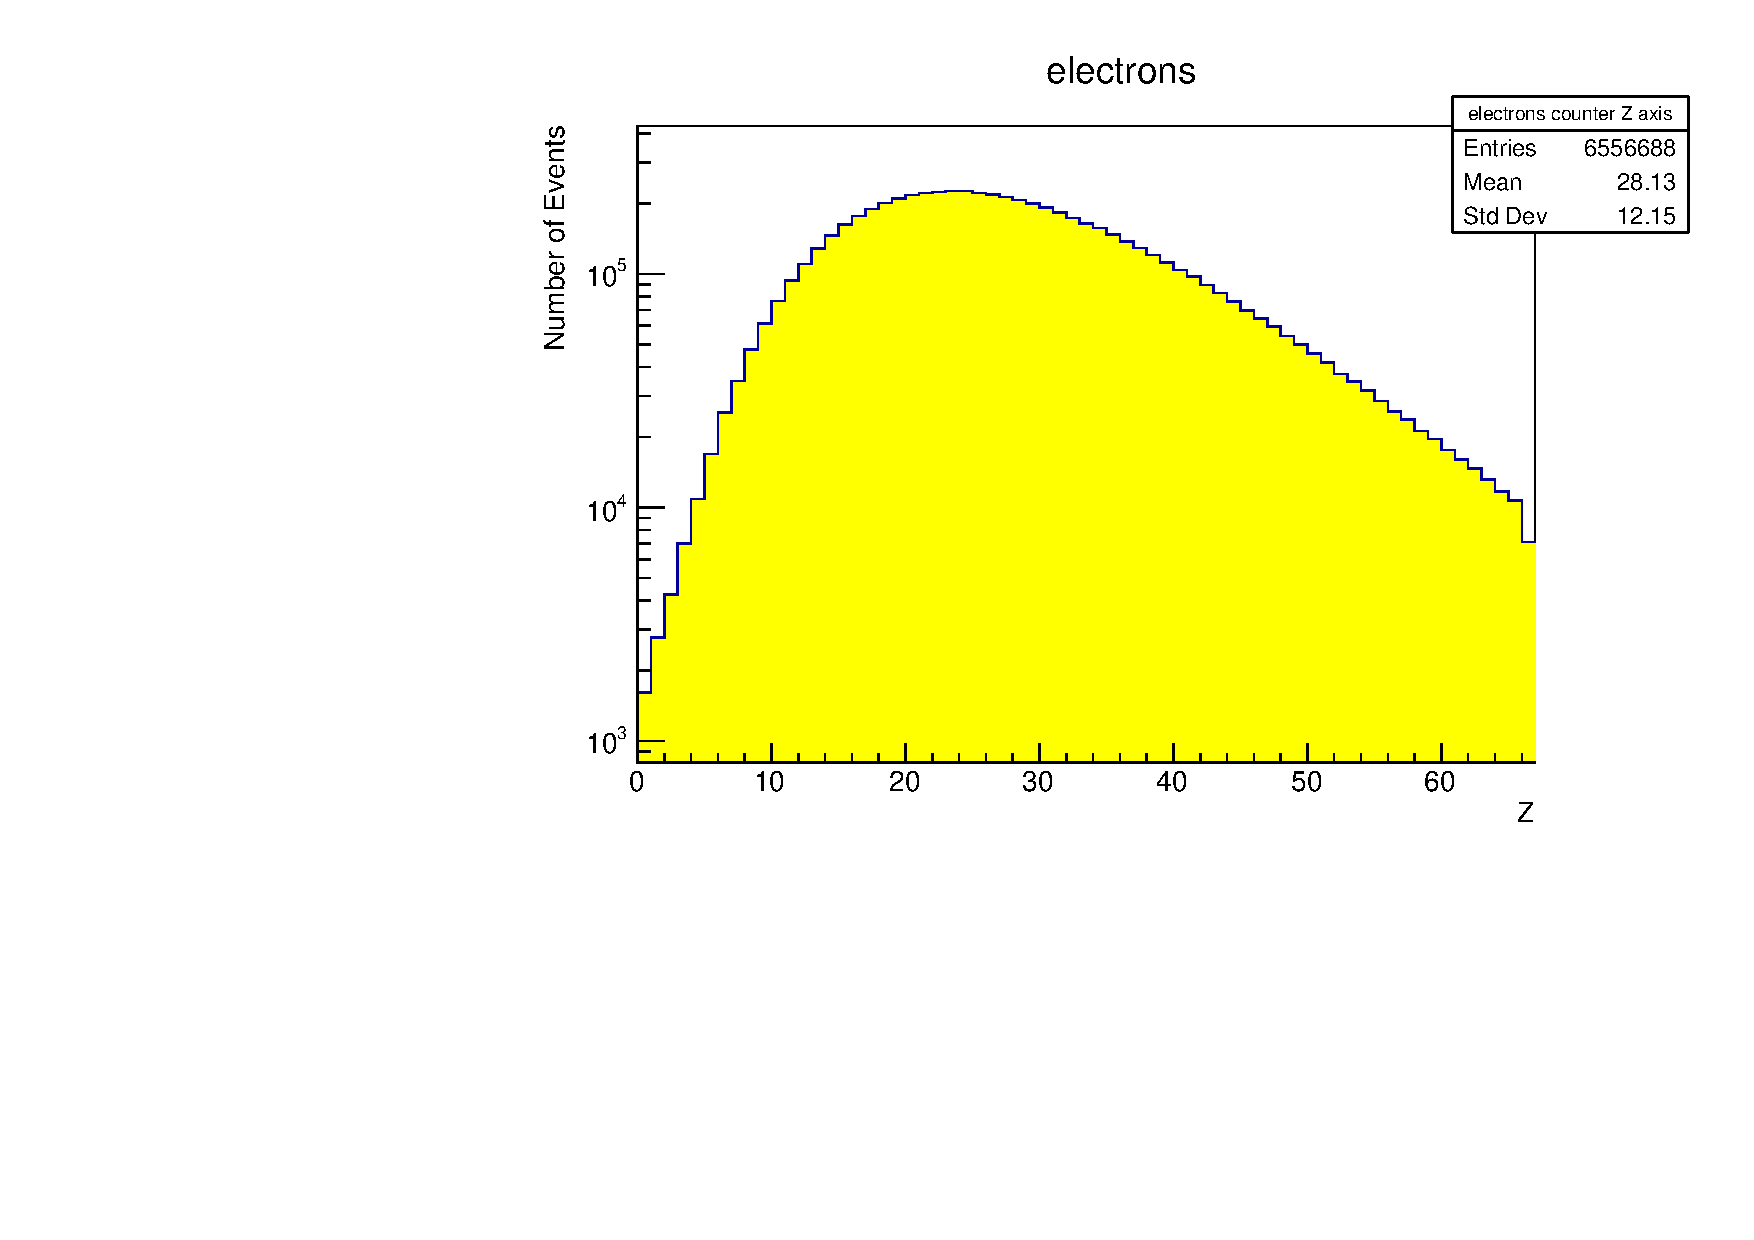
\includegraphics[scale=0.35]{Kap3/gamma_scintillator_electrons_plots_calo_counter_Z.pdf}\label{fig:electrons-creation-scintillator-4}}

   \subfloat[\(\pi^0\) as primary particle, X-Y plane of the calorimeter.]{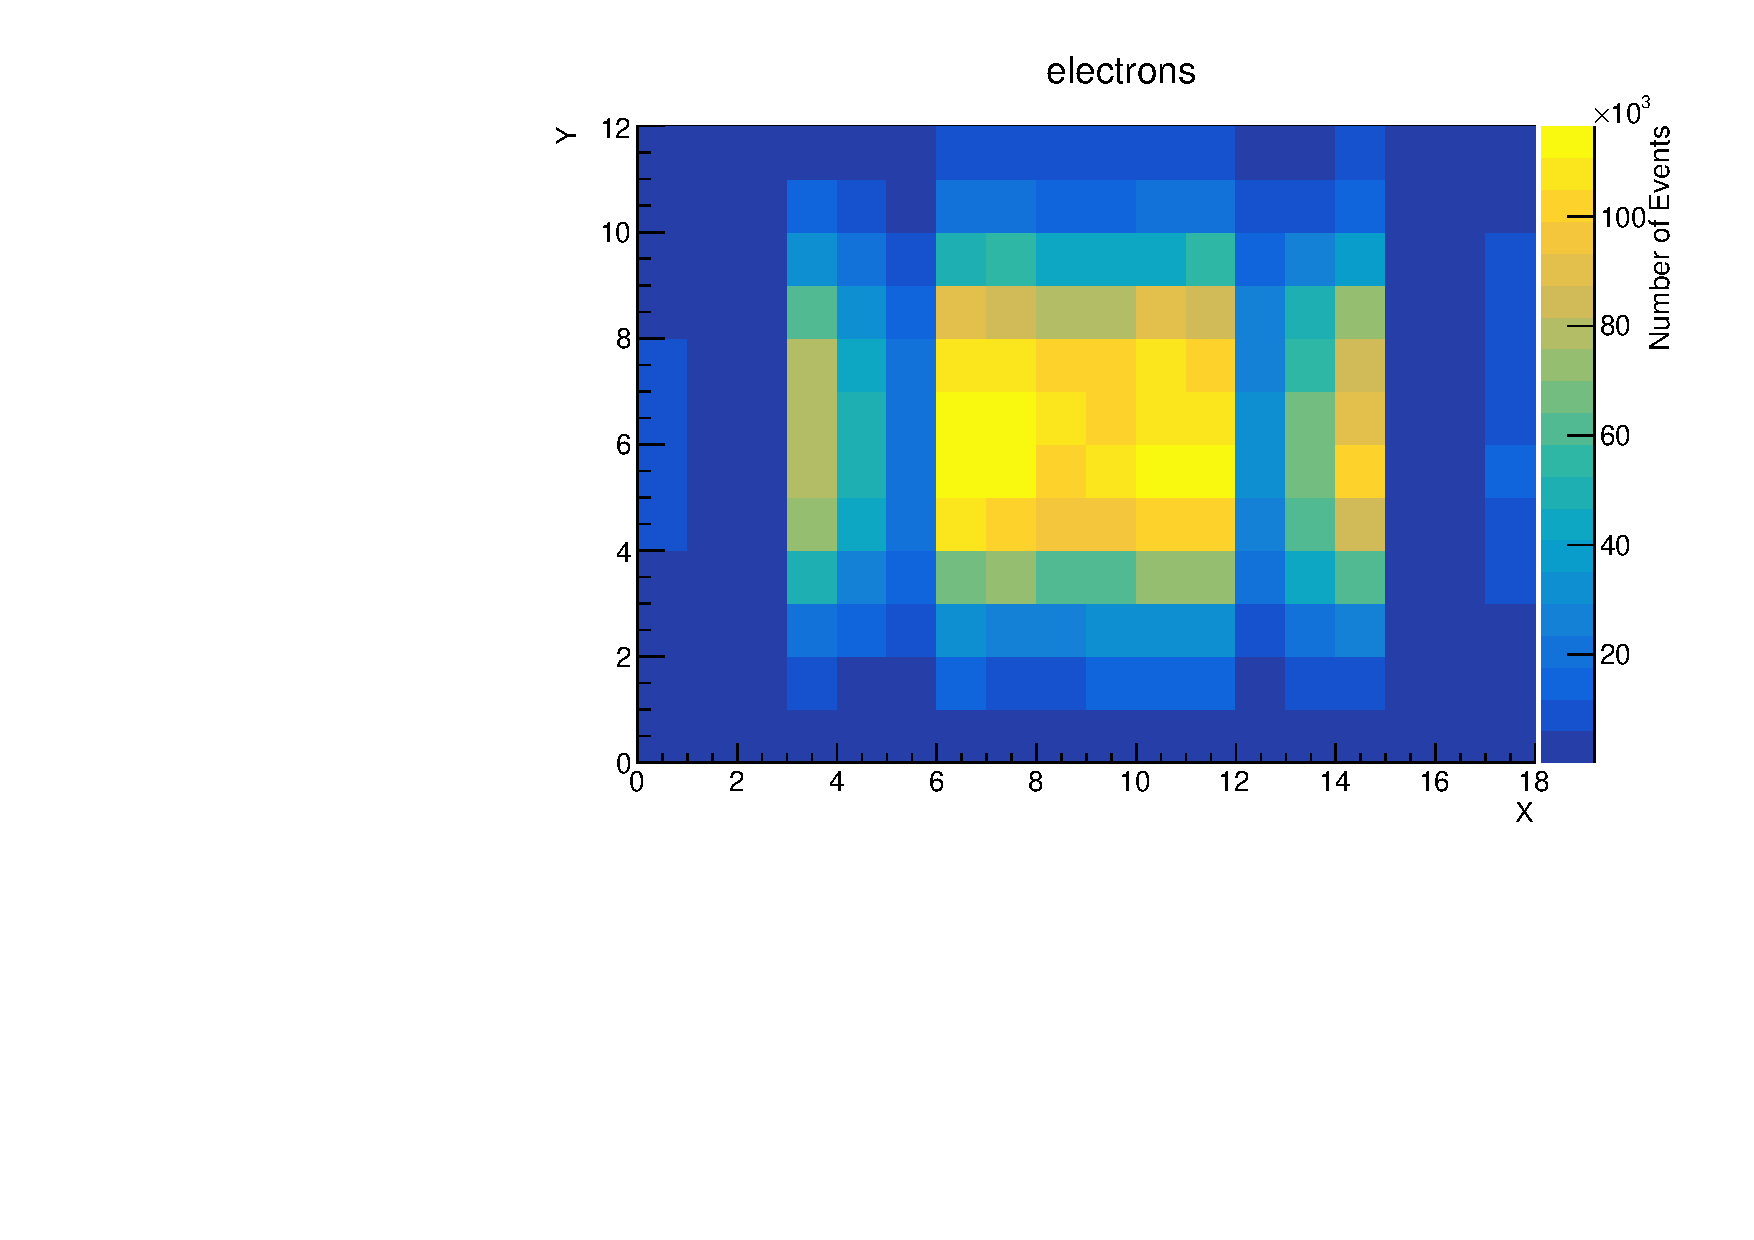
\includegraphics[scale=0.35]{Kap3/pi0_scintillator_electrons_plots_calo_counter.pdf}\label{fig:electrons-creation-scintillator-5}}\hspace{1em}
   \subfloat[\(\pi^0\) as primary particle, Z axis of the calorimeter.]{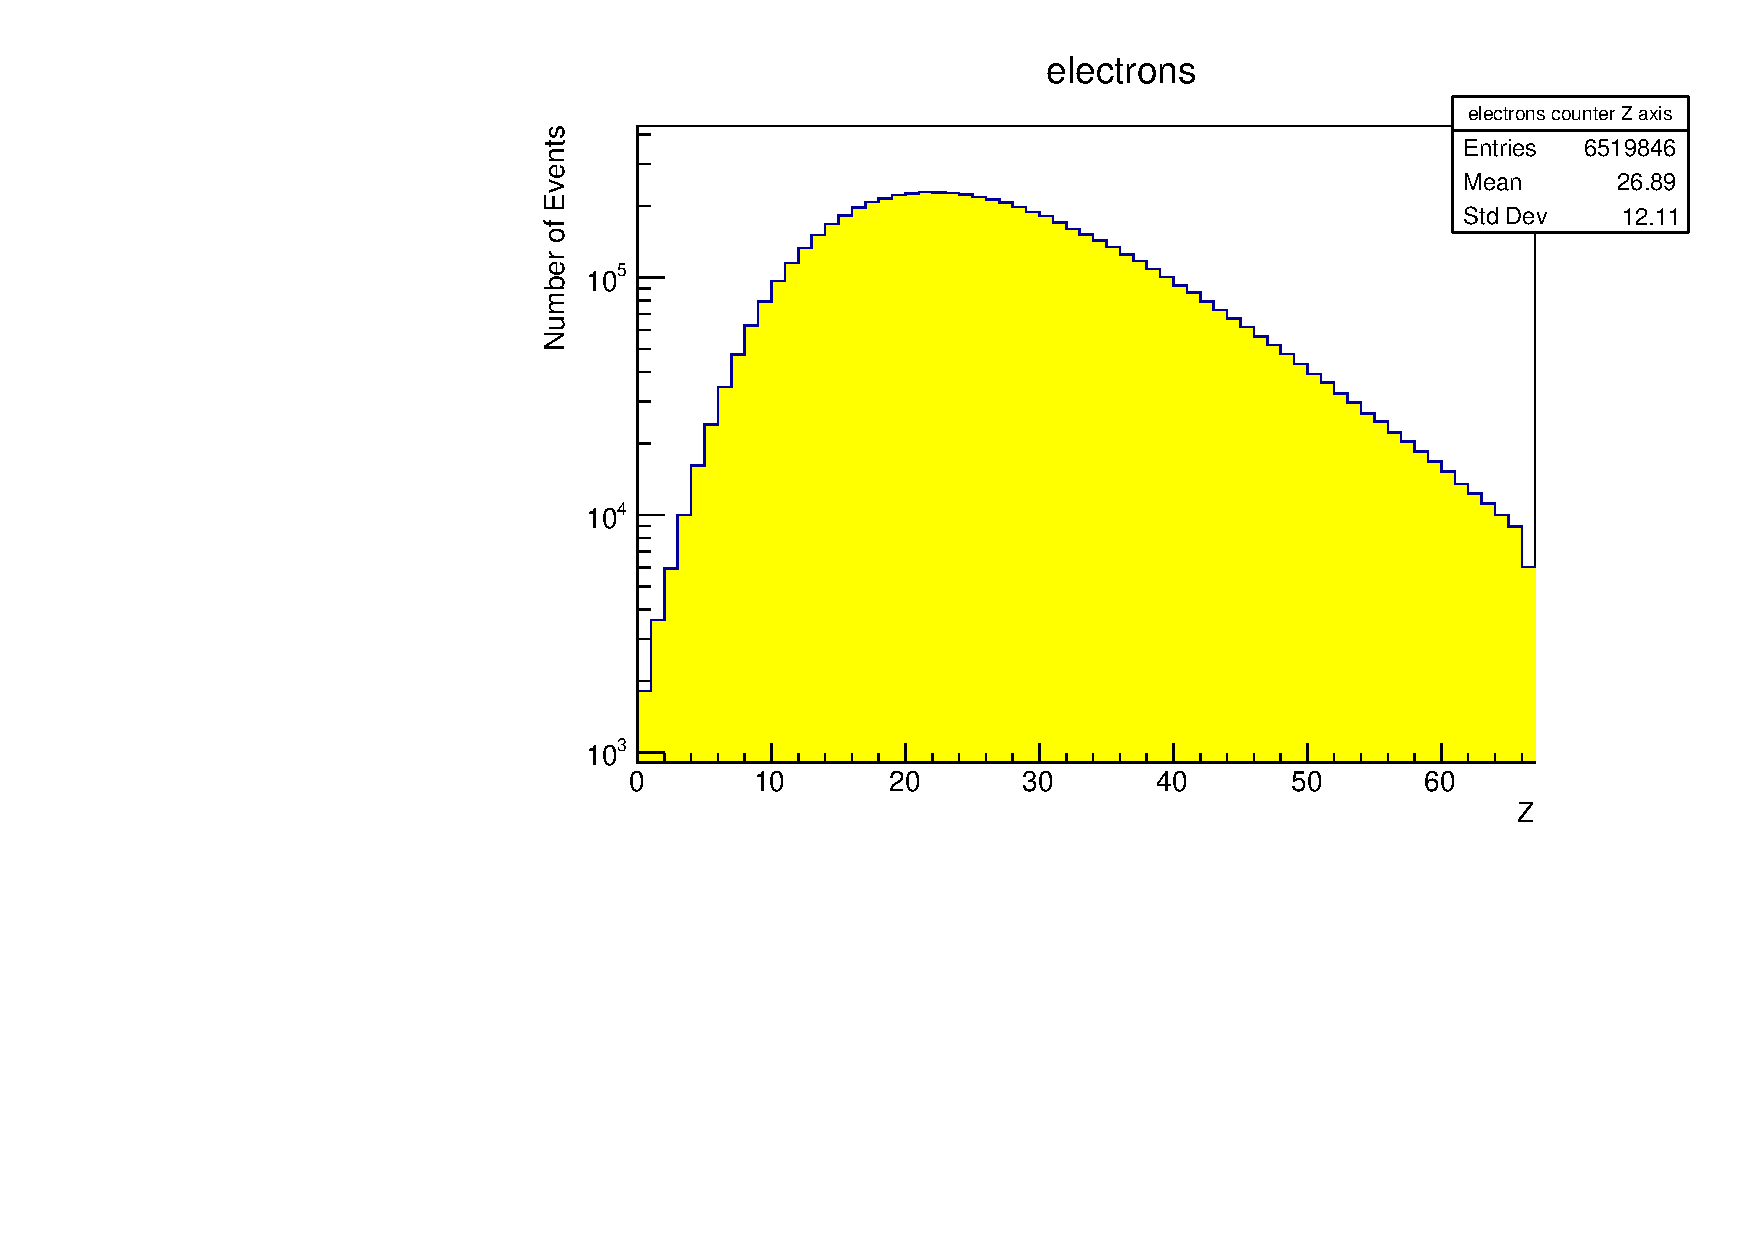
\includegraphics[scale=0.35]{Kap3/pi0_scintillator_electrons_plots_calo_counter_Z.pdf}\label{fig:electrons-creation-scintillator-6}}

  \caption{Electron creation in the scintillator plates of the calorimeter.}\label{fig:electrons-creation-scintillator}

\end{figure}

The same scenario can be seen for the created electrons in the scintillator
plates (see \cref{fig:electrons-creation-scintillator}). Again, the mean is in
the central plates, in this case, \((8.766, 5.696)\) for electrons, \((8.781,
5.704)\) for photons and \((8.746, 5.702)\) for the neutral pions. The pions
also have a wider vertical distribution with a standard deviation of \((3.430,
2.213)\), compared to the electrons, \((3.287, 1.855)\) and the photons,
\((3.283, 1.861)\).

\begin{figure}[htb!]
  \centering

  \subfloat[\(e^-\) as primary particle, X-Y plane of the calorimeter.]{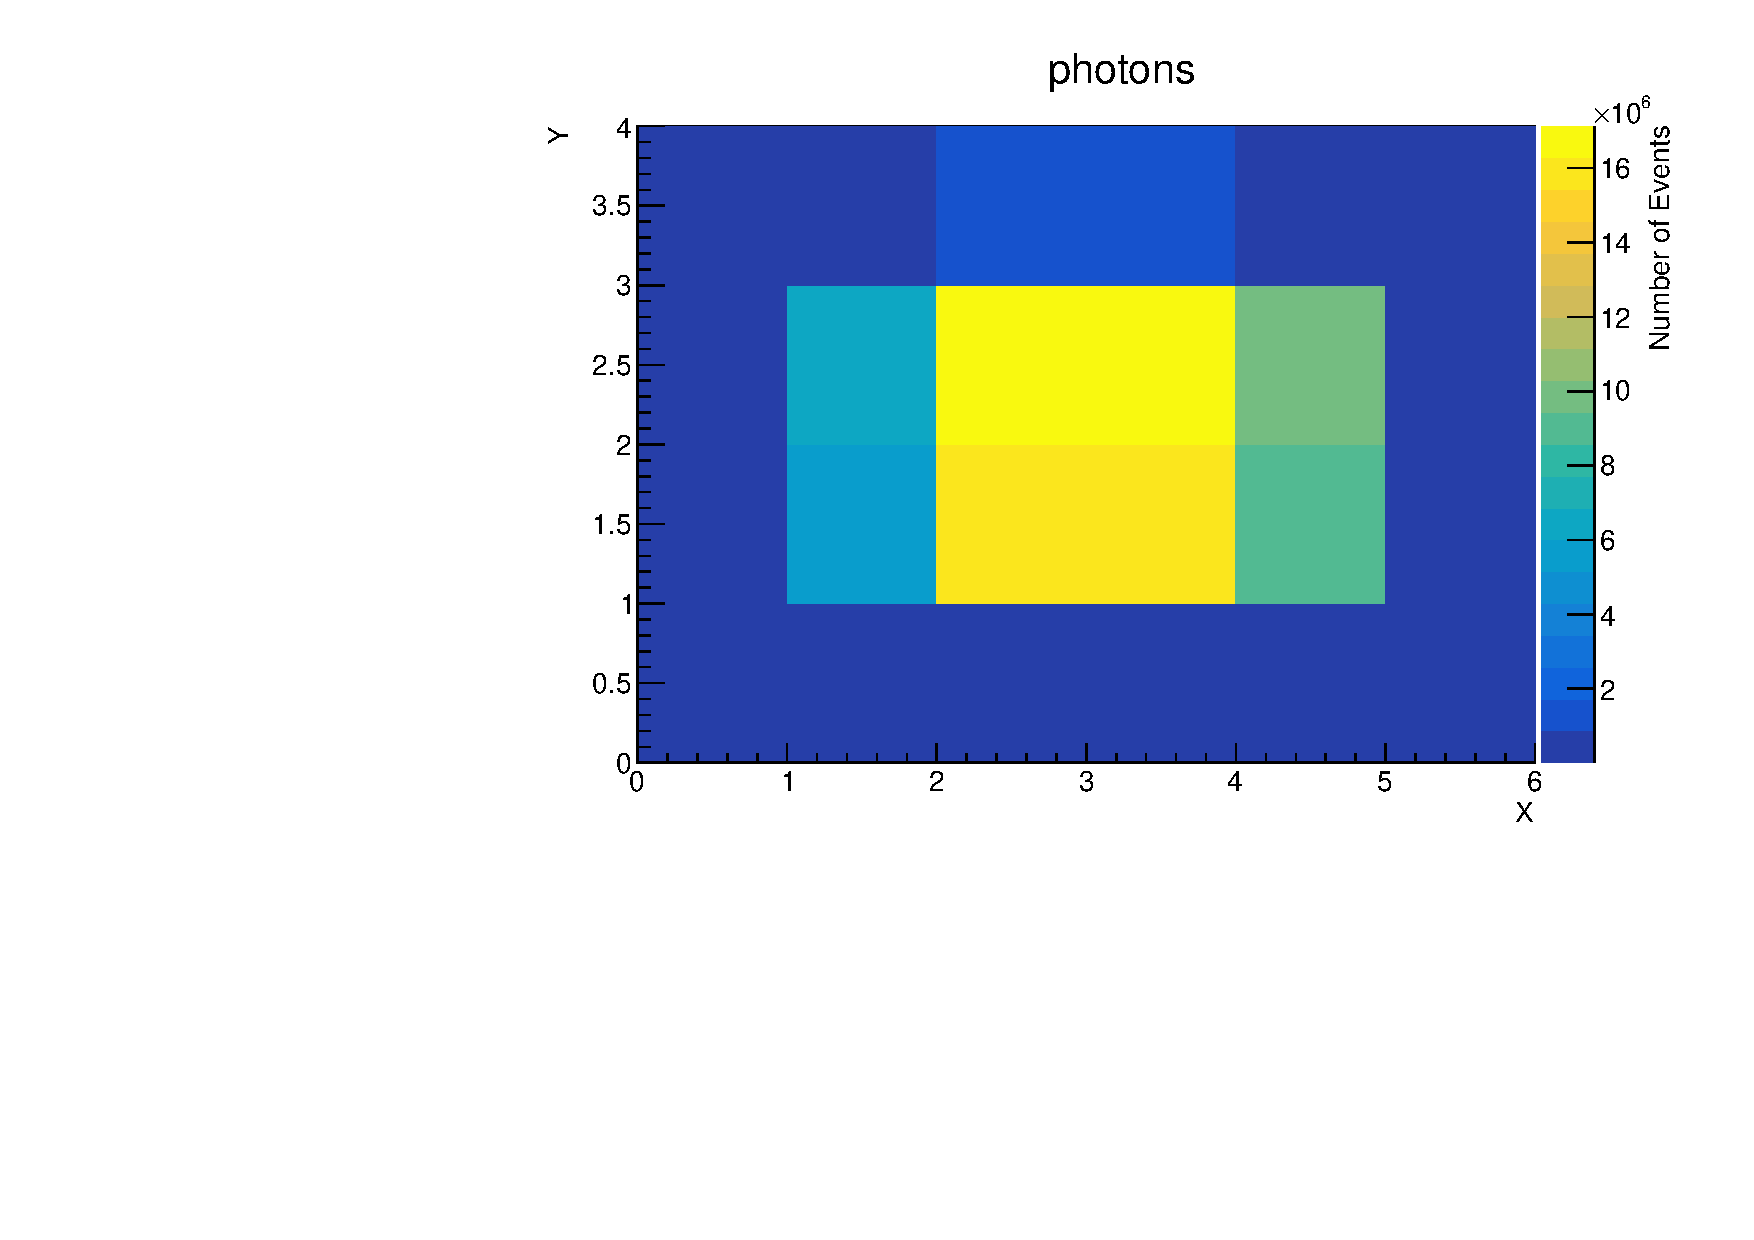
\includegraphics[scale=0.35]{Kap3/electron_lead_photons_plots_calo_counter.pdf}\label{fig:photons-creation-lead-1}}\hspace{1em}
  \subfloat[\(e^-\) as primary particle, Z axis of the calorimeter.]{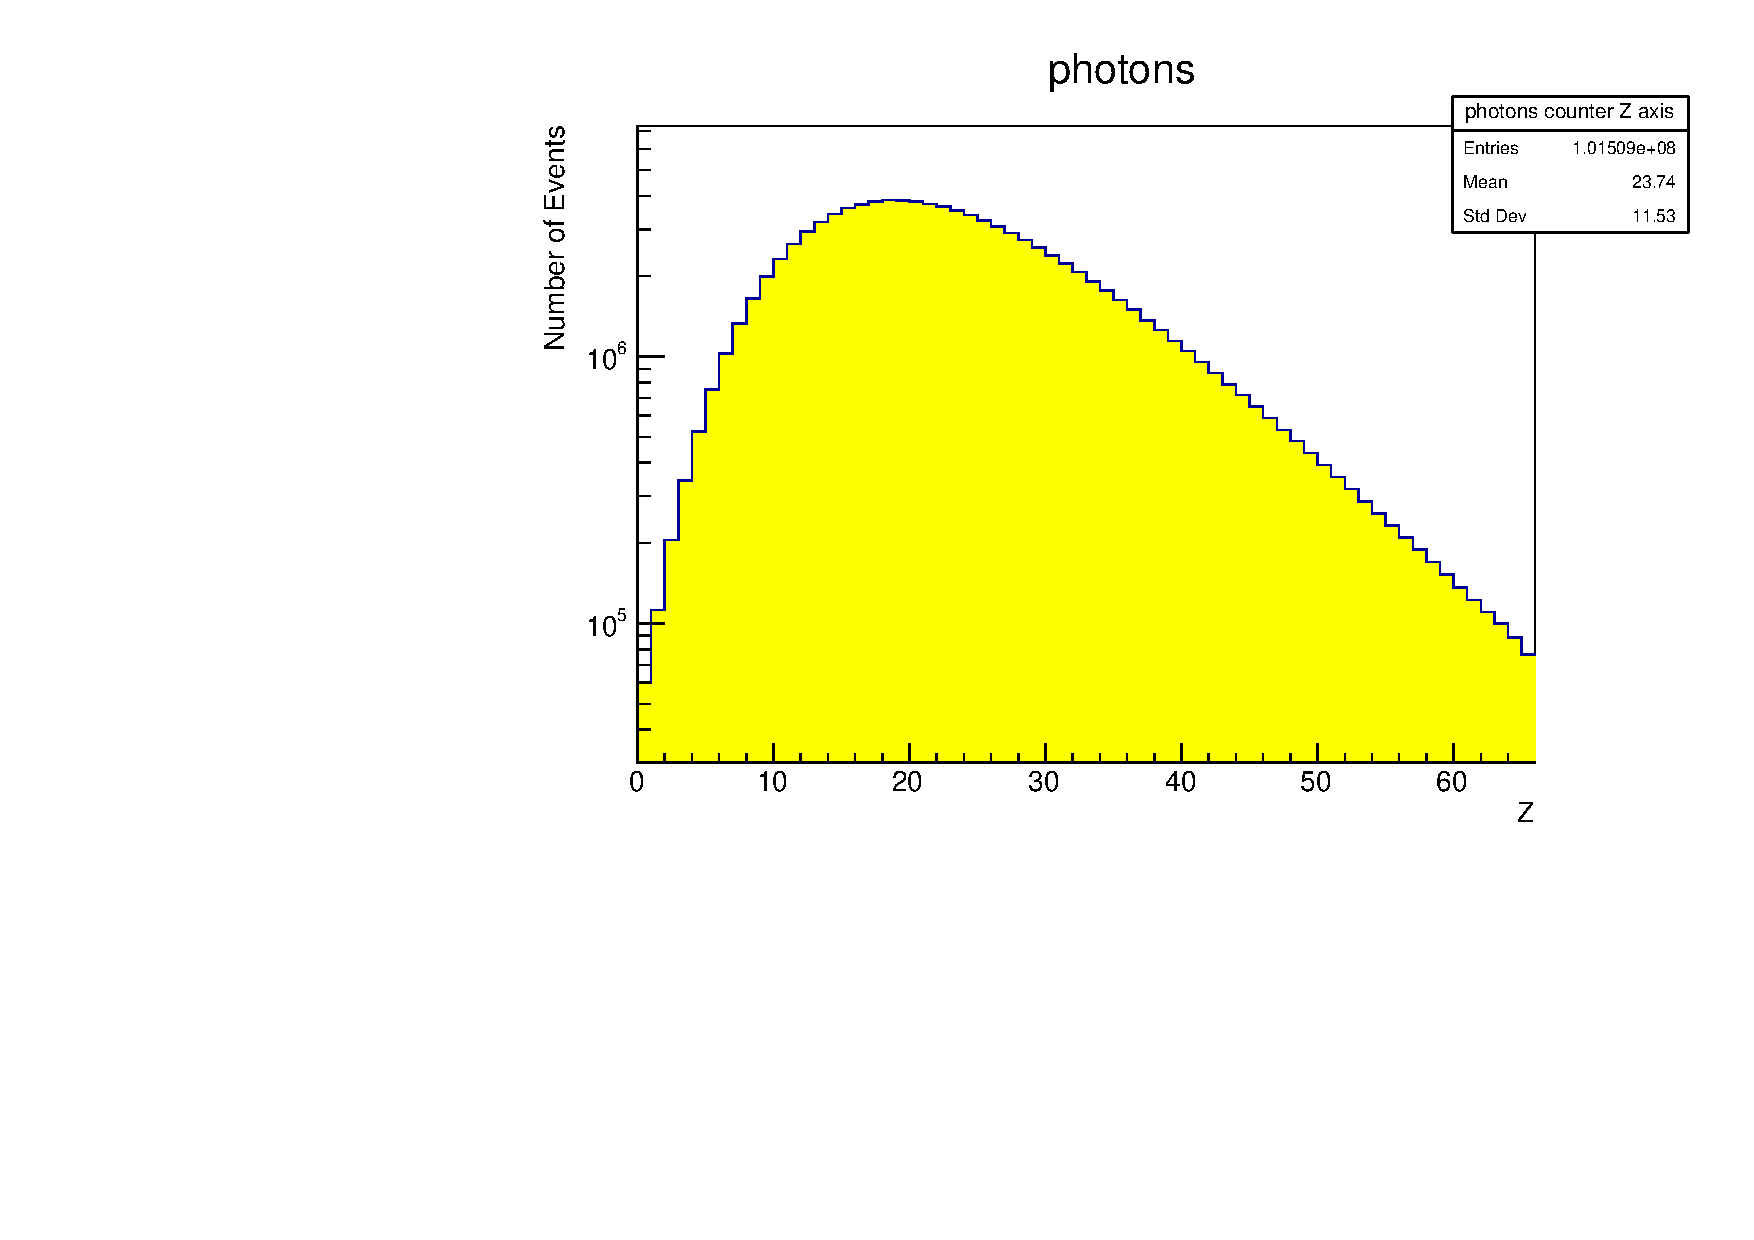
\includegraphics[scale=0.35]{Kap3/electron_lead_photons_plots_calo_counter_Z.pdf}\label{fig:photons-creation-lead-2}}

  \subfloat[\(\gamma\) as primary particle, X-Y plane of the calorimeter.]{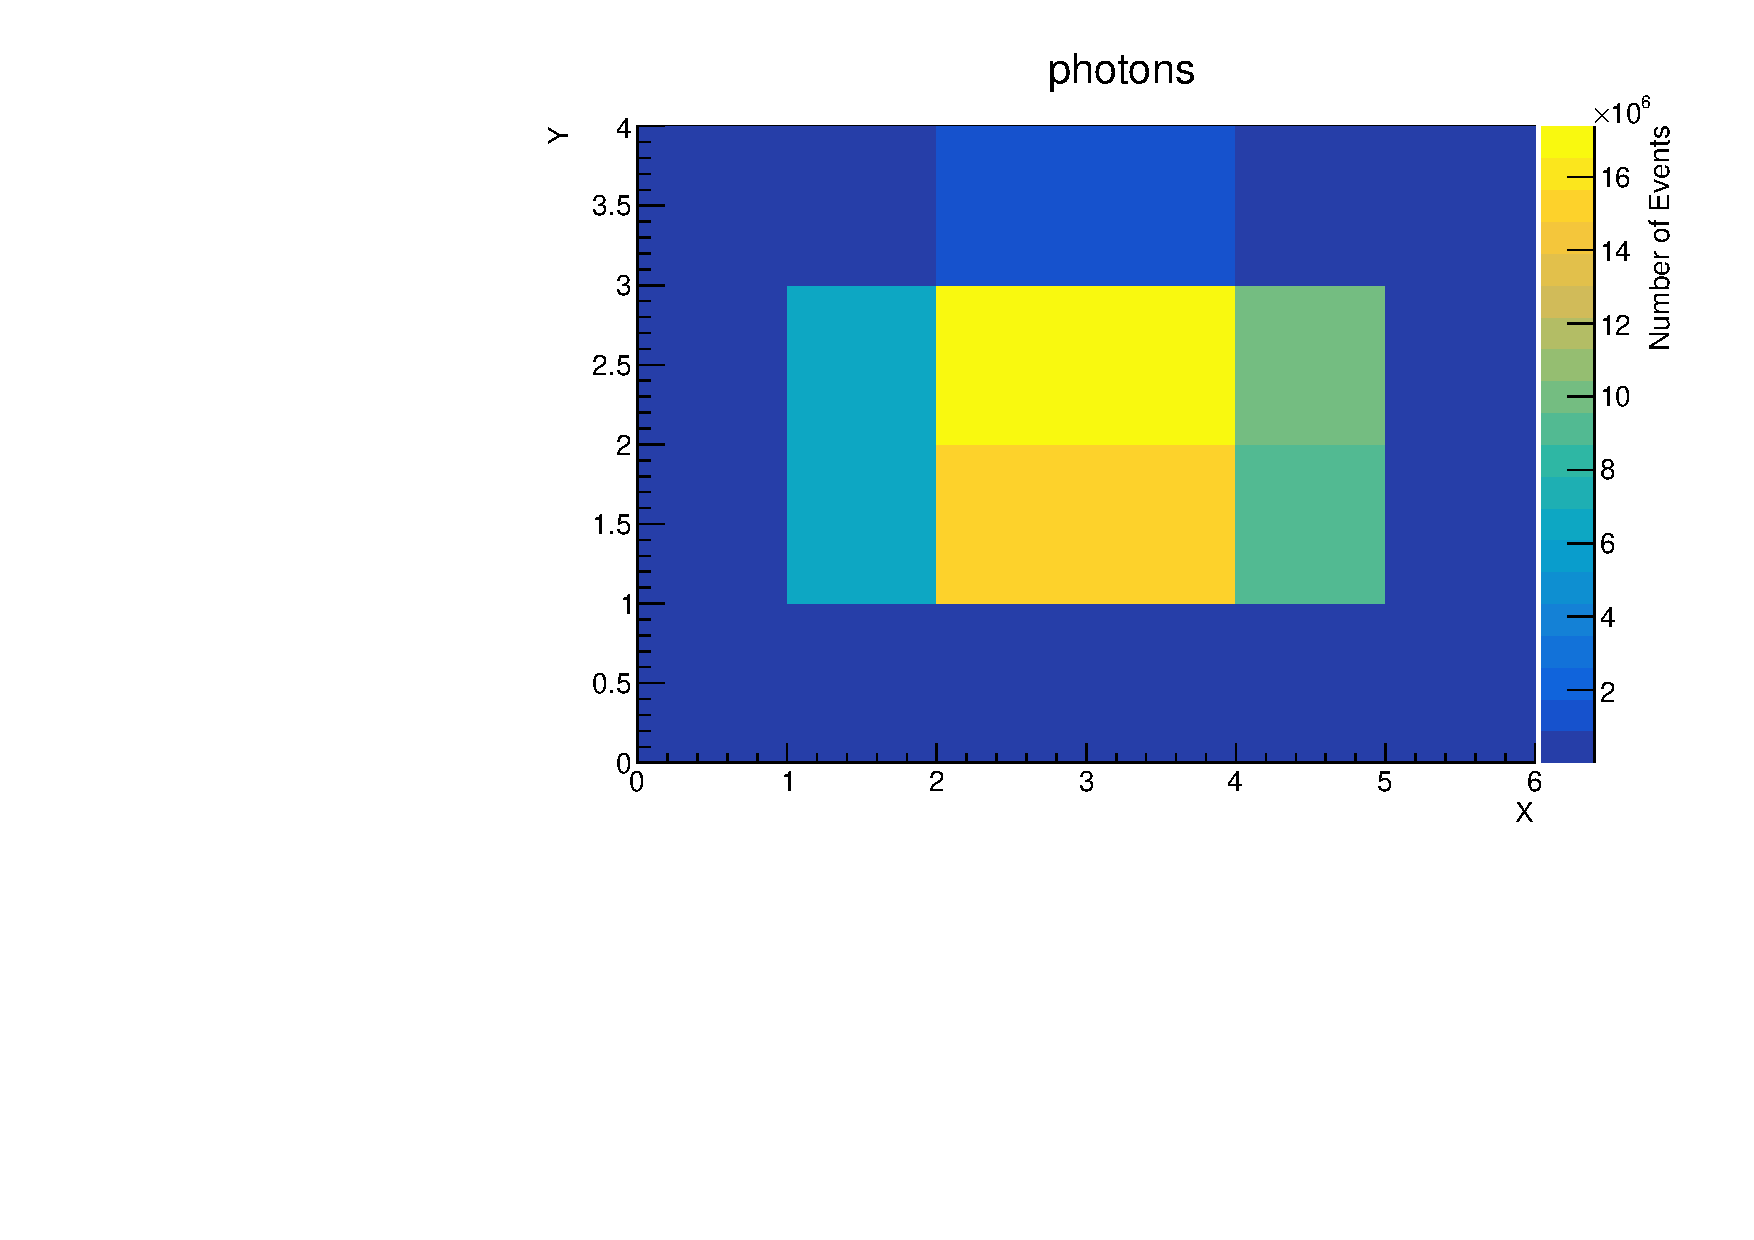
\includegraphics[scale=0.35]{Kap3/gamma_lead_photons_plots_calo_counter.pdf}\label{fig:photons-creation-lead-3}}\hspace{1em}
  \subfloat[\(\gamma\) as primary particle, Z axis of the calorimeter.]{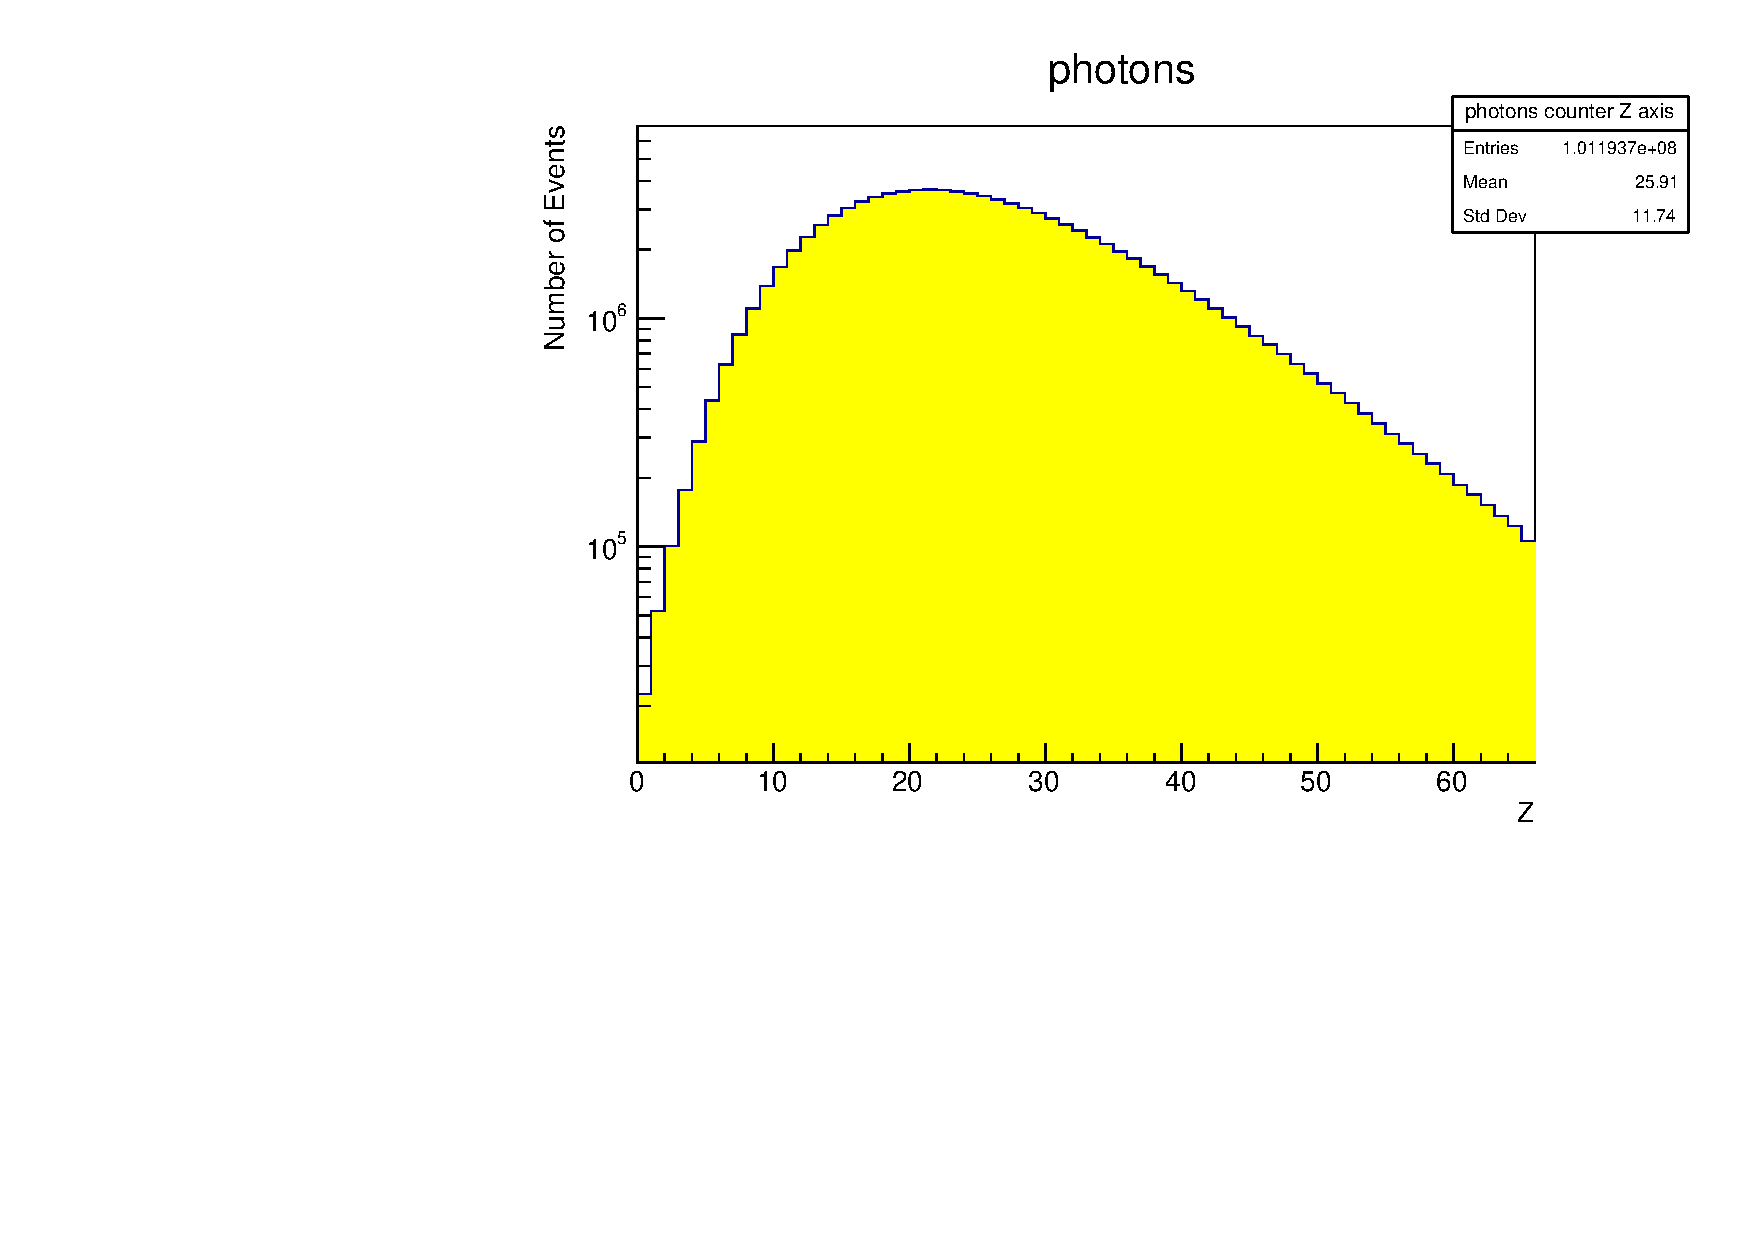
\includegraphics[scale=0.35]{Kap3/gamma_lead_photons_plots_calo_counter_Z.pdf}\label{fig:photons-creation-lead-4}}

  \subfloat[\(\pi^0\) as primary particle, X-Y plane of the calorimeter.]{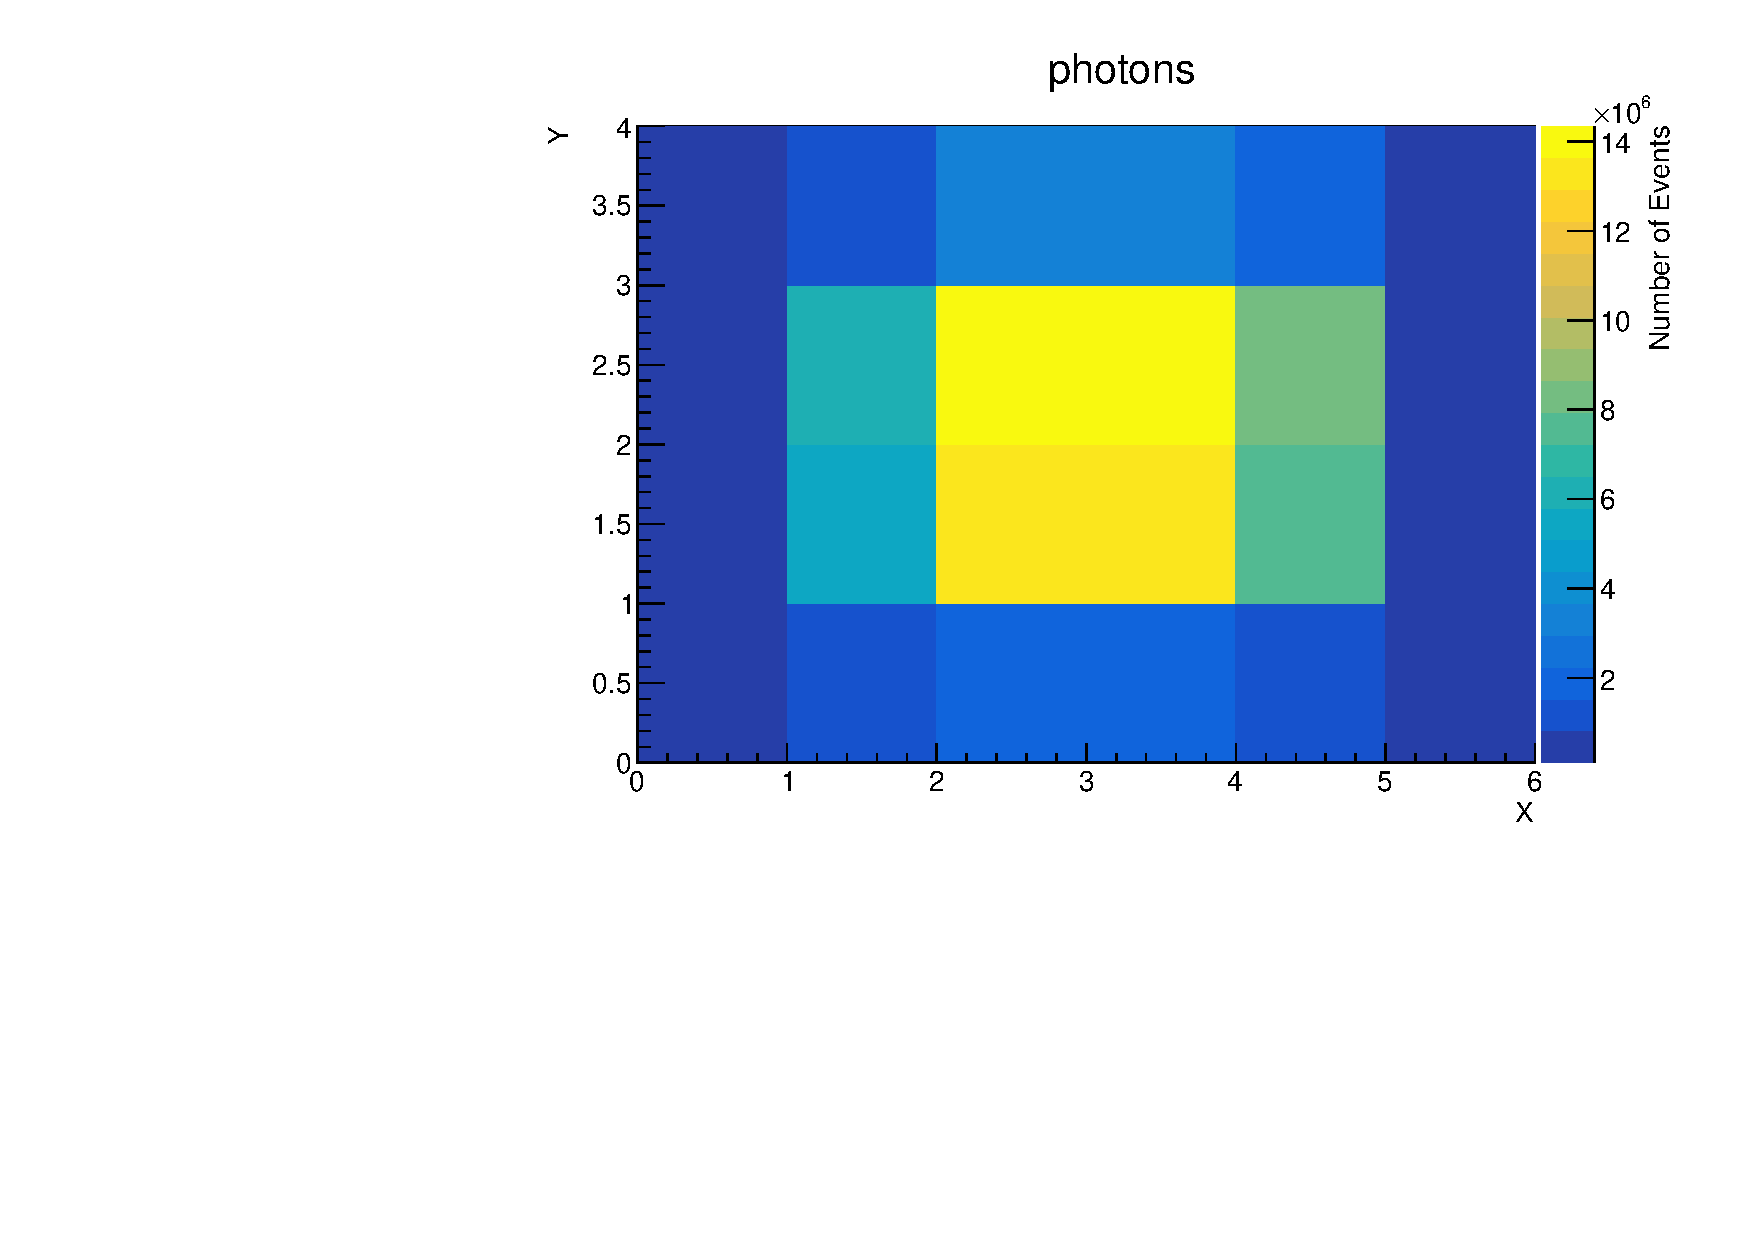
\includegraphics[scale=0.35]{Kap3/pi0_lead_photons_plots_calo_counter.pdf}\label{fig:photons-creation-lead-5}}\hspace{1em}
  \subfloat[\(\pi^0\) as primary particle, Z axis of the calorimeter.]{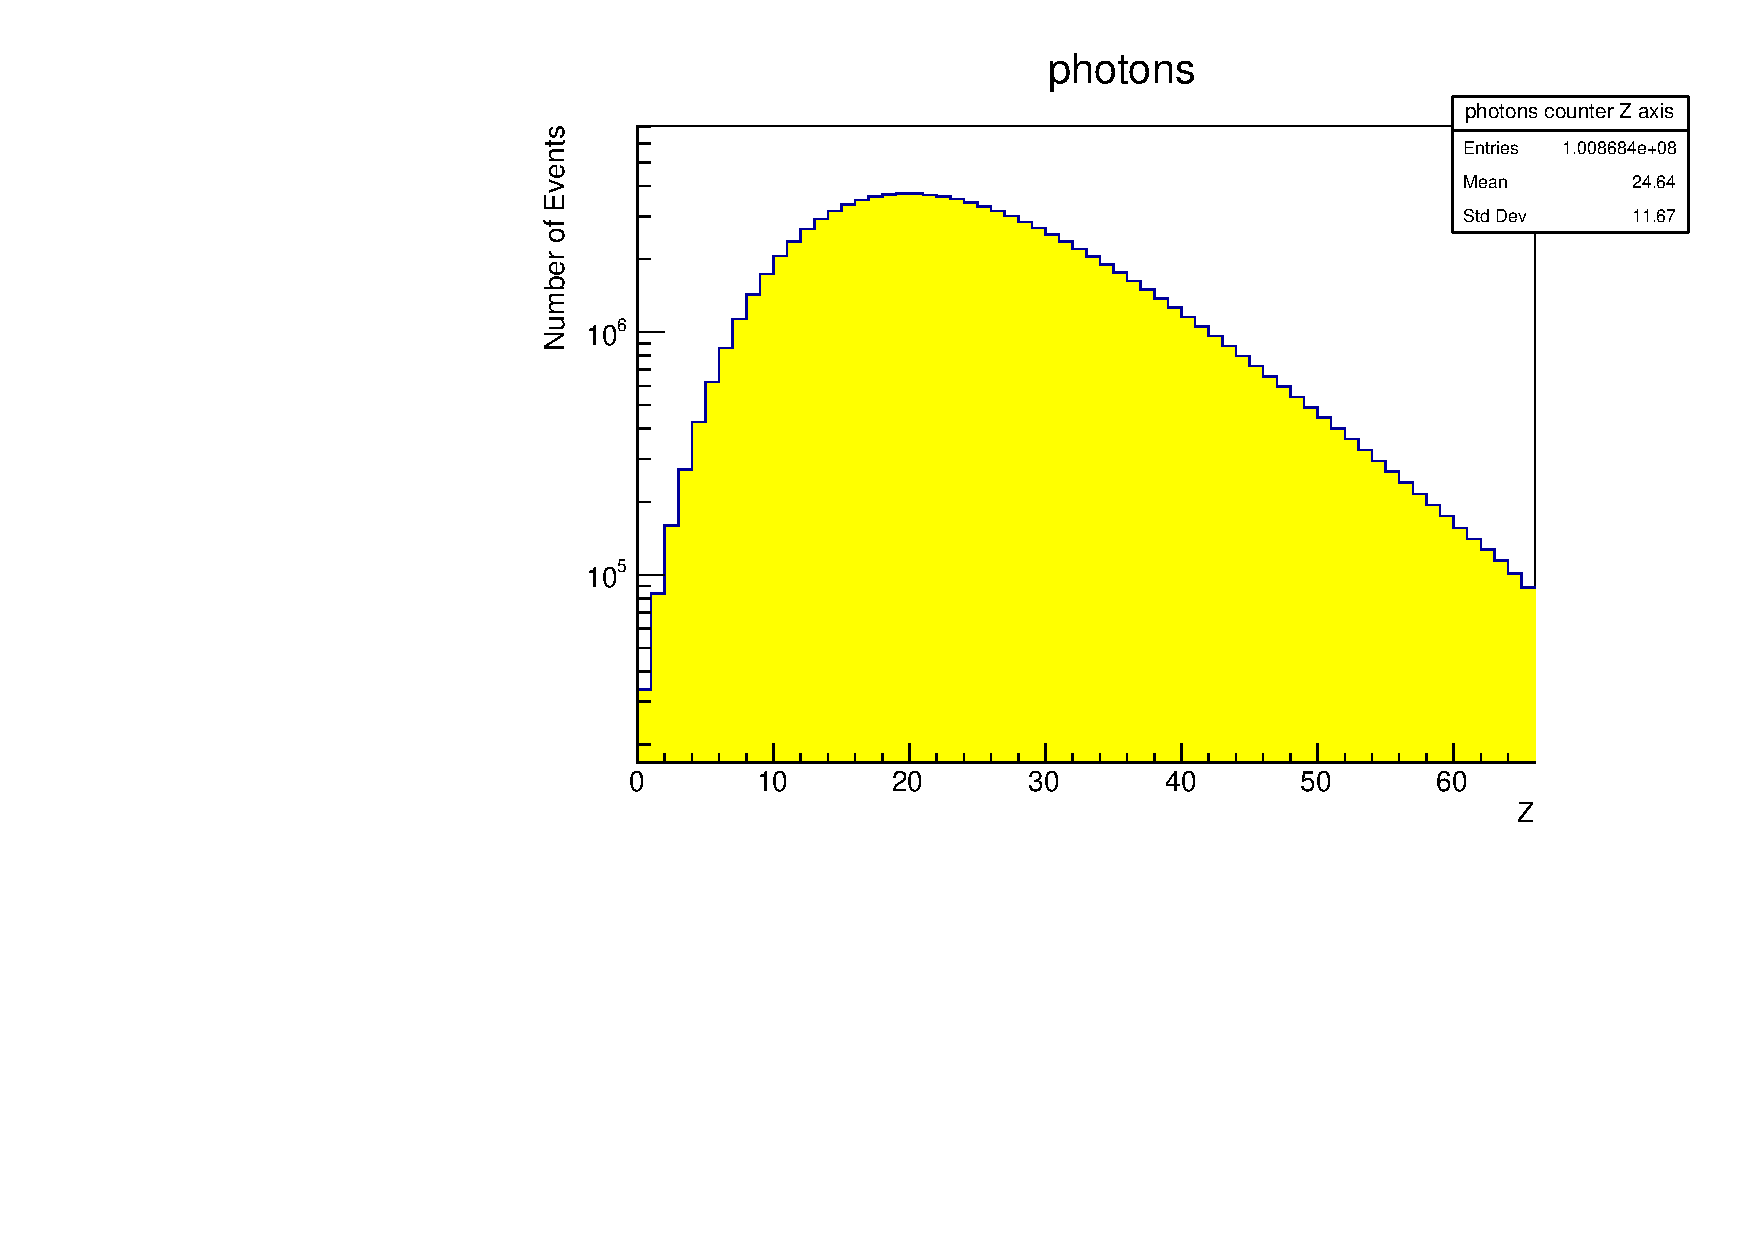
\includegraphics[scale=0.35]{Kap3/pi0_lead_photons_plots_calo_counter_Z.pdf}\label{fig:photons-creation-lead-6}}

  \caption{Photons creation in the lead plates of the calorimeter.}\label{fig:photons-creation-lead}

\end{figure}

For both electron and protons, the distribution in the Z axis did not show
significant differences, the mean values are very close one from each other,
however it is to mention that in the two cases, the lowest mean value is when
the primary particle is an electron, and the greatest when it is a photon.

In the case of the particle production in the lead, the main value is again in
the central zone of the detector, and also, the standard deviations in the
pions signal is larger. For the photon creation, shown in the
\cref{fig:photons-creation-lead}, the standard deviation of the electrons,
photons and pions are \((0.949, 0.584)\), \((0.951, 0.583)\) and \((1.028,
0.758)\) respectively.

\begin{figure}[htb!]
  \centering

  \subfloat[\(e^-\) as primary particle, X-Y plane of the calorimeter.]{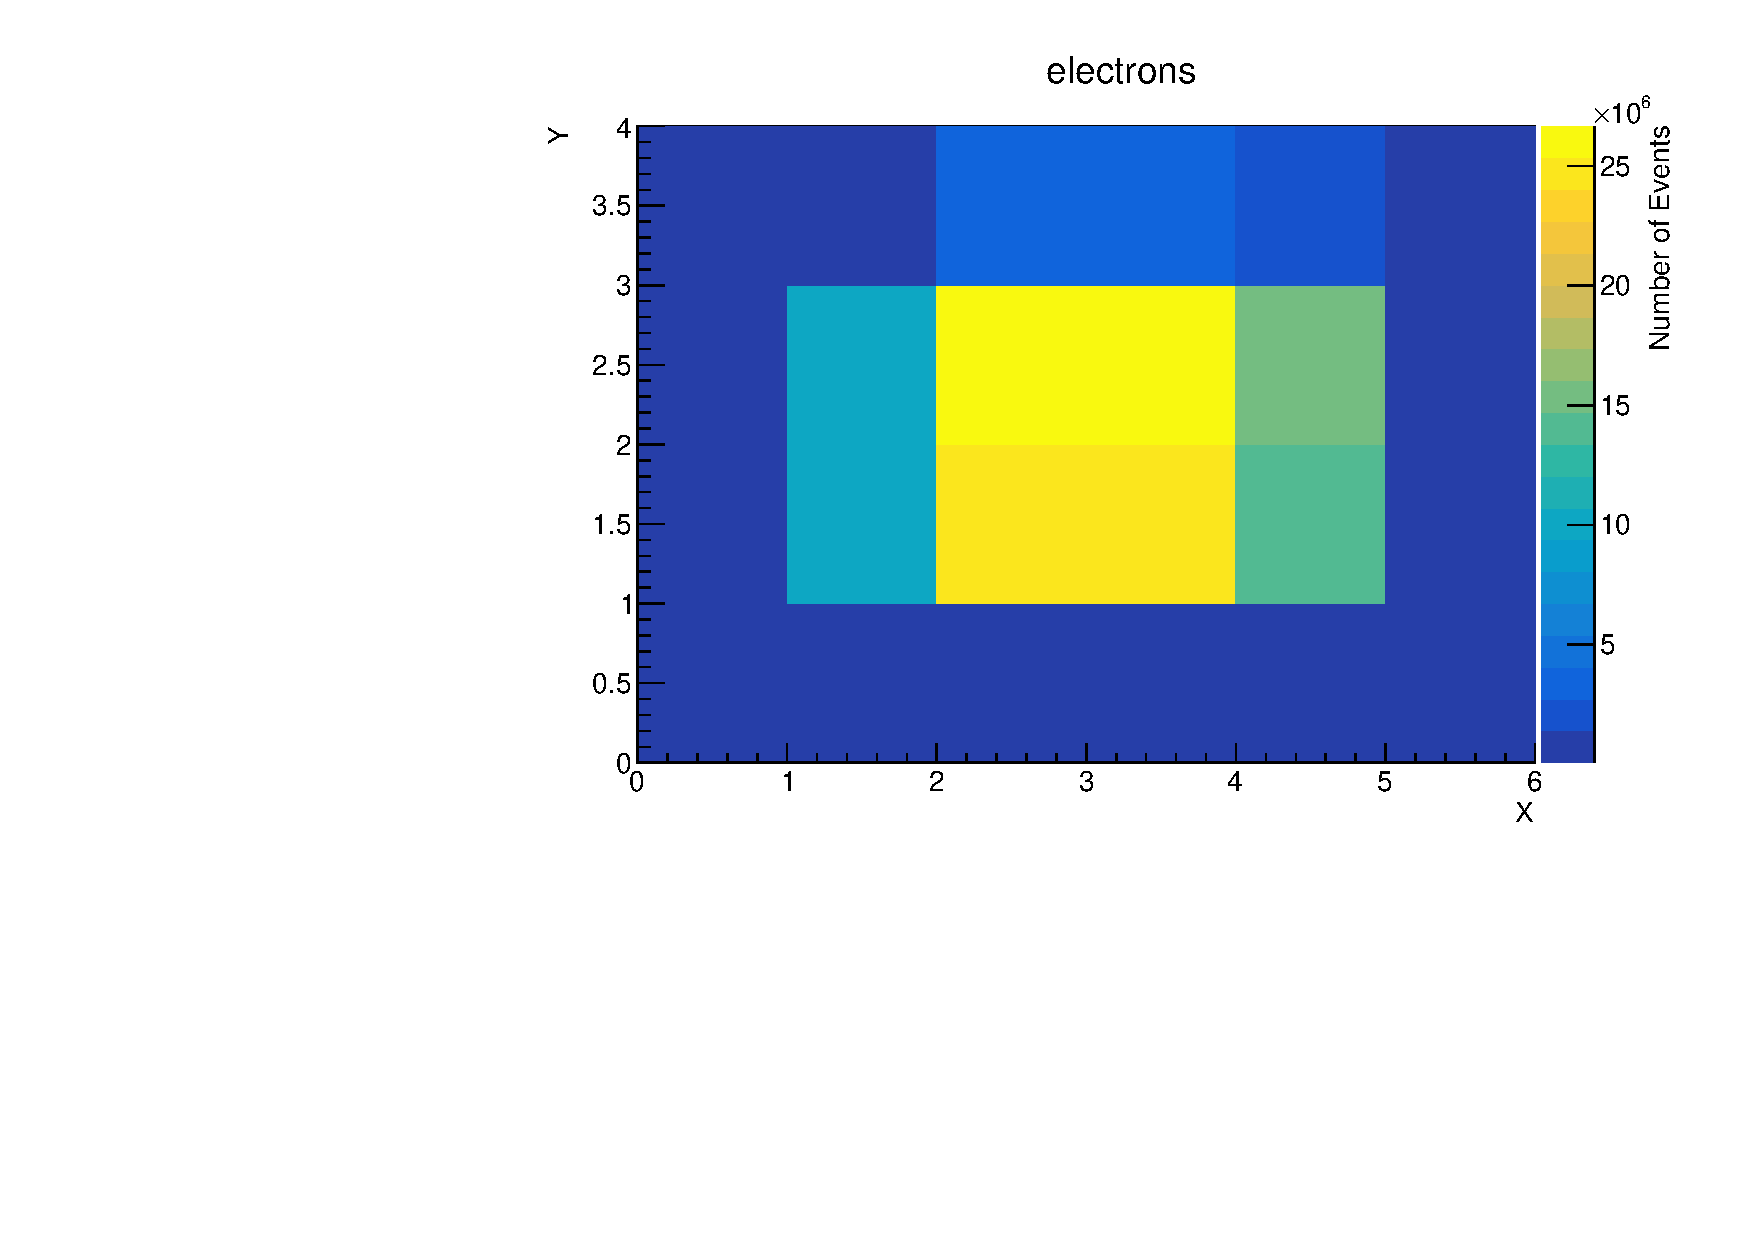
\includegraphics[scale=0.35]{Kap3/electron_lead_electrons_plots_calo_counter.pdf}\label{fig:electrons-creation-lead-1}}\hspace{1em}
  \subfloat[\(e^-\) as primary particle, Z axis of the calorimeter.]{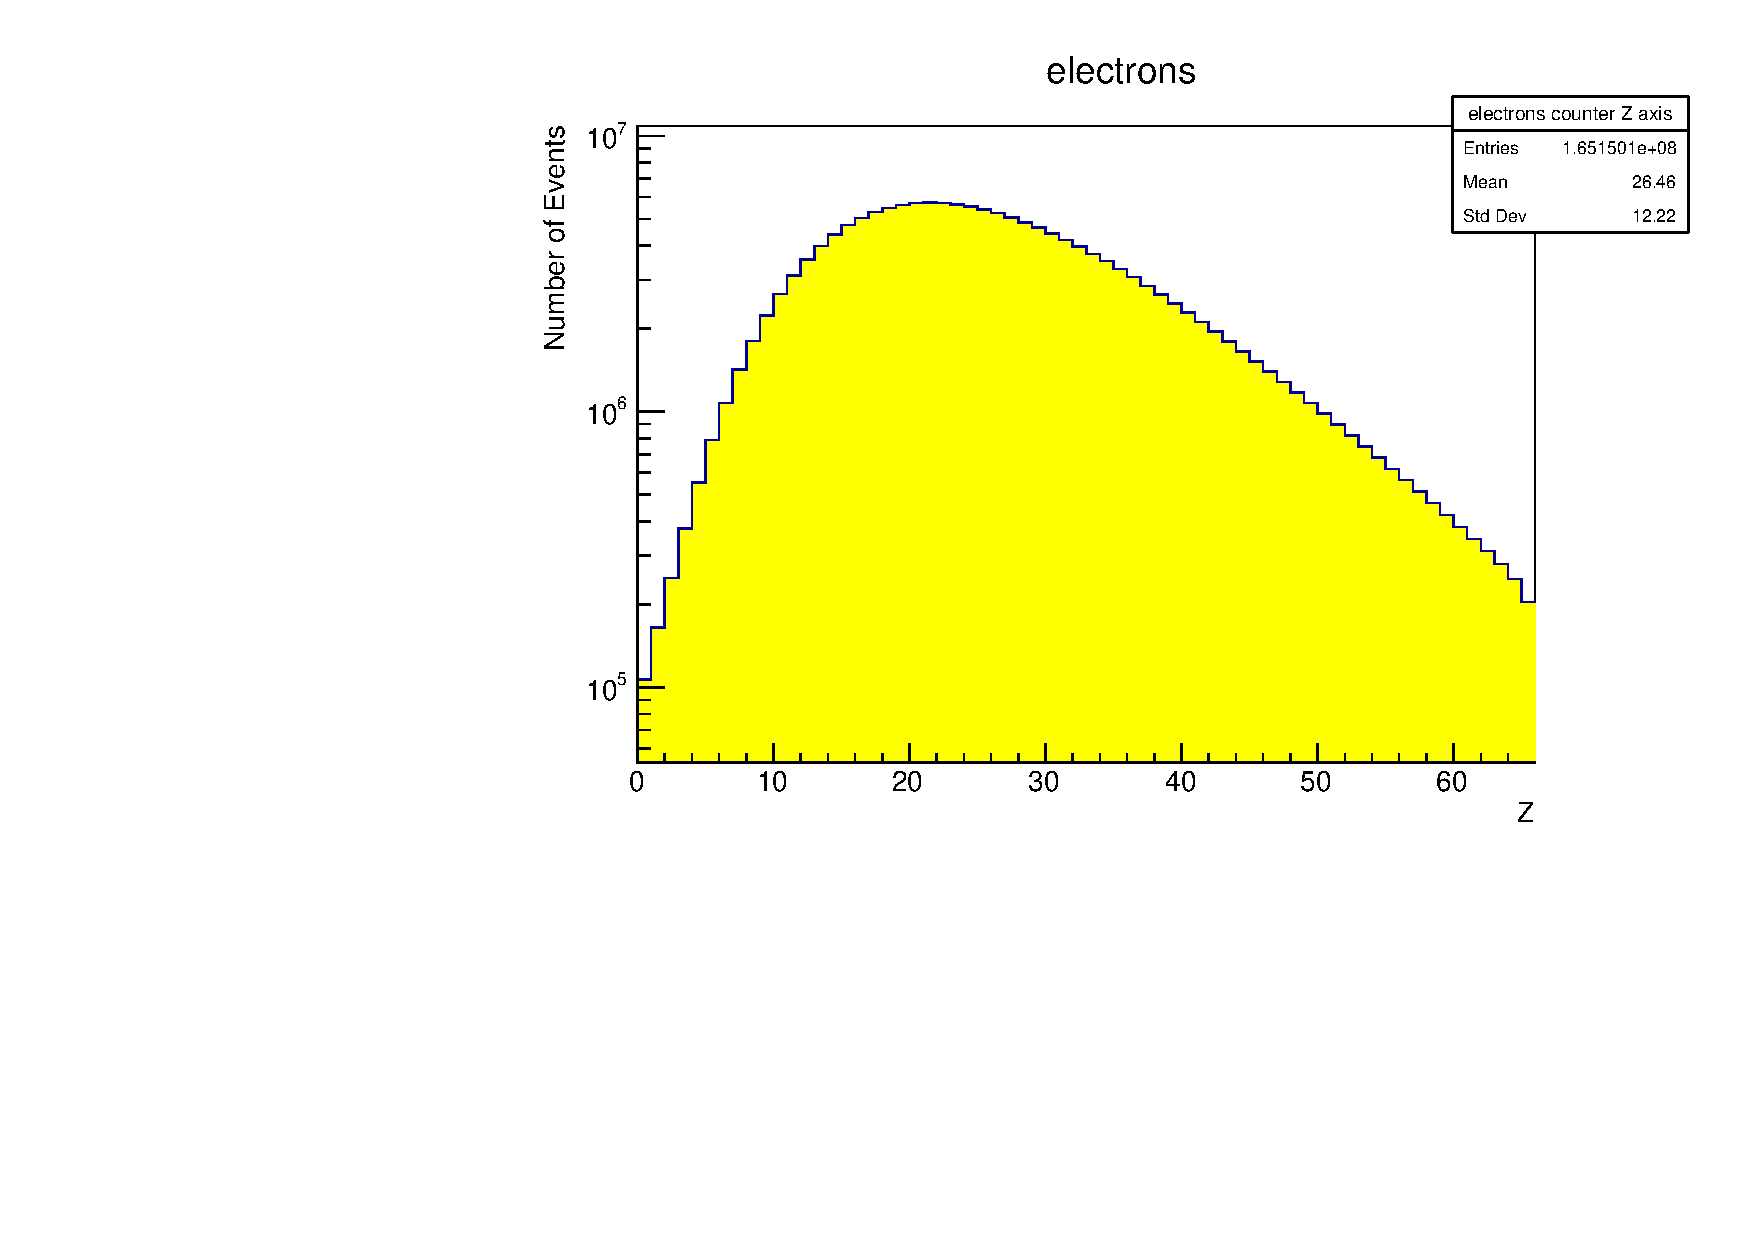
\includegraphics[scale=0.35]{Kap3/electron_lead_electrons_plots_calo_counter_Z.pdf}\label{fig:electrons-creation-lead-2}}

  \subfloat[\(\gamma\) as primary particle, X-Y plane of the calorimeter.]{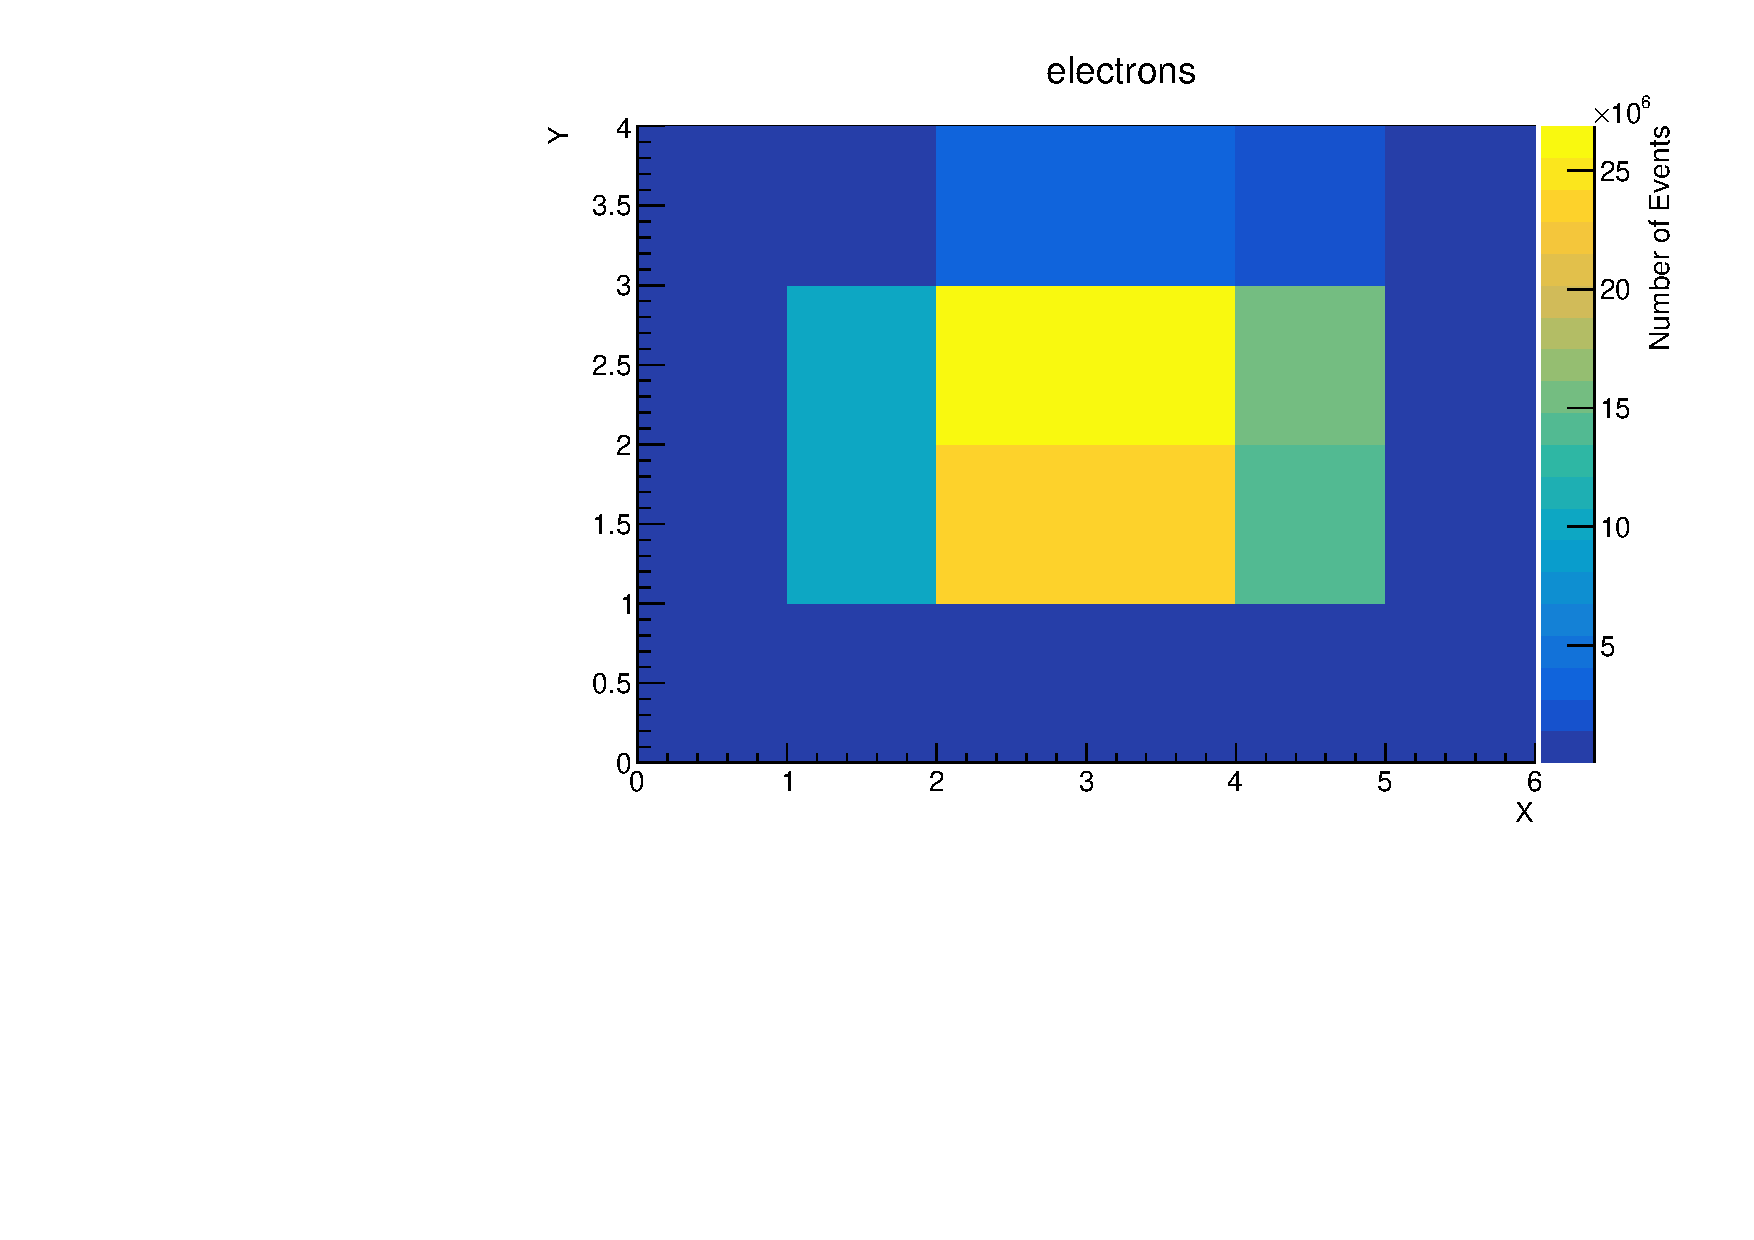
\includegraphics[scale=0.35]{Kap3/gamma_lead_electrons_plots_calo_counter.pdf}\label{fig:electrons-creation-lead-3}}\hspace{1em}
  \subfloat[\(\gamma\) as primary particle, Z axis of the calorimeter.]{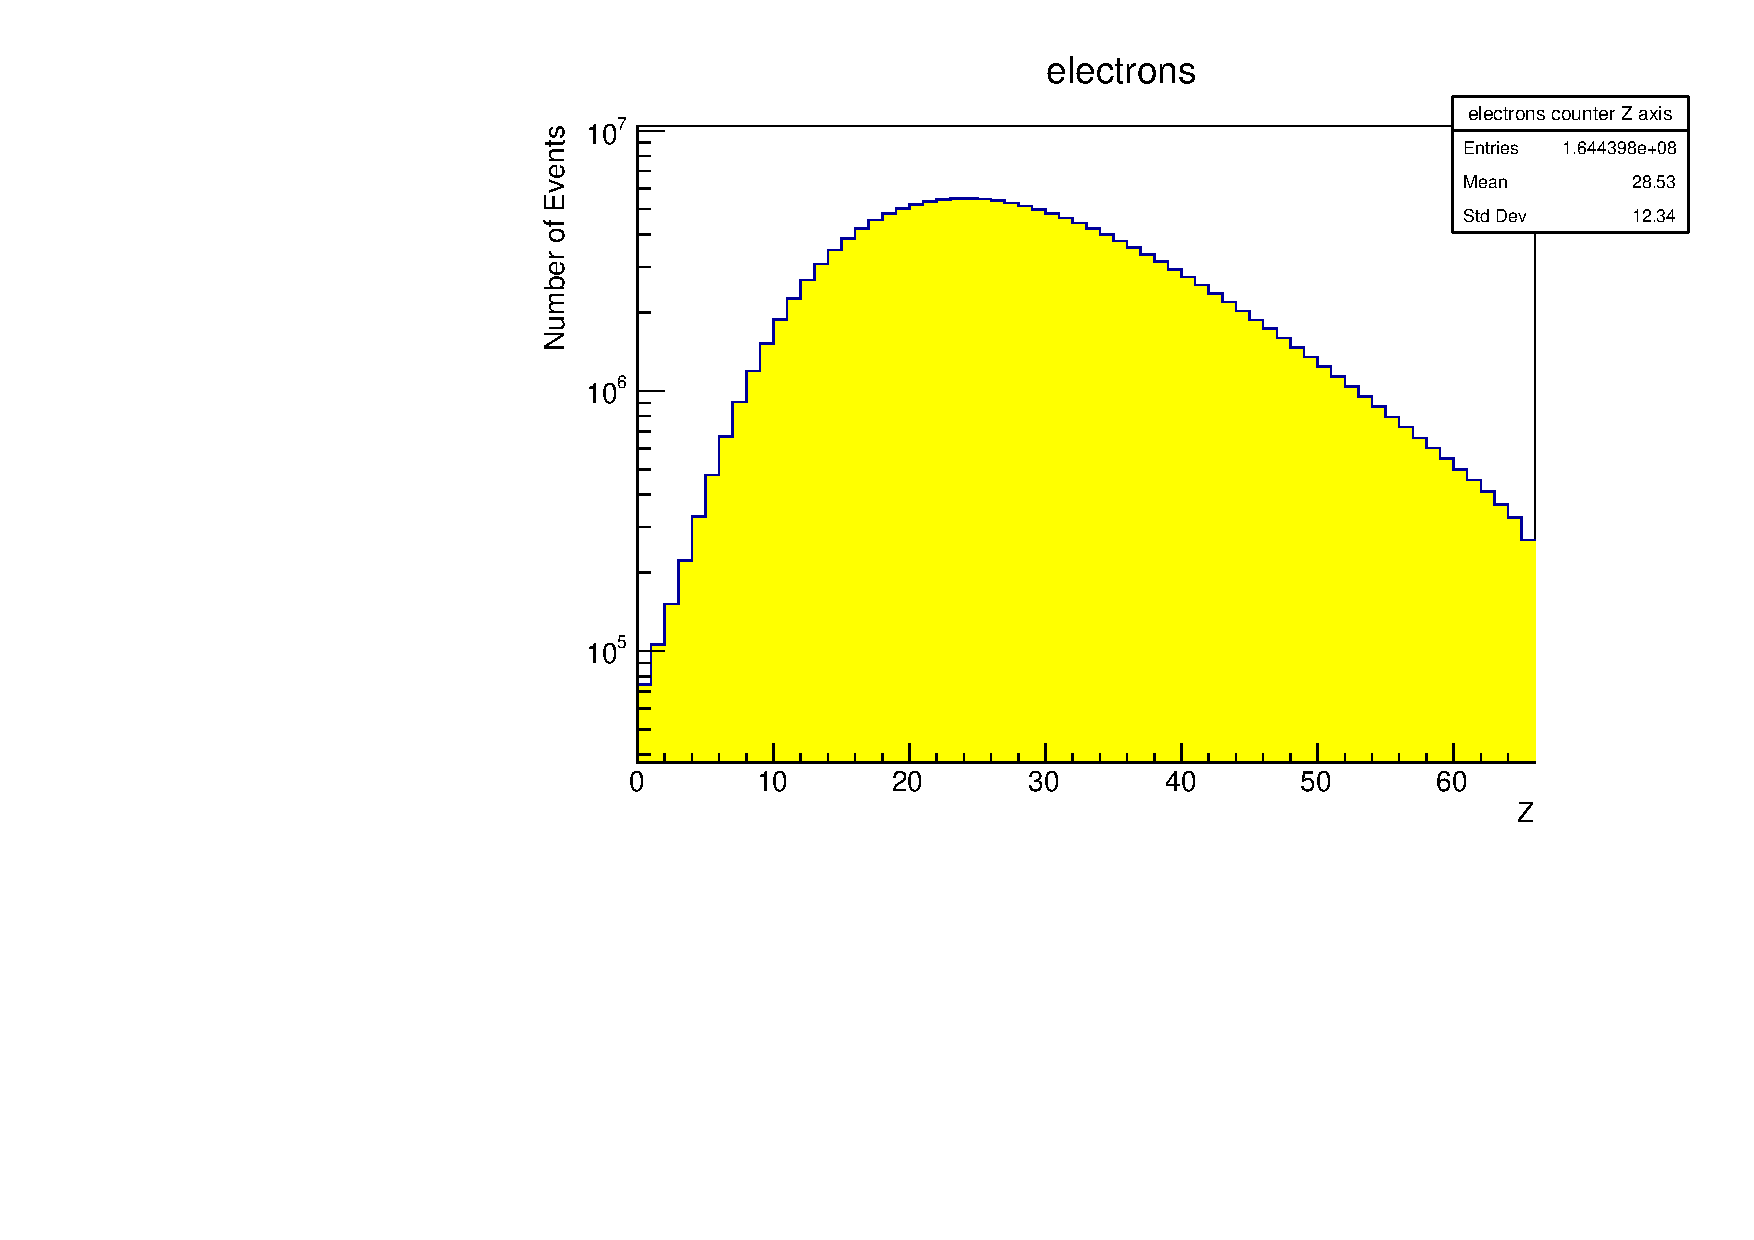
\includegraphics[scale=0.35]{Kap3/gamma_lead_electrons_plots_calo_counter_Z.pdf}\label{fig:electrons-creation-lead-4}}

  \subfloat[\(\pi^0\) as primary particle, X-Y plane of the calorimeter.]{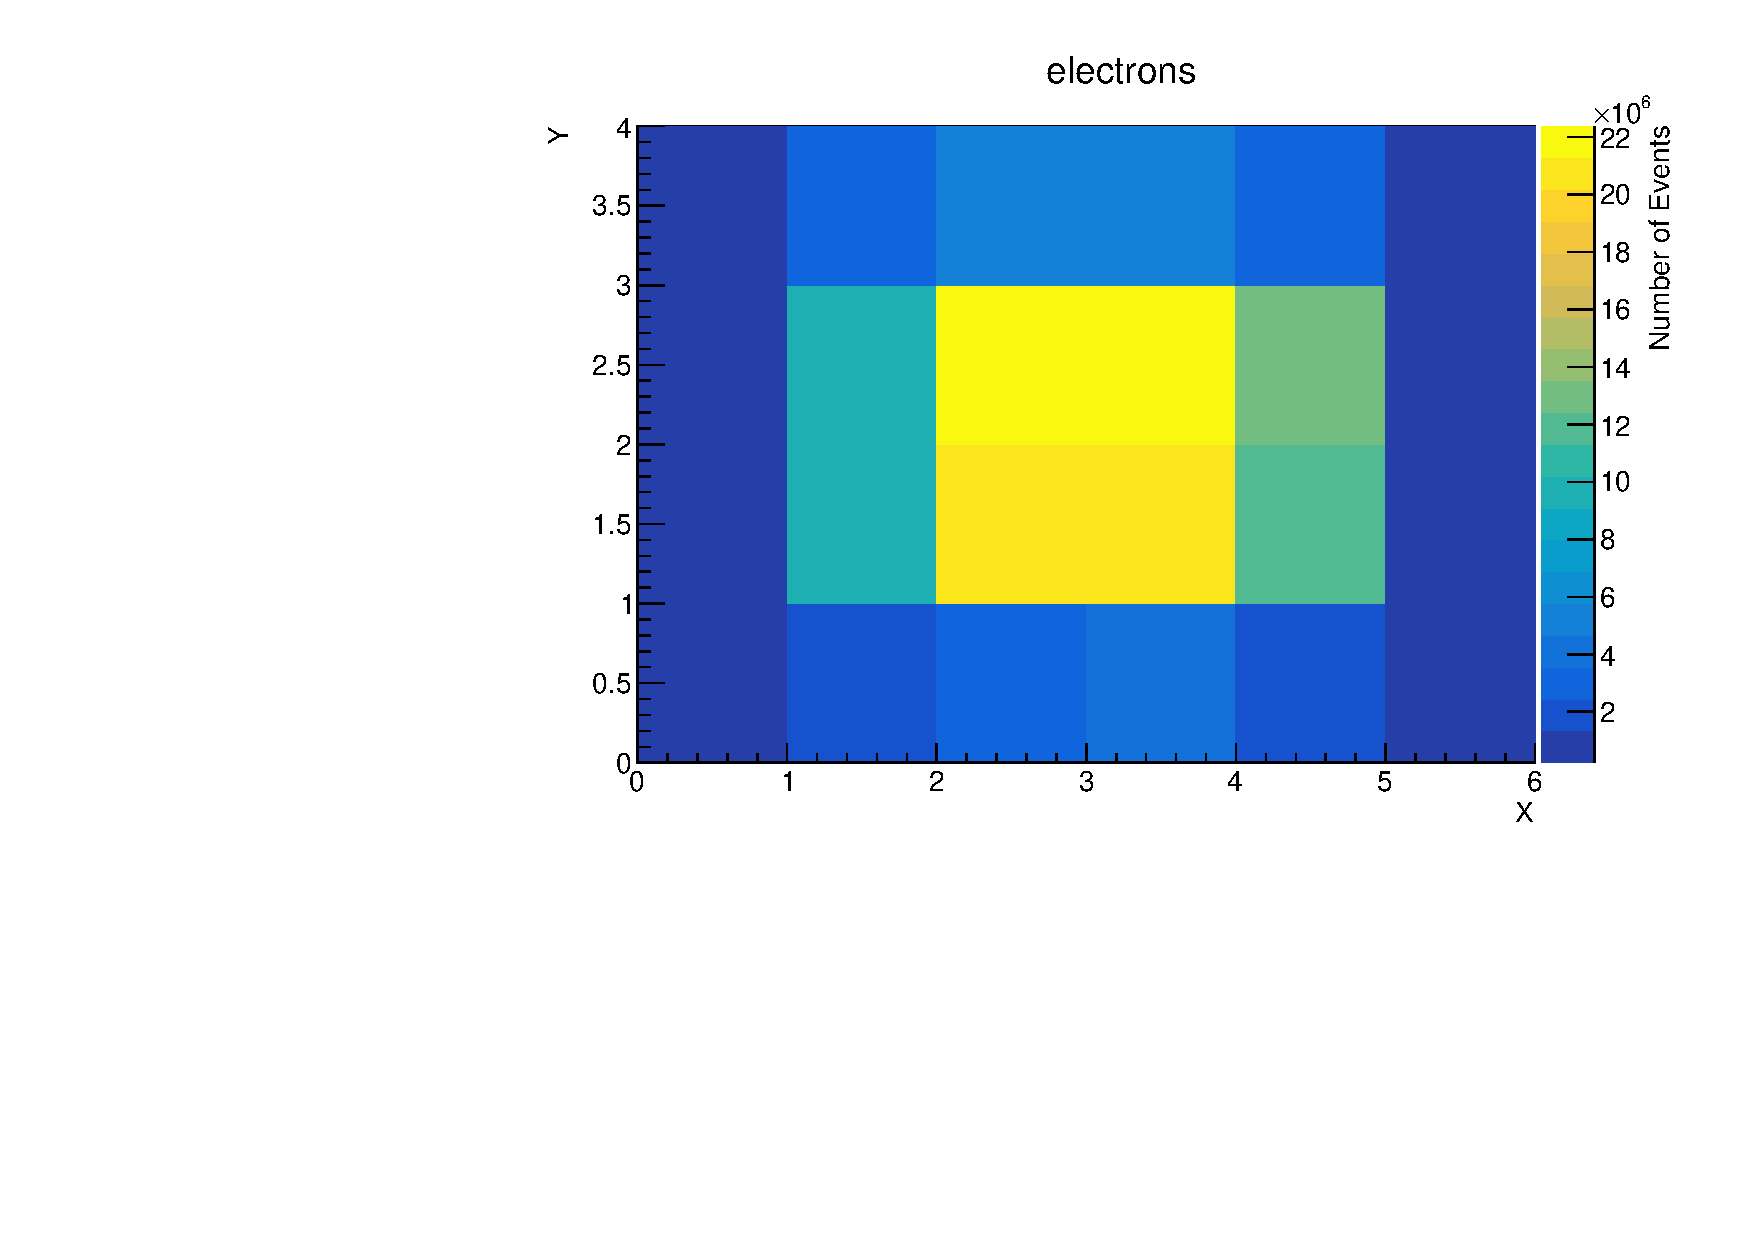
\includegraphics[scale=0.35]{Kap3/pi0_lead_electrons_plots_calo_counter.pdf}\label{fig:electrons-creation-lead-5}}\hspace{1em}
  \subfloat[\(\pi^0\) as primary particle, Z axis of the calorimeter.]{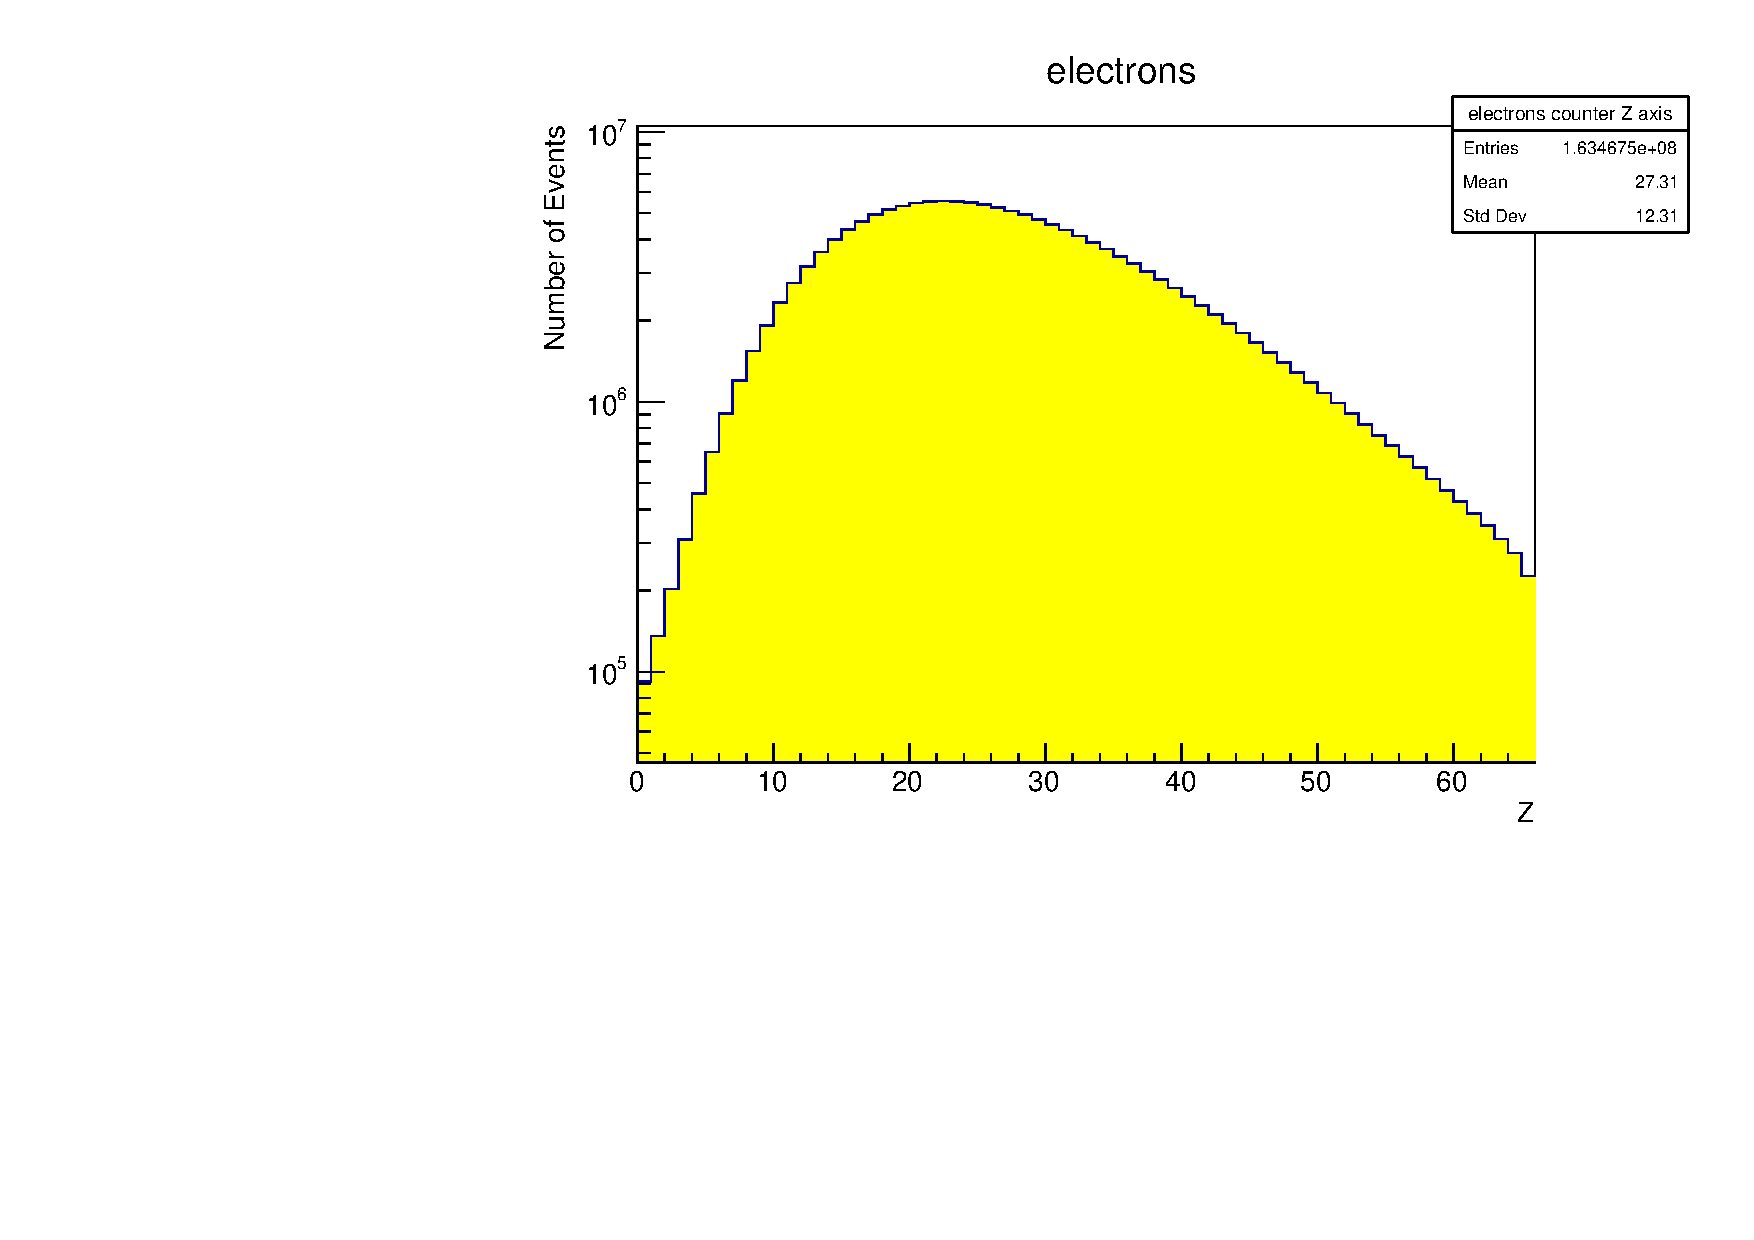
\includegraphics[scale=0.35]{Kap3/pi0_lead_electrons_plots_calo_counter_Z.pdf}\label{fig:electrons-creation-lead-6}}


  \caption{Electron creation in the lead plates of the calorimeter.}\label{fig:electrons-creation-lead}


\end{figure}

For the electron creation as illustrated in \cref{fig:electrons-creation-lead},
the standard deviation for electrons, photons and pions are \((0.9663,
0.6340)\), \((0.9668, 0.6346)\) and \((1.047, 0.7789)\) respectively. Again,
the standard deviation for the neutral pions if large.

\begin{figure}[htb!]
  \centering

  \subfloat[\(e^-\) as primary particle.]{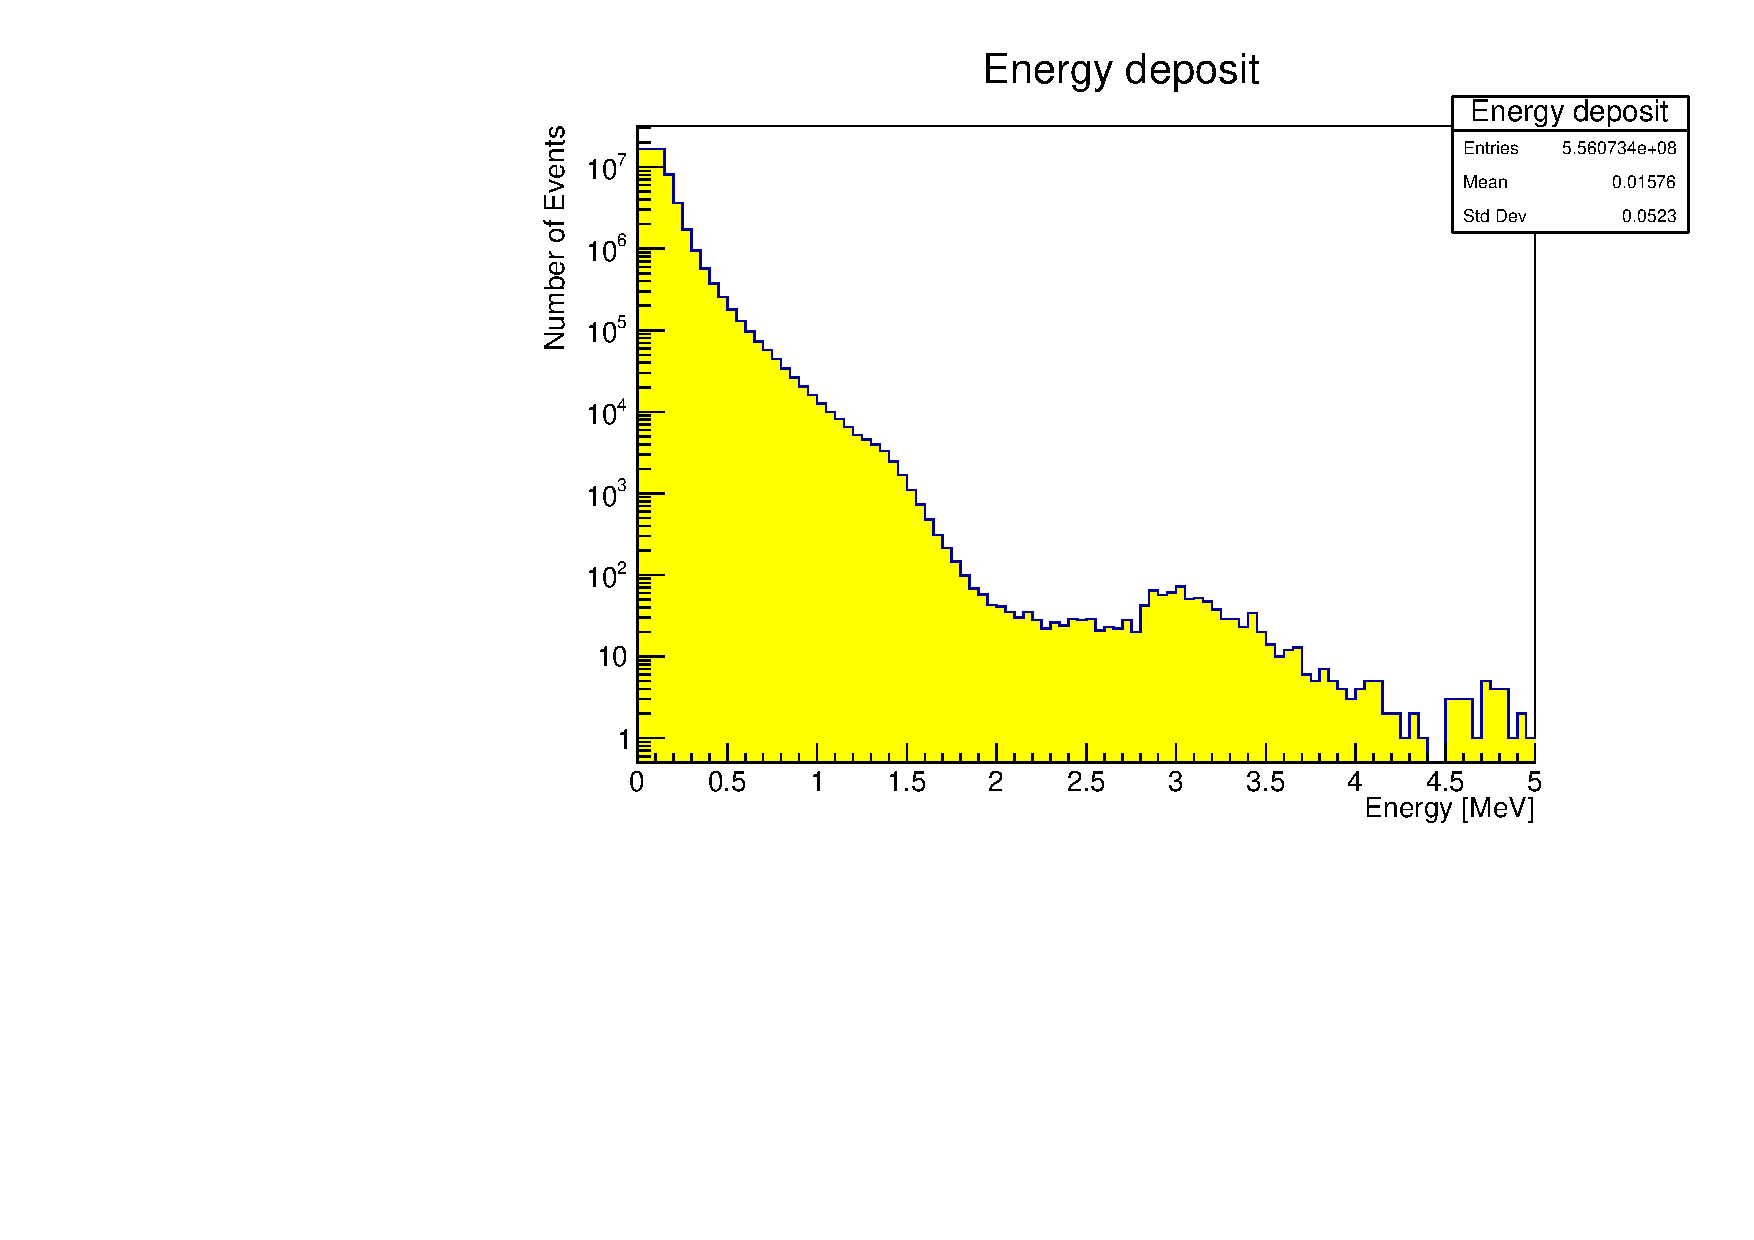
\includegraphics[scale=0.35]{Kap3/electron_scintillator_electrons_plots_energy_hist.pdf}\label{fig:energy-scintillator-1}}\hspace{1em}
  \subfloat[\(\gamma\) as primary particle.]{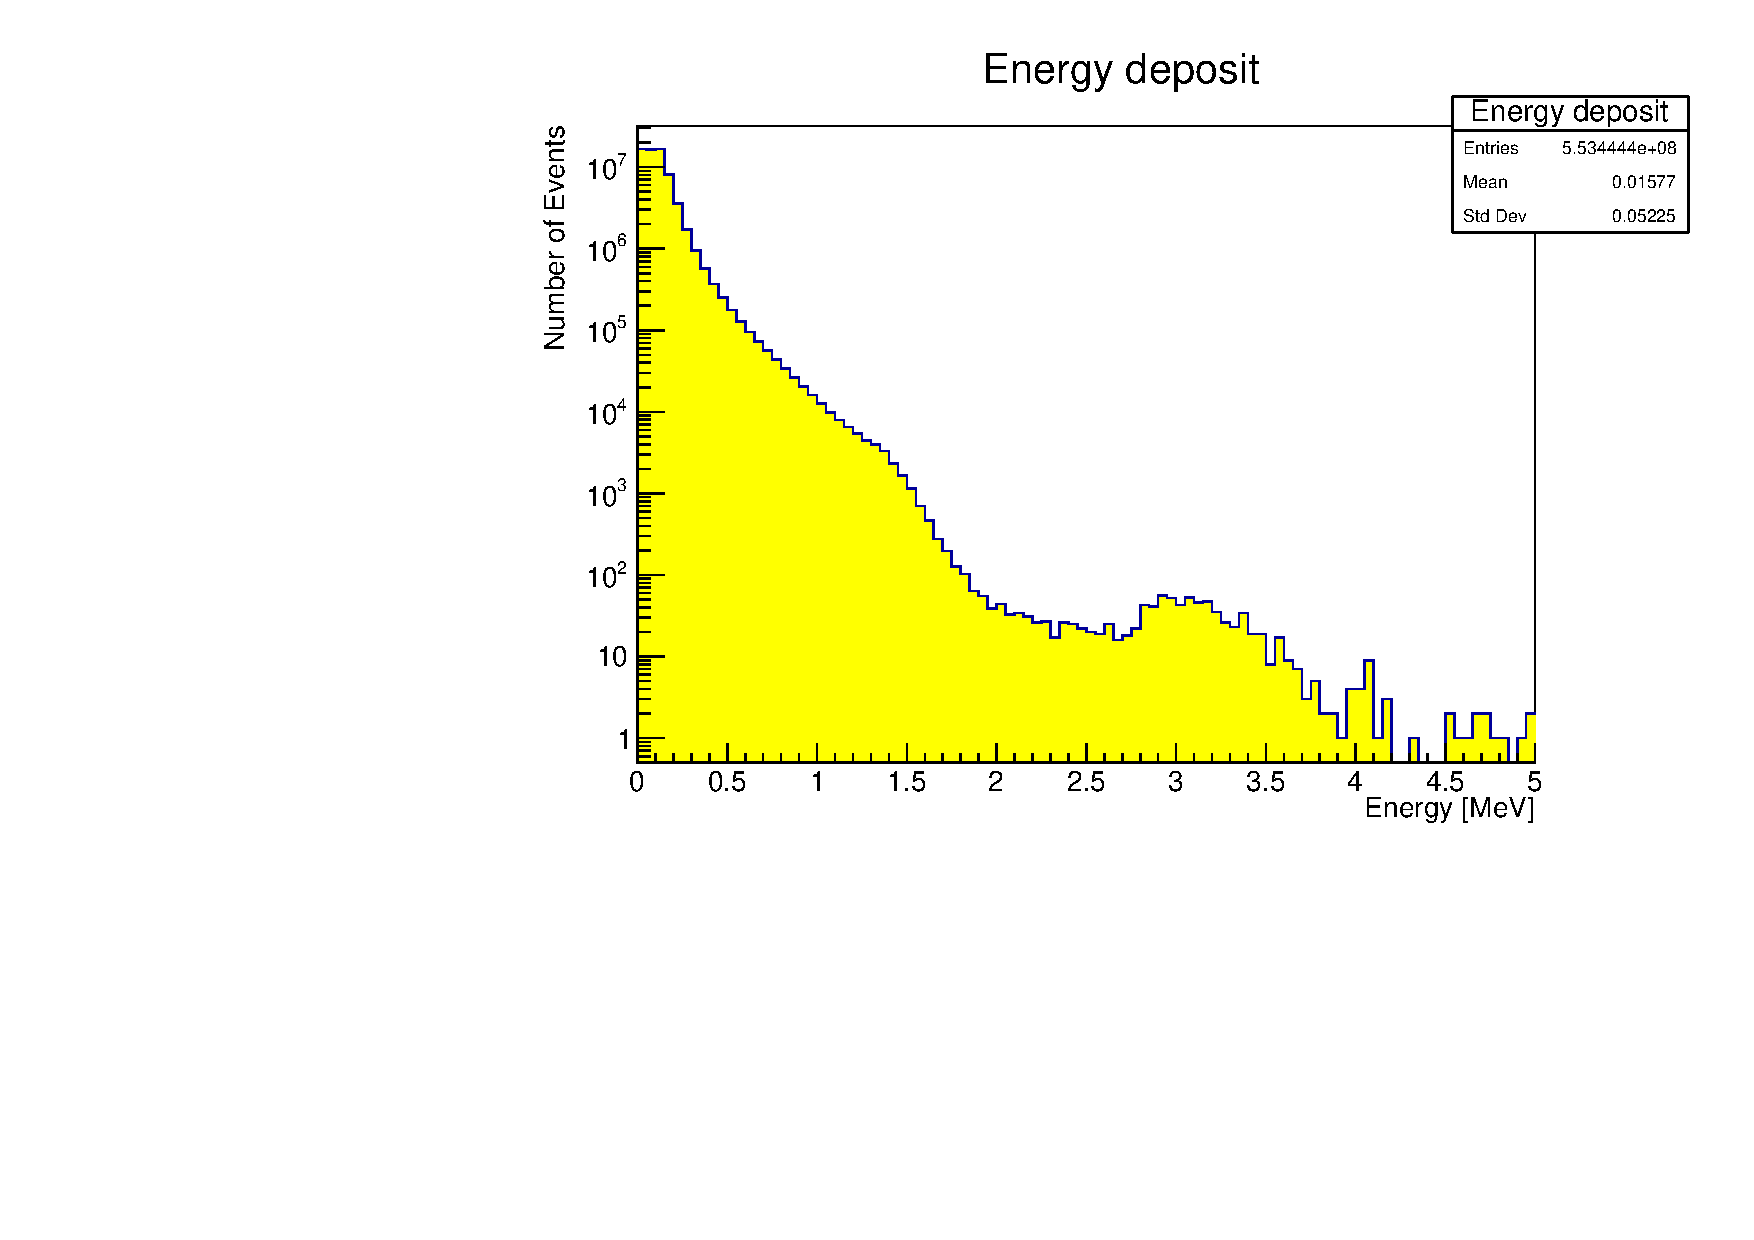
\includegraphics[scale=0.35]{Kap3/gamma_scintillator_electrons_plots_energy_hist.pdf}\label{fig:energy-scintillator-2}}\hspace{1em}
  \subfloat[\(\pi^0\) as primary particle.]{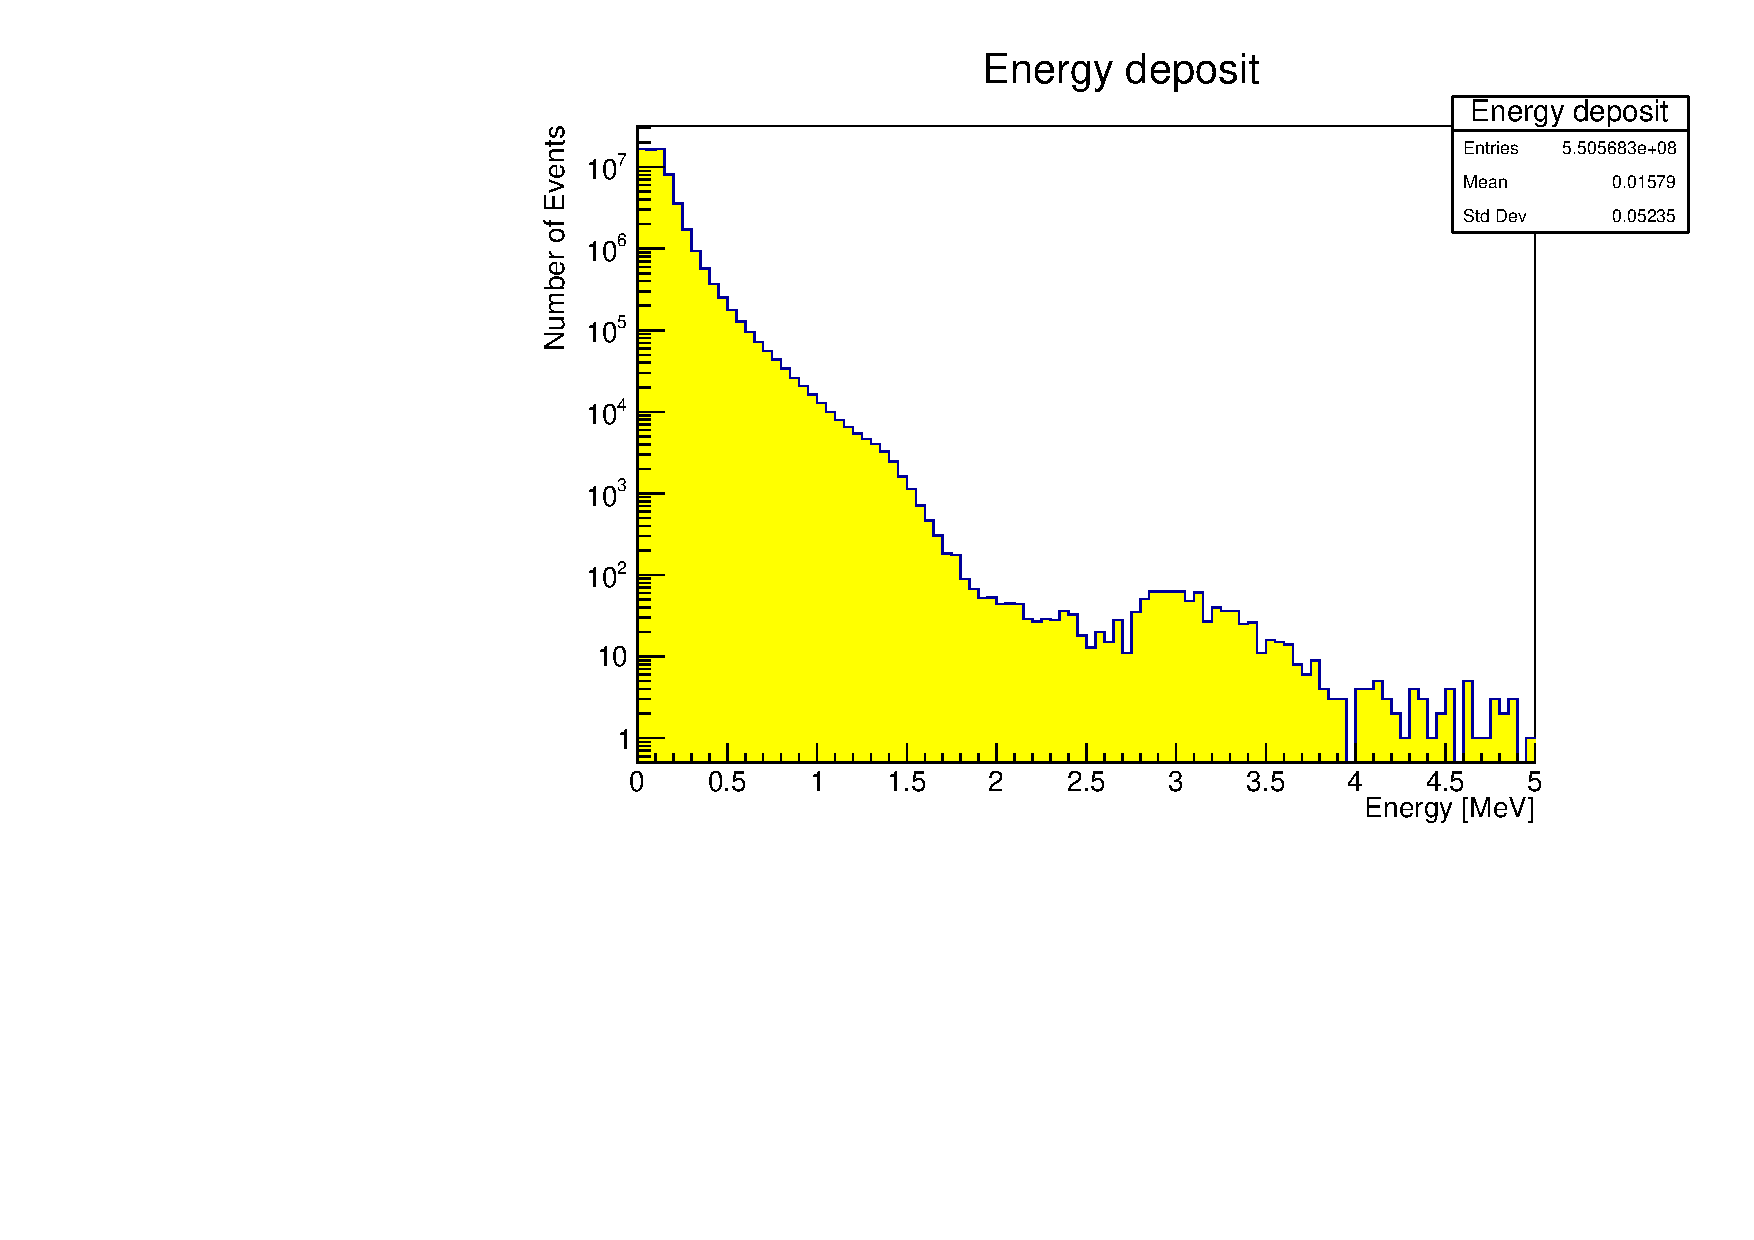
\includegraphics[scale=0.35]{Kap3/pi0_scintillator_electrons_plots_energy_hist.pdf}\label{fig:energy-scintillator-3}}

  \caption{Energy deposit in the scintillator plates of the calorimeter.}\label{fig:energy-scintillator}

\end{figure}

Again, the both cases do not show considerable differences in the particle
distribution along the Z axis, with the only particularity that the electrons
as primary particles have the lowest mean, and the photons the greatest.

It is important to mention that against expected, the average amount of
particles created per event is greater in lead than in the scintillator, the
mean number of photons created in the scintillator is \(261.97\), \(261.119\)
and \(260.267\) when the primary particle is an electron, a photon and a
neutral pion respectively, meanwhile for the lead the averages of photons
generated for the three primary particle are \(10150.9\), \(10119.4\) and
\(10086.8\). It means, in average in the lead the photons are produced almost
four times more than in the scintillator.

The electron production shows similar results, scintillator plates produce in
average \(658.594\), \(655.669\) and \(651.985\) electrons for electrons,
photons and neutral pions as primary particles respectively, but lead plates
produce \(16515\), \(16444\) and \(16346.8\), almost three times more. Note
also that the electron yield is greater than the photon yield for both
materials.

\begin{figure}[htb!]
  \centering

  \subfloat[\(e^-\) as primary particle.]{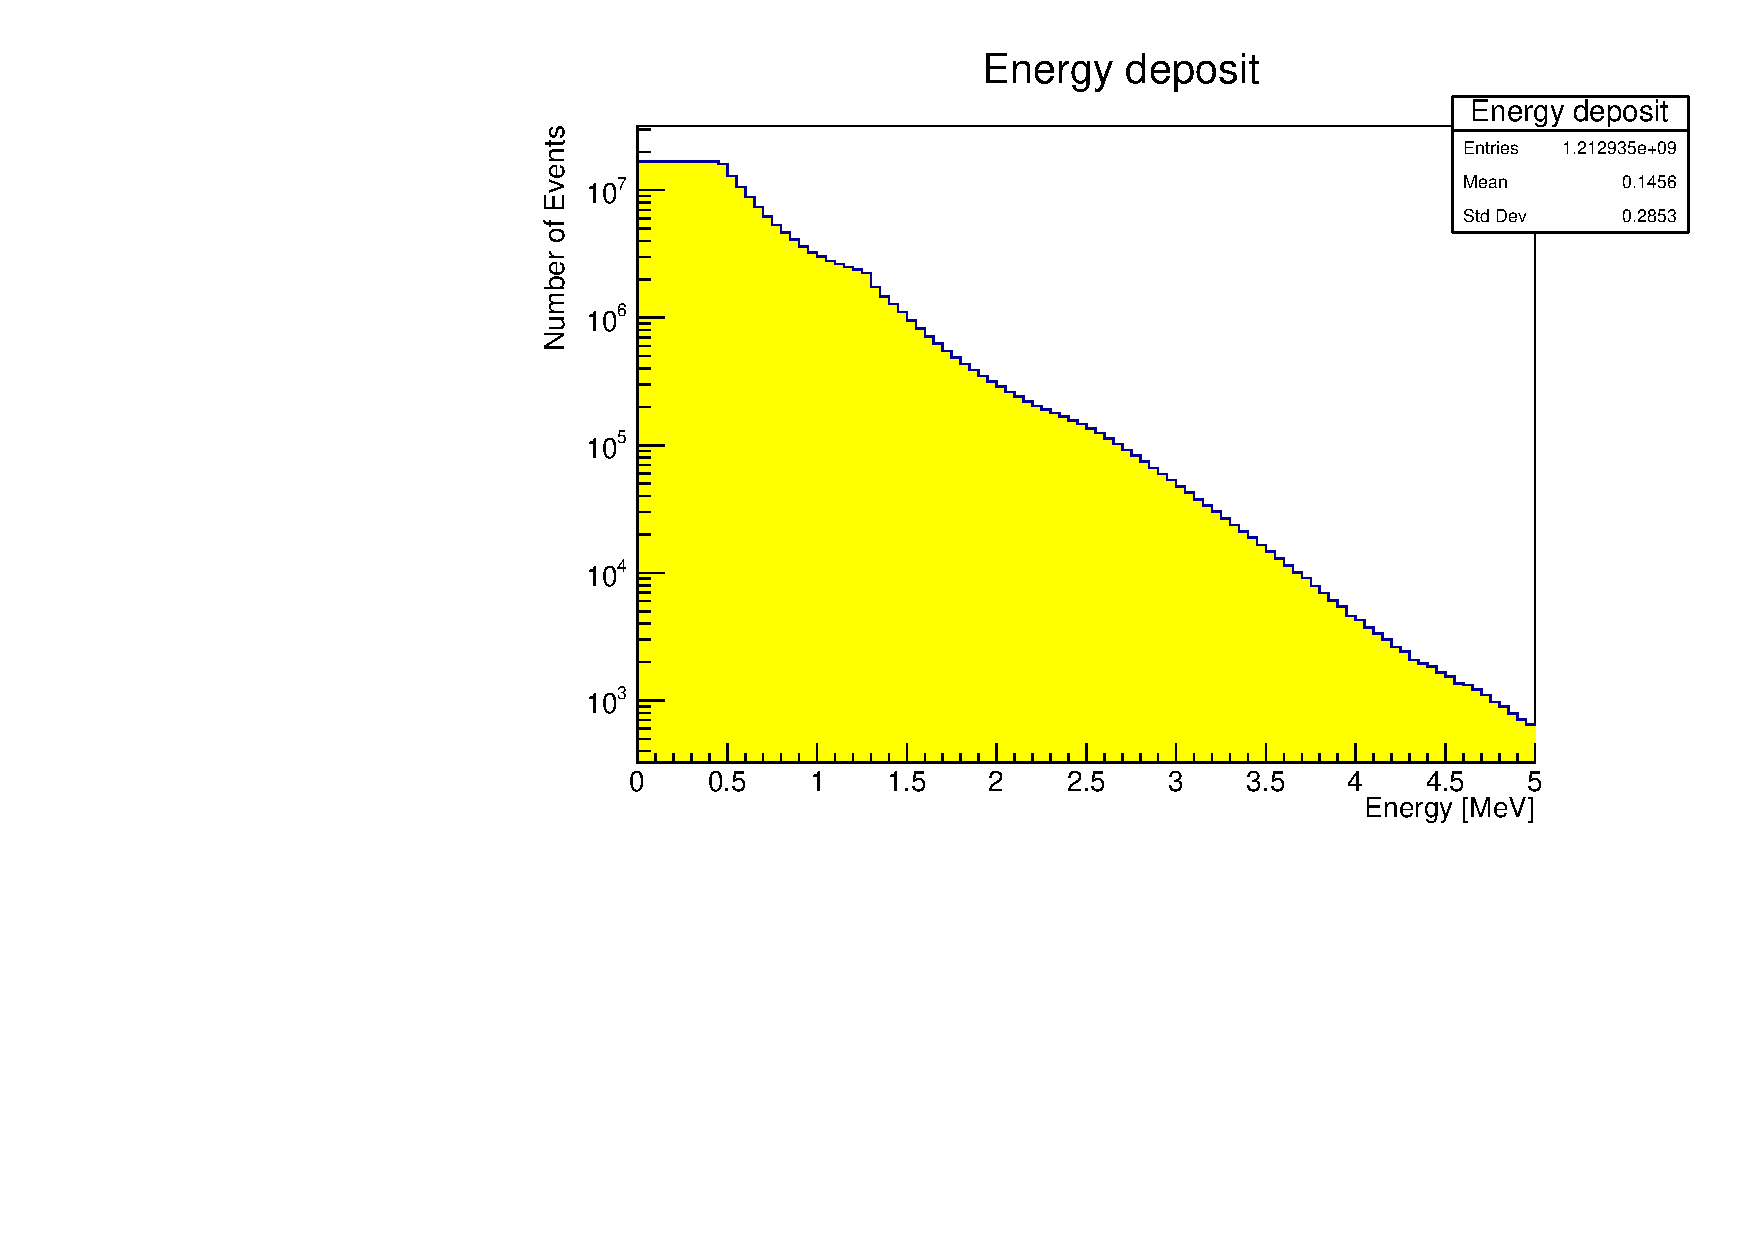
\includegraphics[scale=0.35]{Kap3/electron_lead_electrons_plots_energy_hist.pdf}\label{fig:energy-lead-1}}\hspace{1em}
  \subfloat[\(\gamma\) as primary particle.]{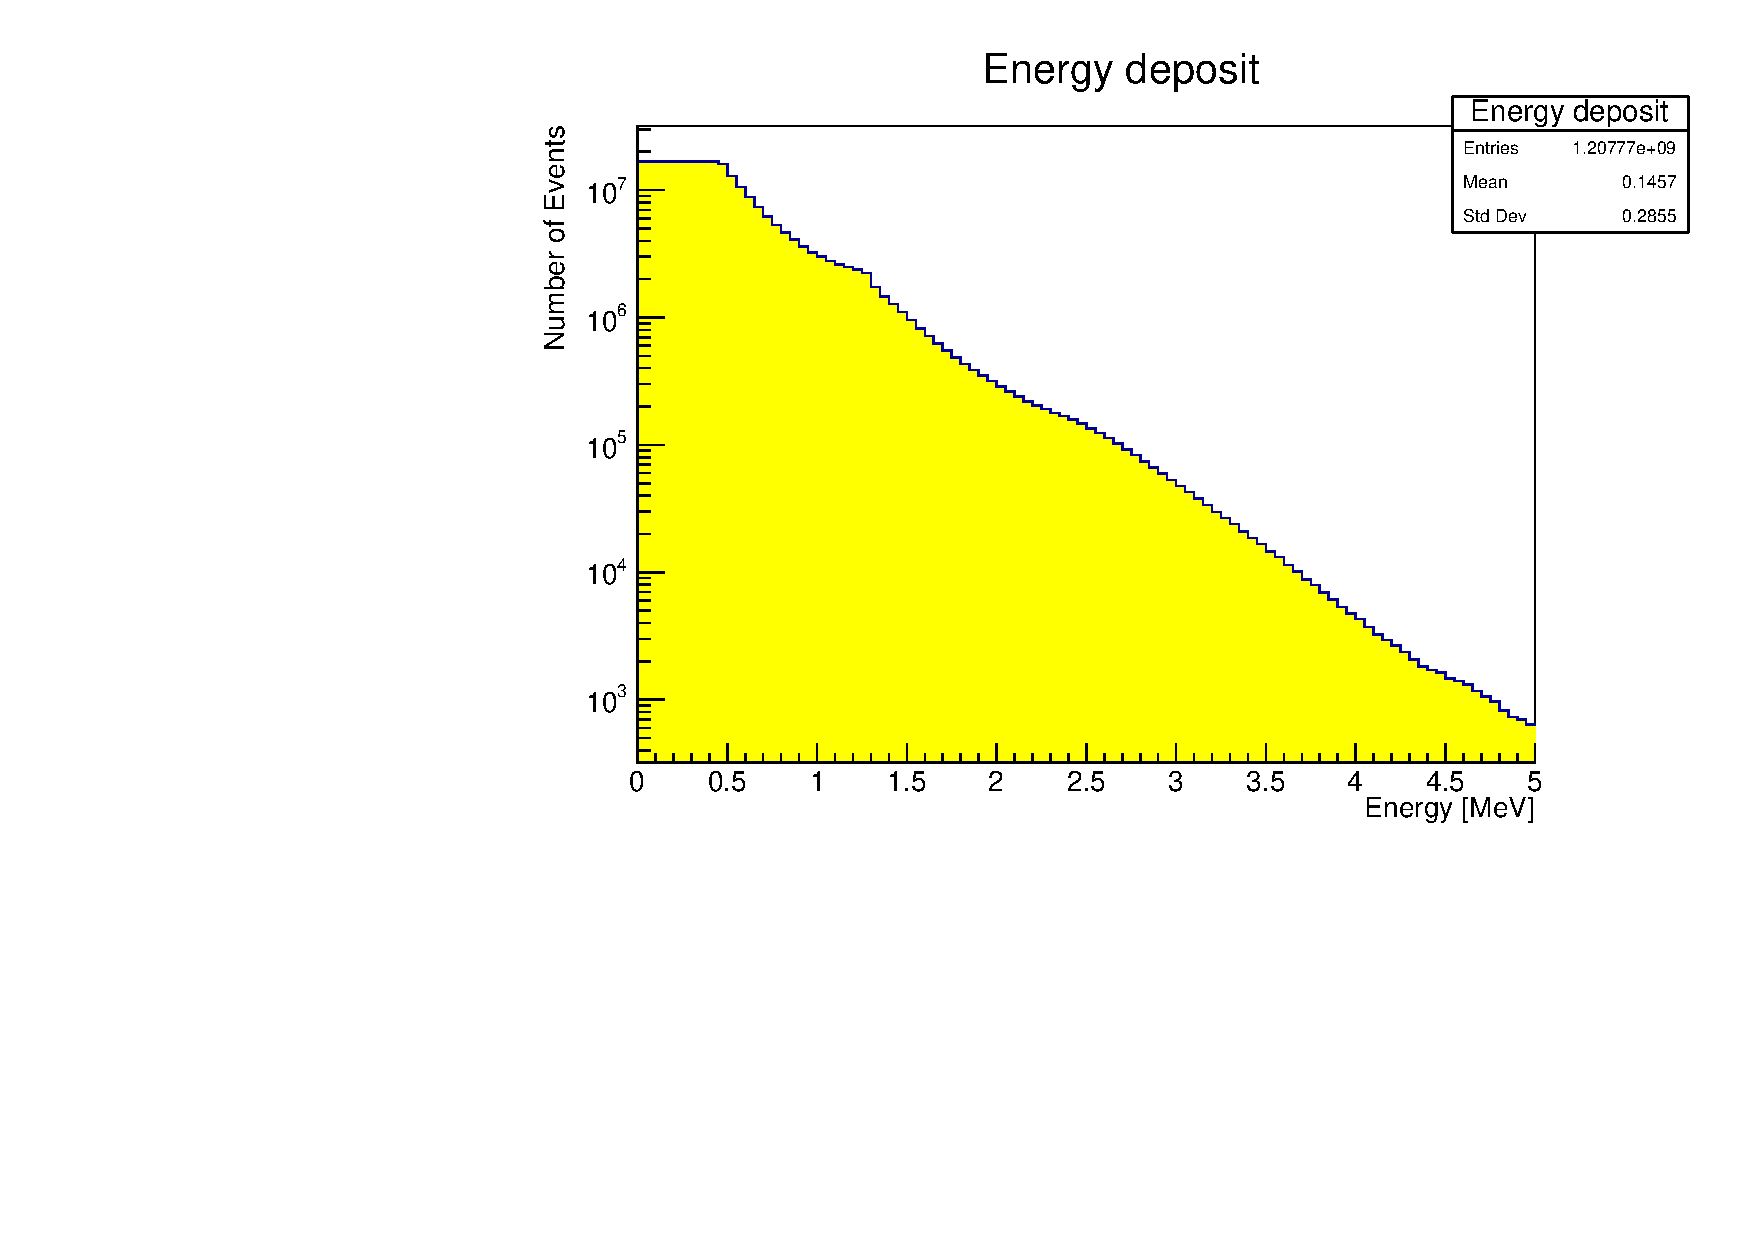
\includegraphics[scale=0.35]{Kap3/gamma_lead_electrons_plots_energy_hist.pdf}\label{fig:energy-lead-2}}\hspace{1em}
  \subfloat[\(\pi^0\) as primary particle.]{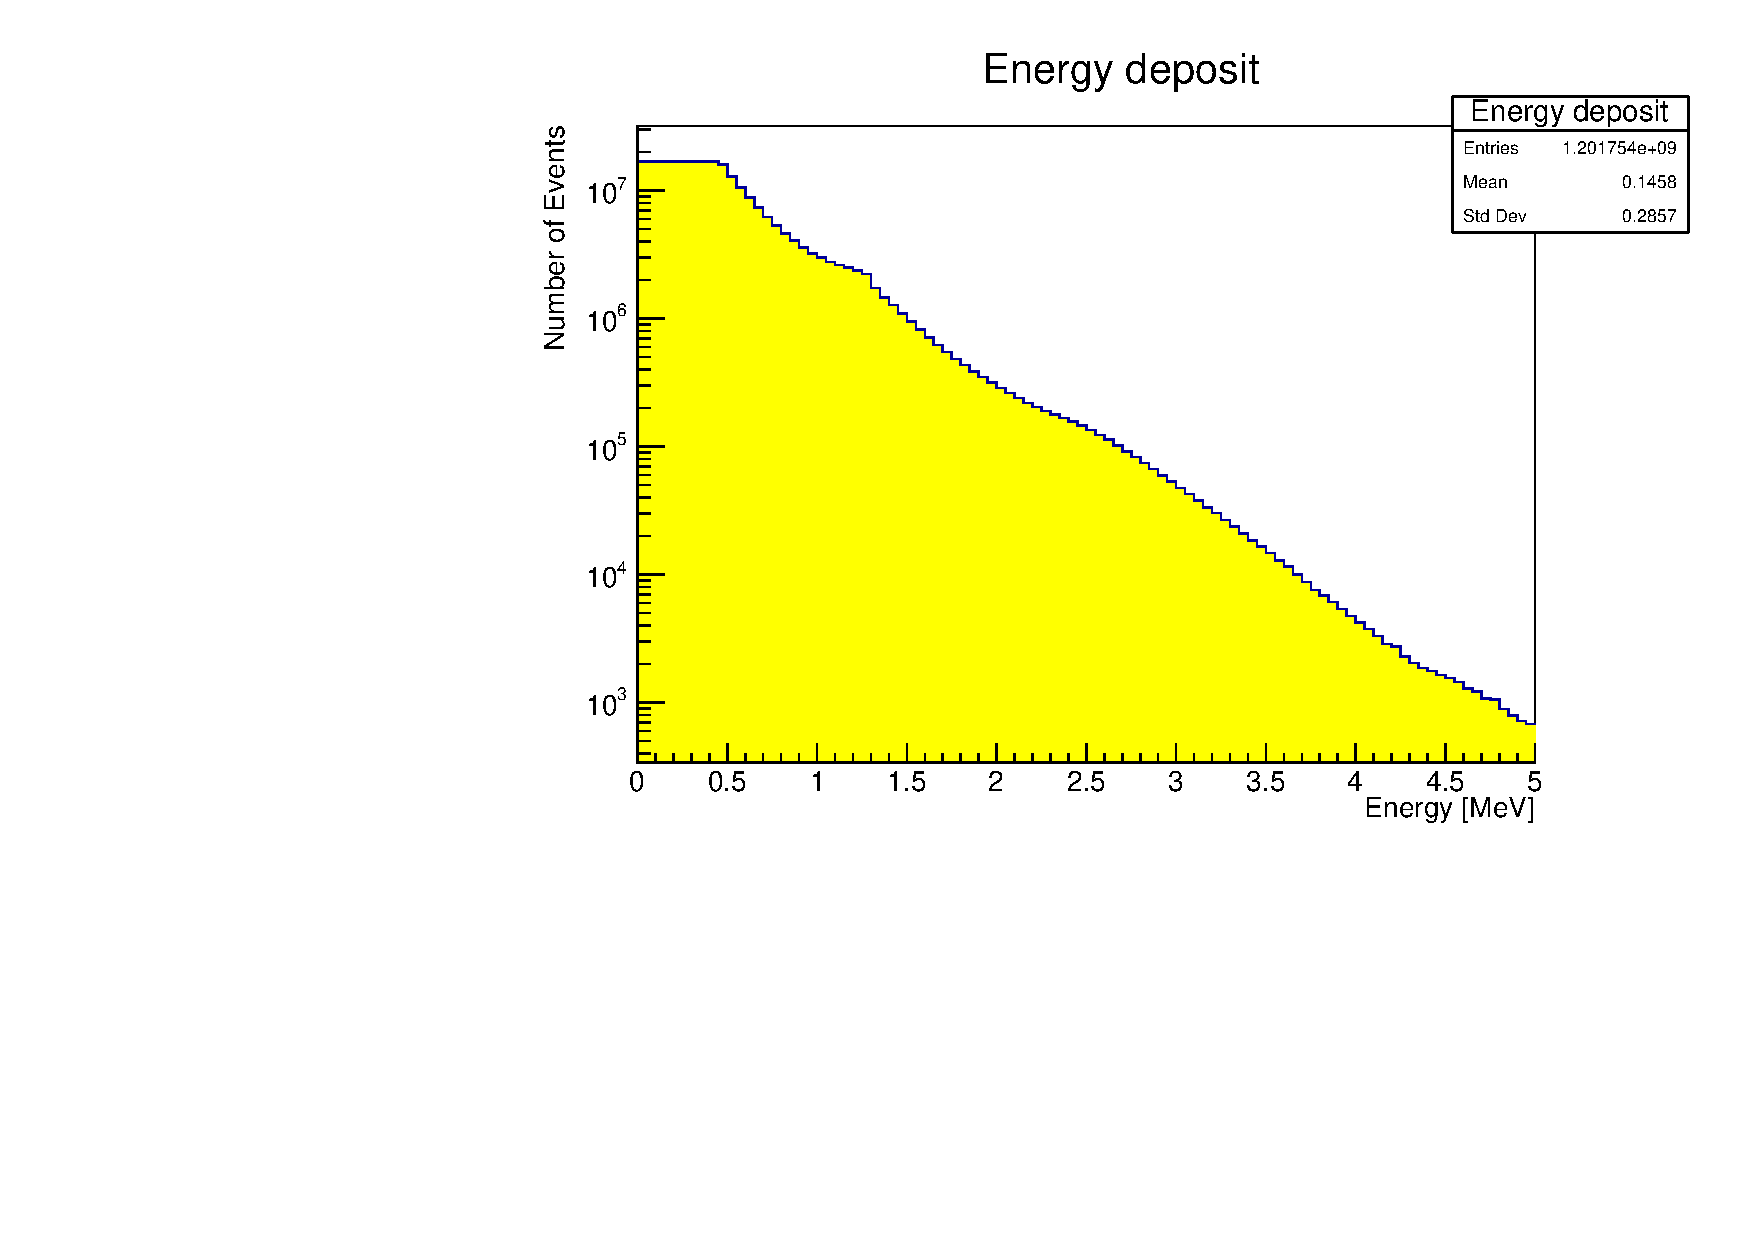
\includegraphics[scale=0.35]{Kap3/pi0_lead_electrons_plots_energy_hist.pdf}\label{fig:energy-lead-3}}

  \caption{Energy deposit in the lead plates of the calorimeter.}\label{fig:energy-lead}

\end{figure}

The energy deposit in the scintillator plates (\cref{fig:energy-scintillator})
and in the lead plates (\cref{fig:energy-lead}) show similar distributions for
all the three primary particles. The same happens to the step length, then, the
results of the Kolmogorov test would determine which cells have significant
different distributions in these two variables to be considered in the machine
learning implementation.

\begin{figure}[htb!]
  \centering

  \subfloat[\(e^-\) as primary particle.]{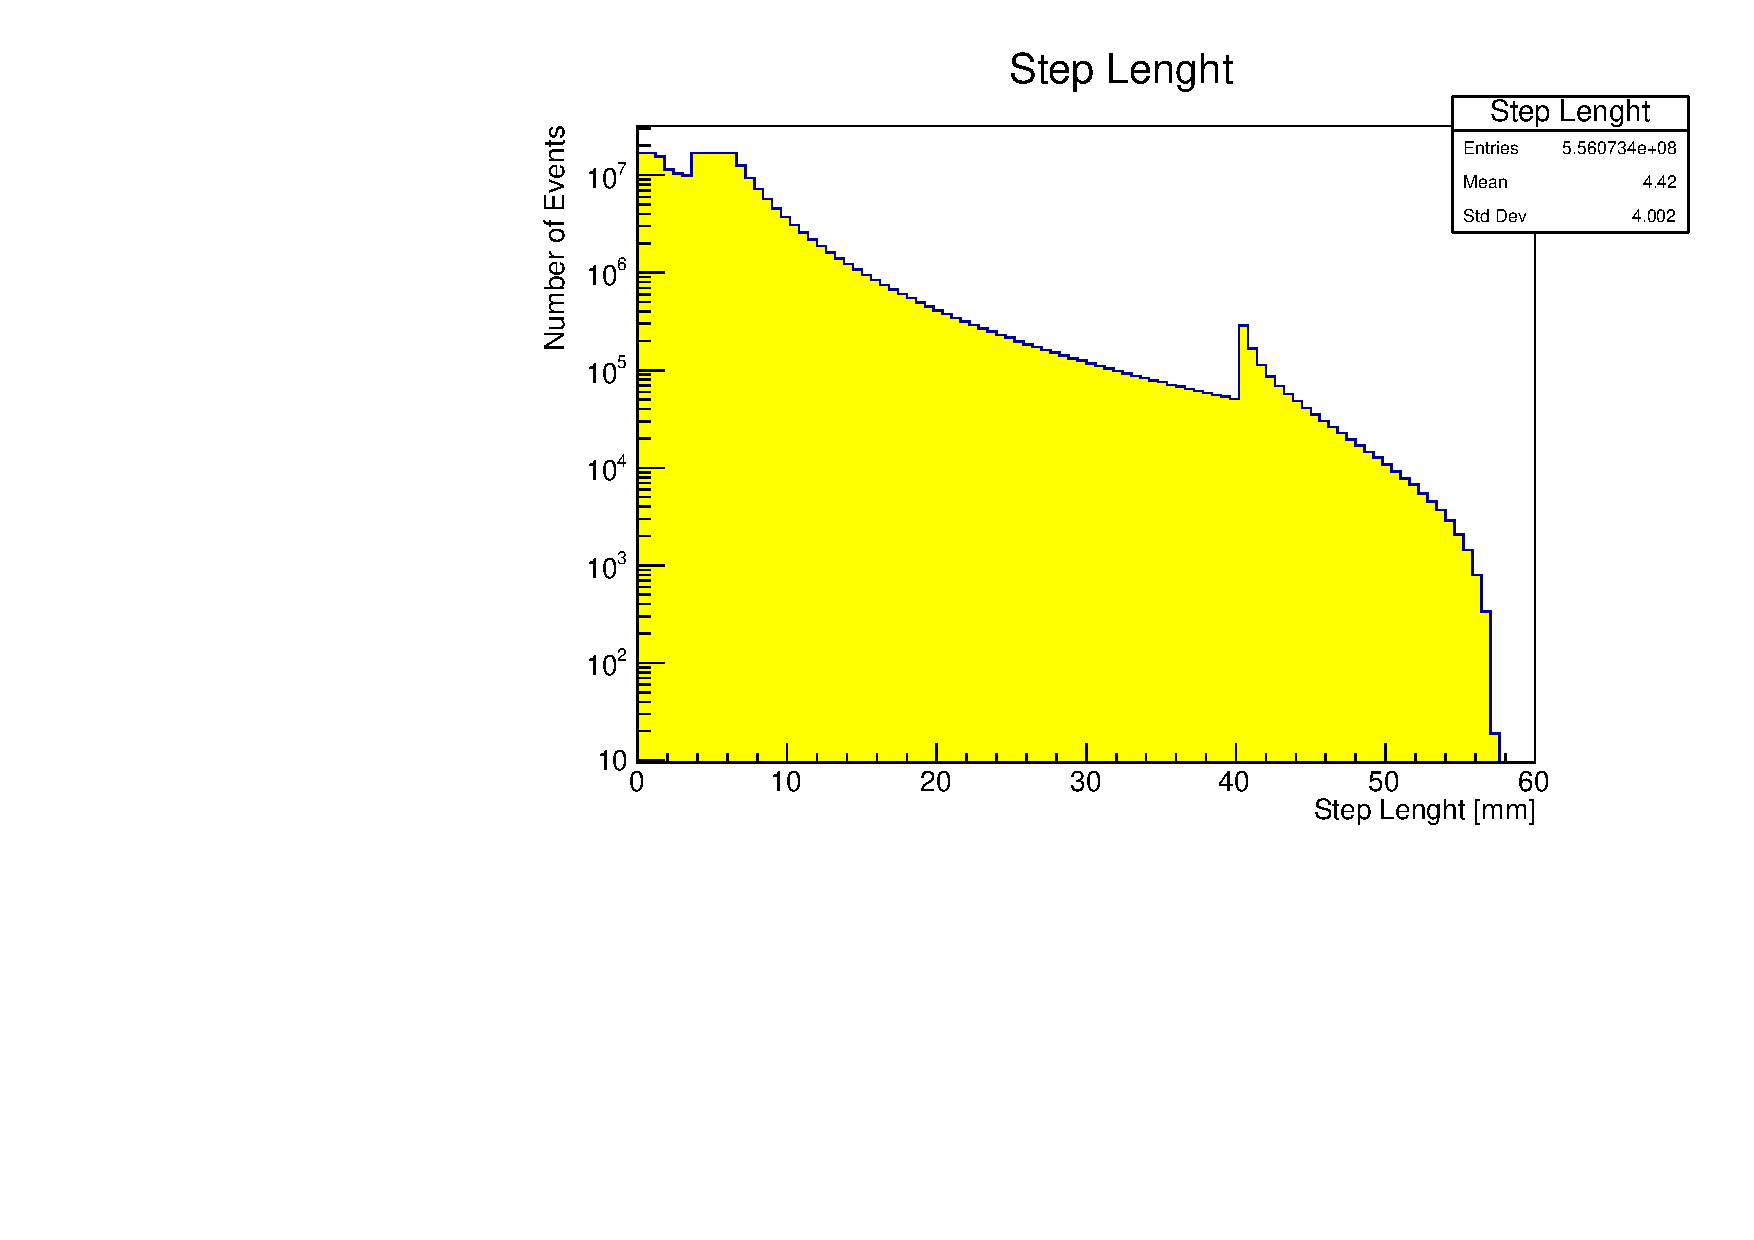
\includegraphics[scale=0.35]{Kap3/electron_scintillator_electrons_plots_step_lengt_hist.pdf}\label{fig:step-lengt-scintillator-1}}\hspace{1em}
  \subfloat[\(\gamma\) as primary particle.]{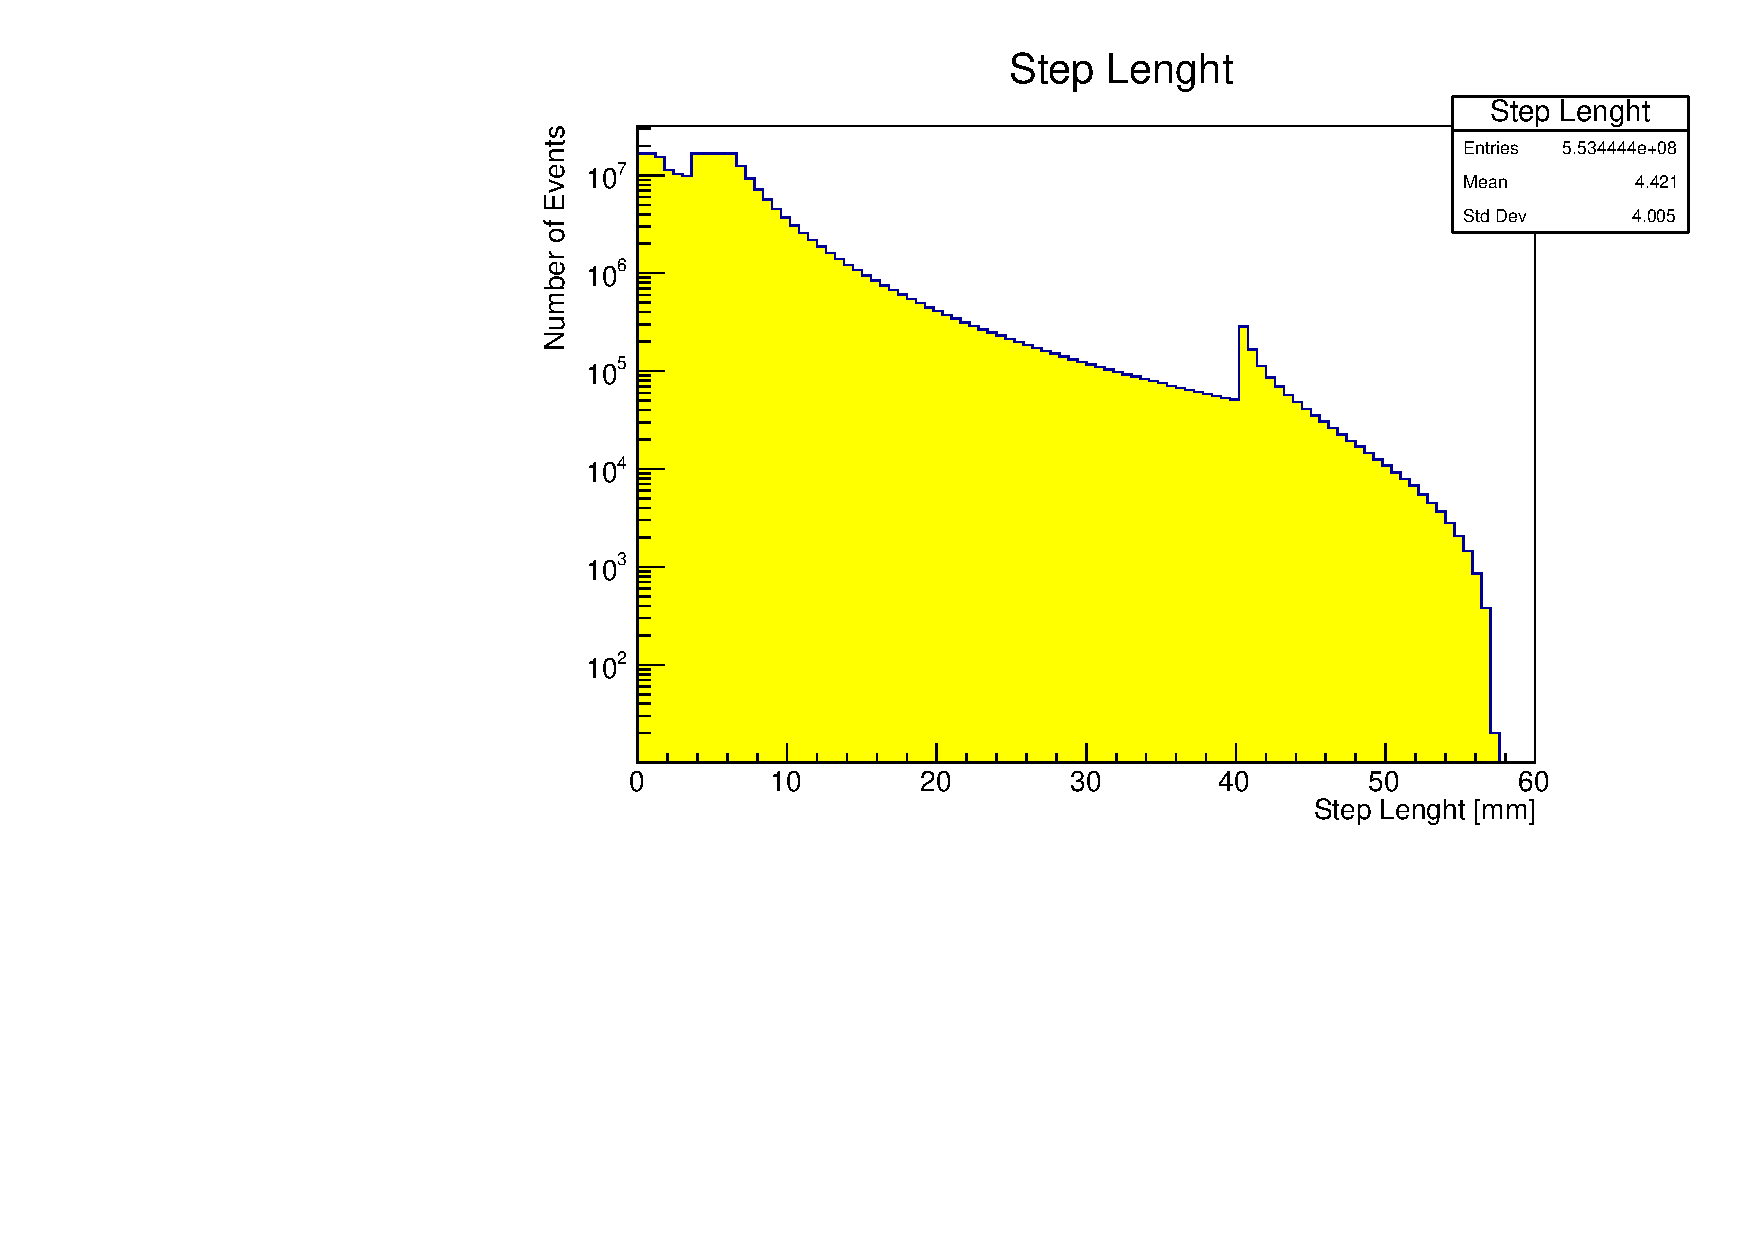
\includegraphics[scale=0.35]{Kap3/gamma_scintillator_electrons_plots_step_lengt_hist.pdf}\label{fig:step-lengt-scintillator-2}}\hspace{1em}
  \subfloat[\(\pi^0\) as primary particle.]{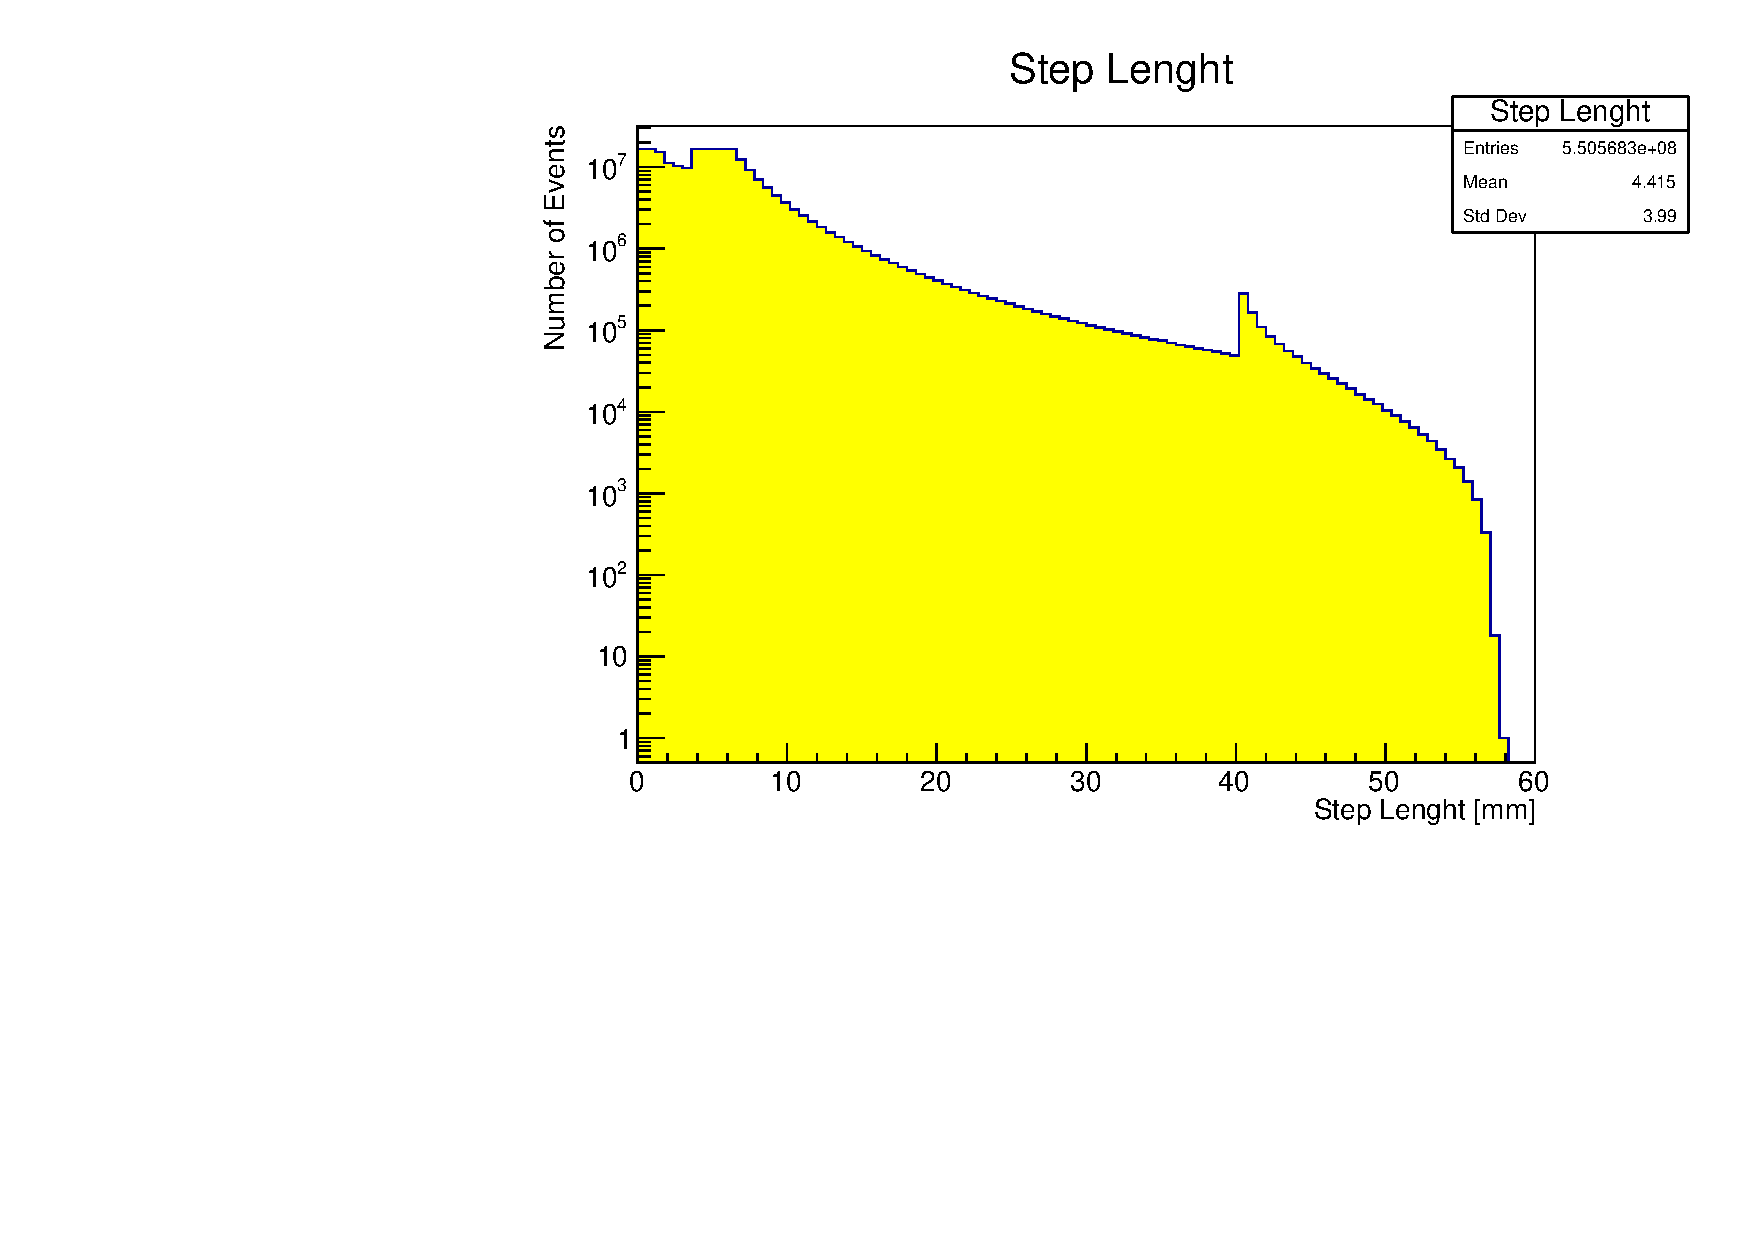
\includegraphics[scale=0.35]{Kap3/pi0_scintillator_electrons_plots_step_lengt_hist.pdf}\label{fig:step-lengt-scintillator-3}}

  \caption{Energy deposit in the scintillator plates of the calorimeter.}\label{fig:step-lengt-scintillator}

\end{figure}

After the Kolmogorov test, from a total of \(16056\) cells, \(14749\) were
tagged as significant for the number of photon created, \(15190\) for the
number of electron created, \(15122\) for the the energy deposit in the plates
and \(15122\) for the step length of the interaction.

\begin{figure}[htb!]
  \centering

  \subfloat[\(e^-\) as primary particle.]{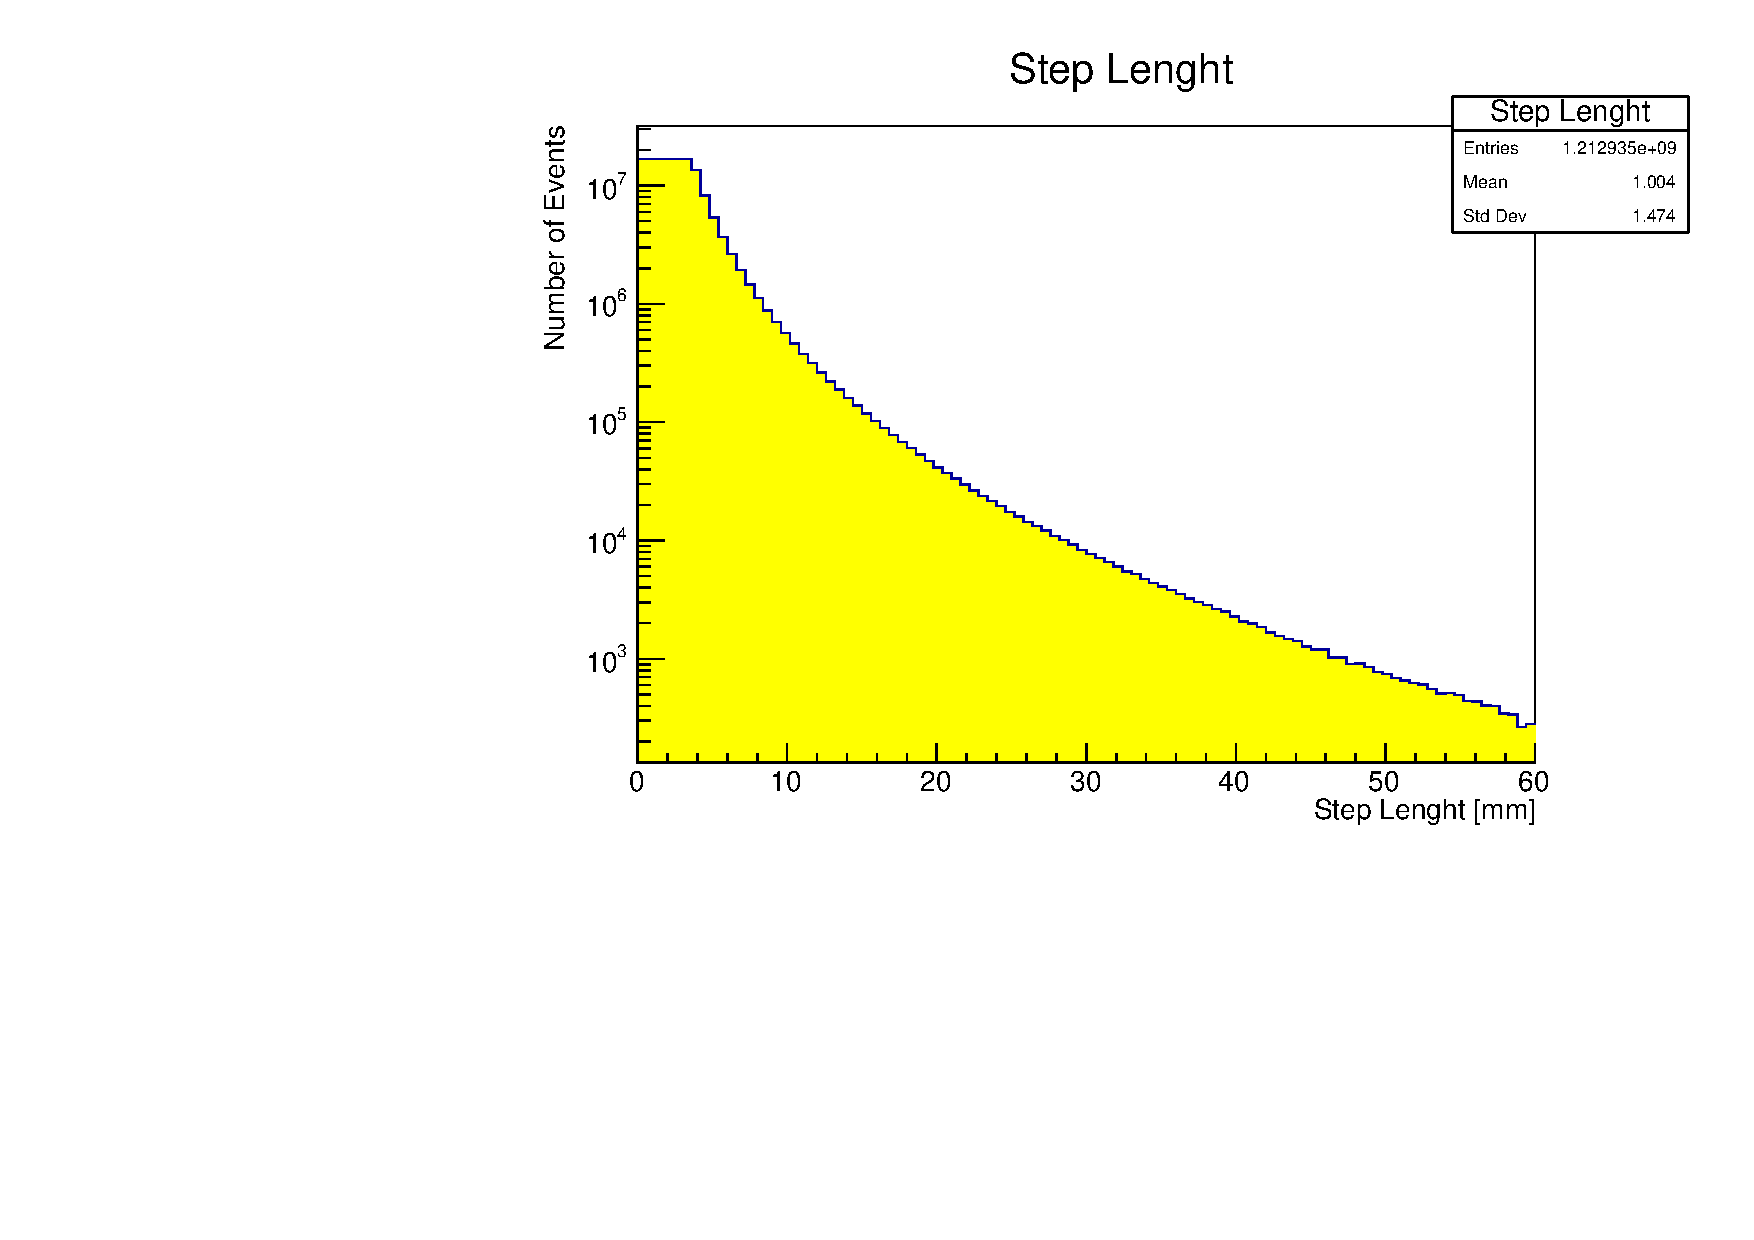
\includegraphics[scale=0.35]{Kap3/electron_lead_electrons_plots_step_lengt_hist.pdf}\label{fig:step-lengt-lead-1}}\hspace{1em}
  \subfloat[\(\gamma\) as primary particle.]{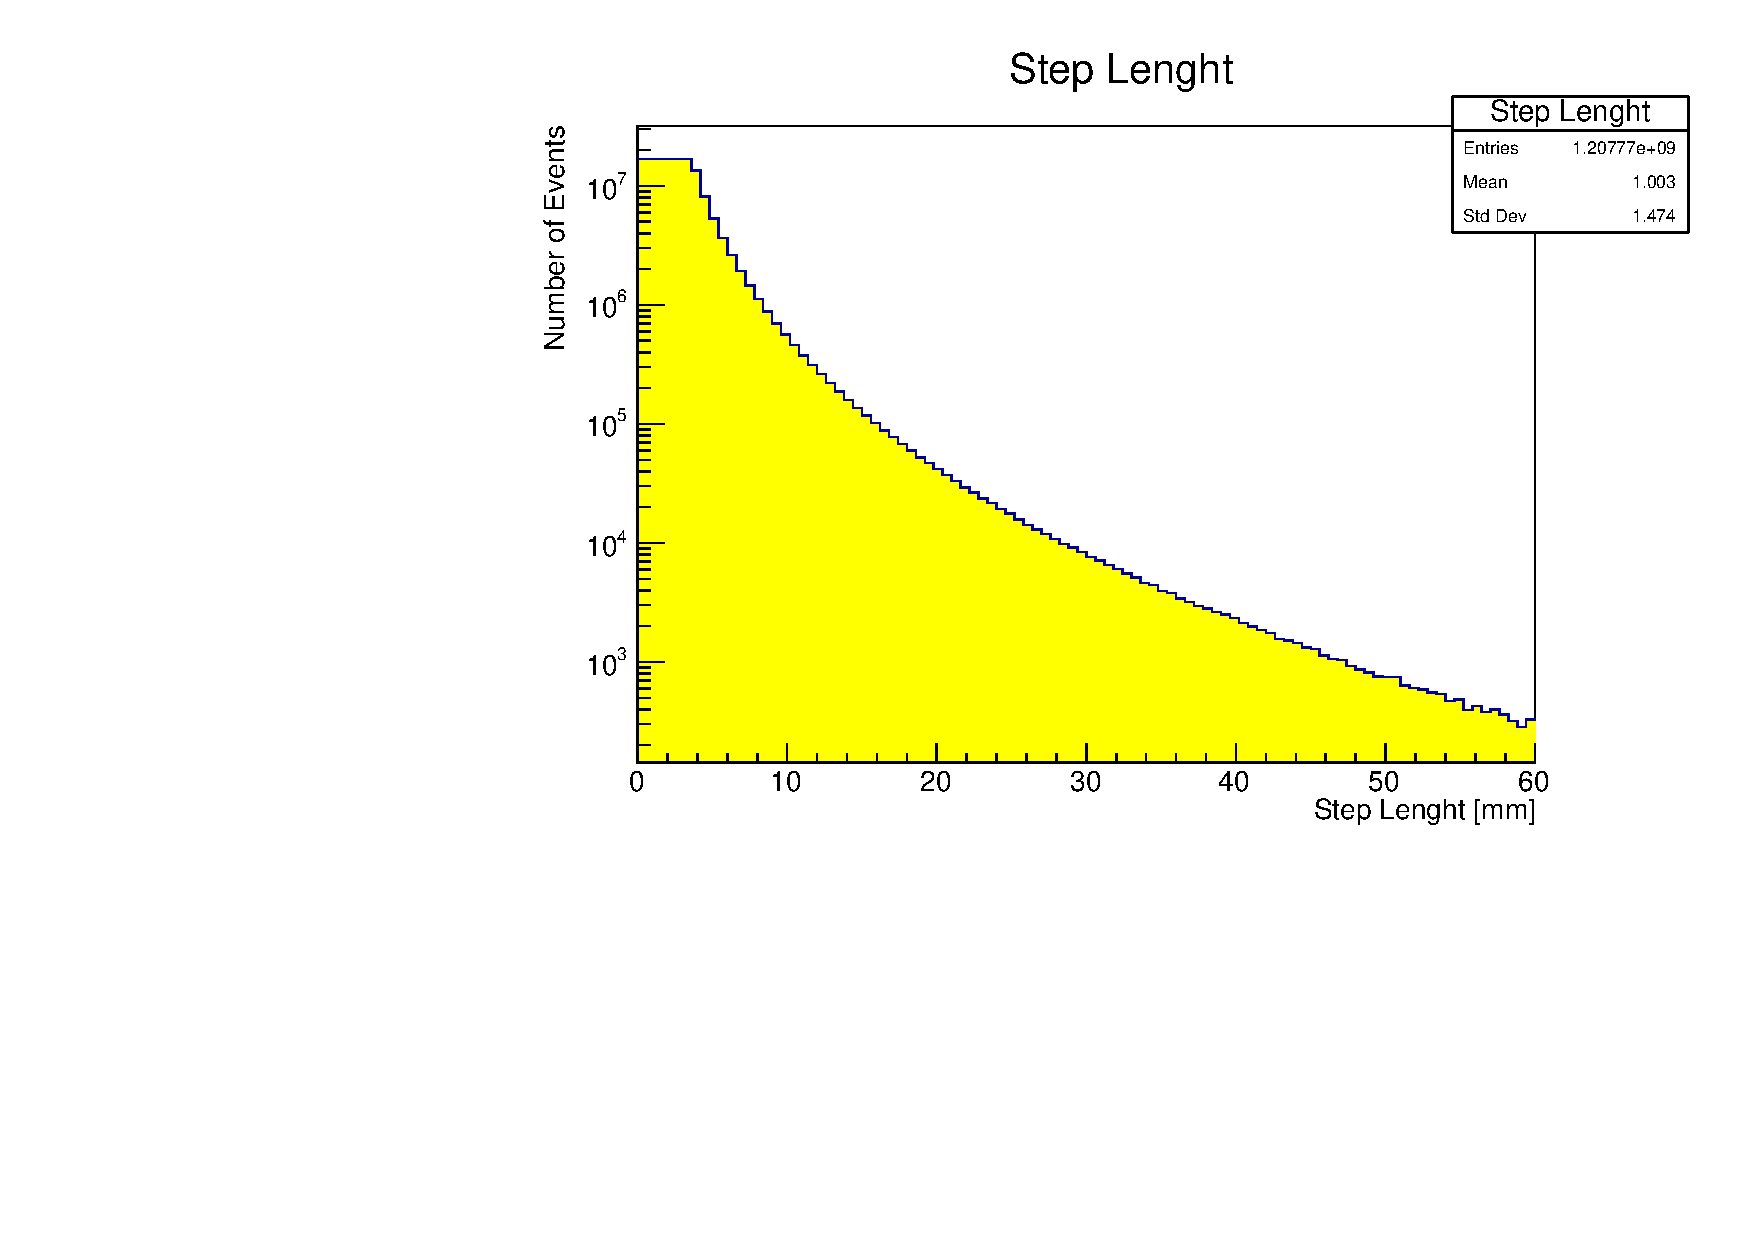
\includegraphics[scale=0.35]{Kap3/gamma_lead_electrons_plots_step_lengt_hist.pdf}\label{fig:step-lengt-lead-2}}\hspace{1em}
  \subfloat[\(\pi^0\) as primary particle.]{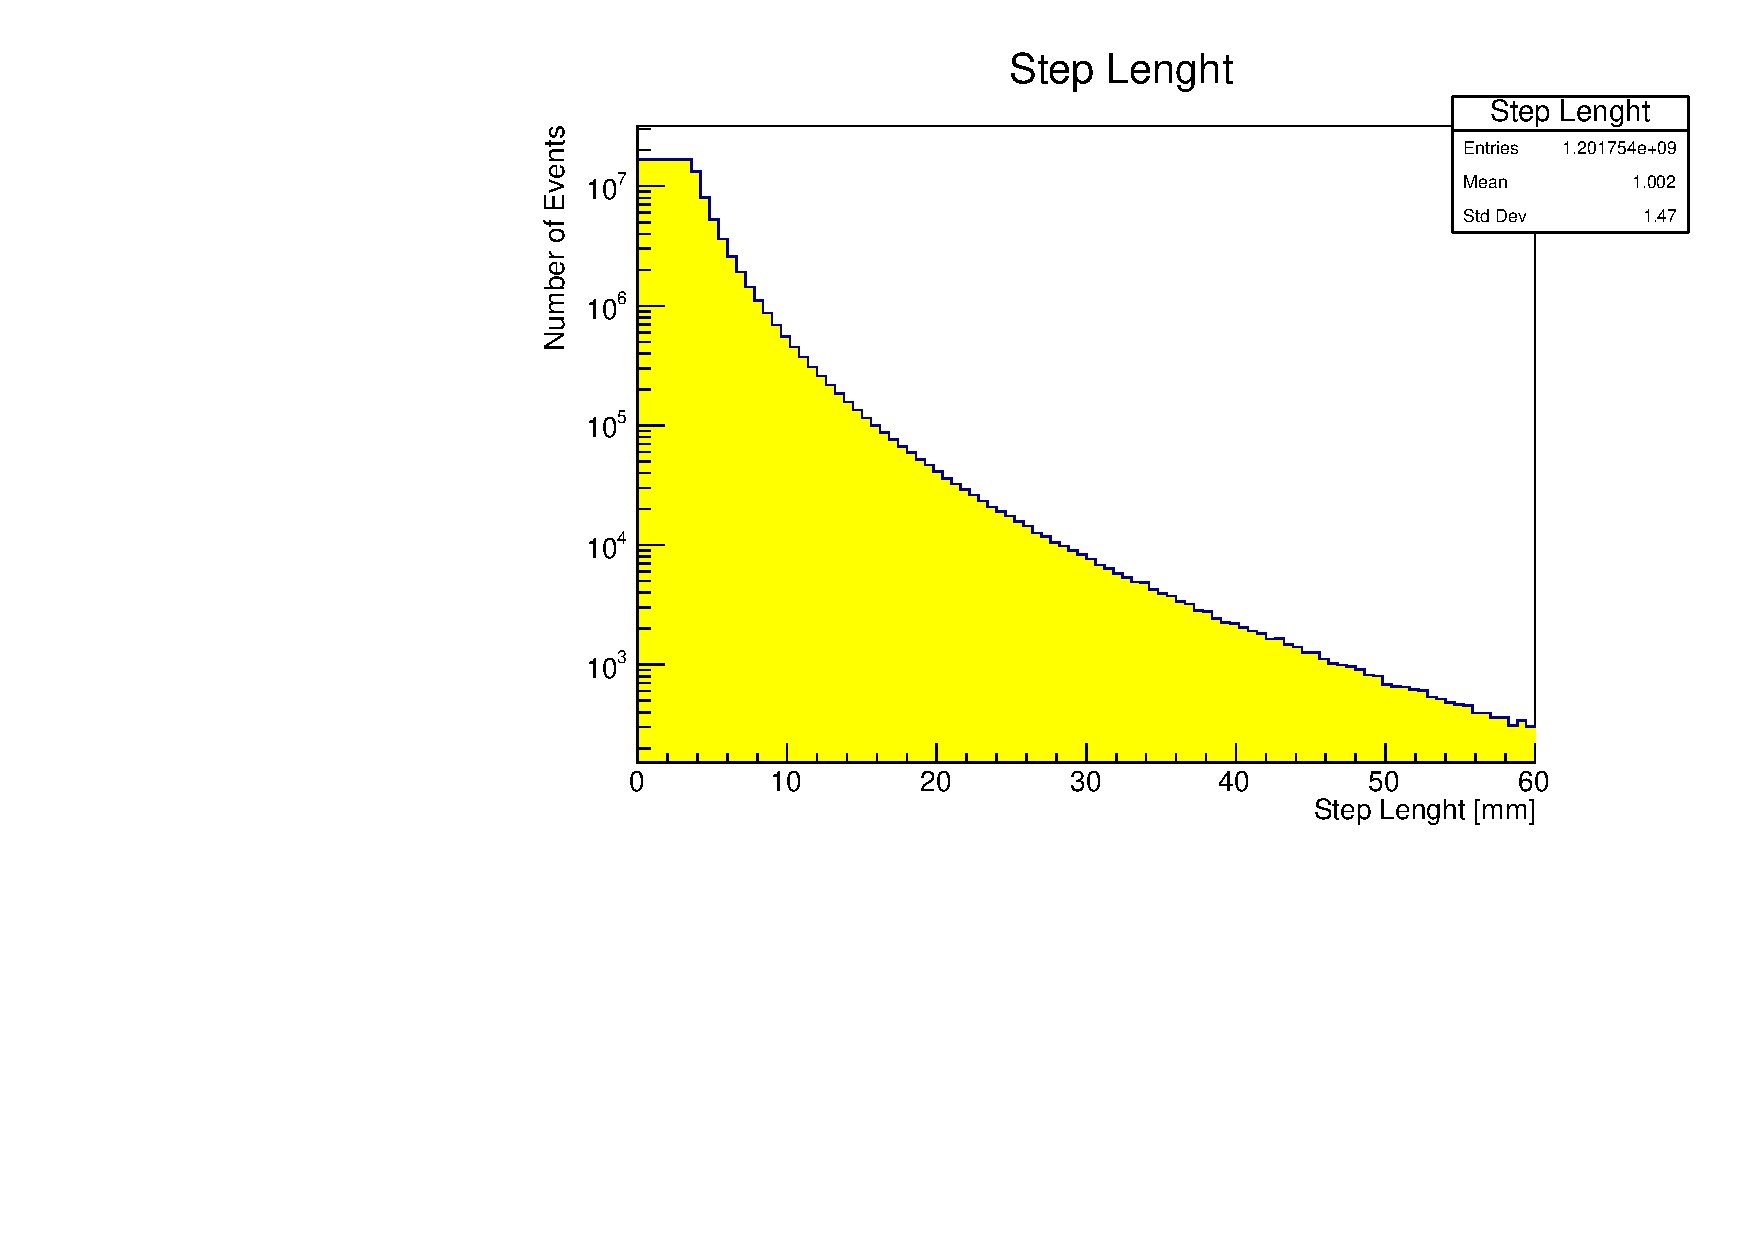
\includegraphics[scale=0.35]{Kap3/pi0_lead_electrons_plots_step_lengt_hist.pdf}\label{fig:step-lengt-lead-3}}

  \caption{Energy deposit in the lead plates of the calorimeter.}\label{fig:step-lengt-lead}

\end{figure}

Finally, the values resulting for the particle creation in the plates, as well
as the energy deposit and step length of the interactions were used as the
input of a machine learning implementation, using the multidimensional
classifiers, MultinomialNB, BernoulliNB, Perceptron, SGDClassifier and
PassiveAggressiveClassifier. The accuracy separating the events according to
the primary particle is shown in the \cref{tb:machine-learning-results}. From
this results, it can be noted that only the BernoulliNB classifier achieved
more than half of the correct answers separating the events, but still did not
get a good accuracy predicting the primary particle.

\begin{table}[hbt]
  \centering
  \begin{tabular}{c c}
    \textbf{Classifier} & \textbf{Result}\\
    \toprule
    MultinomialNB & 0.45\\
    \midrule
    BernoulliNB & 0.55\\
    \midrule
    Perceptron & 0.33\\
    \midrule
    SGDClassifier & 0.33\\
    \midrule
    PassiveAggressiveClassifier & 0.33\\
    \bottomrule
  \end{tabular}
  \caption{Accuracy of the machine learning methods.}\label{tb:machine-learning-results}
\end{table}

For the other methods, it can be seen that they do not predict correctly which
is the incident particle with the given input.

\chapter{Discussion and Conclusions}

The distribution of the particle creation for both scintillator and electrons
in the two materials do not show significant difference between the three
primary particles. The only minor noticeable differences are in the standard
deviation of in the X-Y plane for neutral pion events and in the main value of
the Z-axis distributions, as commented before.

As mentioned above, the number of particles in the scintillator plates per
event is in average lower than in the lead plates, which is unexpected because
scintillator should work as an active material, i.e., produce the major amount
of particles, meanwhile lead is meant to be the absorbent
material\cite{omelaenko2000lhcb}. This issue could be due to unconsidered
material configurations in the Geant4 simulations such as optic settings, that
should increase the number of photons created inside the material.

Some classifiers do not show good performance in the differentiation task,
specially the linear classifiers. It could be due to the amount of variables
that are considered in the input, the low discrepancy between theirs
distributions and the no linearity between them. The best separation was found
for BernoulliNB.

% \chapter{Conclusions}

% \include{Kap6/Kap6}

\addcontentsline{toc}{chapter}{Bibliography}

% \nocite{*}
\printbibliography

\end{document}
